\documentclass[remotesensing,article,submit,pdftex,moreauthors]{Definitions/mdpi} 


\setcounter{secnumdepth}{5}
\setcounter{tocdepth}{5}

%%% ACF I needed subsubsub sections
% Define a fifth level heading that looks like a bold, standalone title
\makeatletter
\providecommand{\subsubsubsection}[1]{%
  \par\bigskip
  \noindent\textbf{#1}\par\nobreak\medskip
}
\makeatother

%\documentclass[preprints,article,submit,pdftex,moreauthors]{Definitions/mdpi} 
% For posting an early version of this manuscript as a preprint, you may use "preprints" as the journal. Changing "submit" to "accept" before posting will remove line numbers.

% Below journals will use APA reference format:
% admsci, aieduc, behavsci, businesses, econometrics, economies, education, ejihpe, famsci, games, humans, ijcs, ijfs, journalmedia, jrfm, languages, psycholint, publications, tourismhosp, youth

% Below journals will use Chicago reference format:
% arts, genealogy, histories, humanities, jintelligence, laws, literature, religions, risks, socsci

%--------------------
% Class Options:
%--------------------
%----------
% journal
%----------
% Choose between the following MDPI journals:
% accountaudit, acoustics, actuators, addictions, adhesives, admsci, adolescents, aerobiology, aerospace, agriculture, agriengineering, agrochemicals, agronomy, ai, air, algorithms, allergies, alloys, amh, analytica, analytics, anatomia, anesthres, animals, antibiotics, antibodies, antioxidants, applbiosci, appliedchem, appliedmath, appliedphys, applmech, applmicrobiol, applnano, applsci, aquacj, architecture, arm, arthropoda, arts, asc, asi, astronomy, atmosphere, atoms, audiolres, automation, axioms, bacteria, batteries, bdcc, behavsci, beverages, biochem, bioengineering, biologics, biology, biomass, biomechanics, biomed, biomedicines, biomedinformatics, biomimetics, biomolecules, biophysica, biosensors, biosphere, biotech, birds, blockchains, bloods, blsf, brainsci, breath, buildings, businesses, cancers, carbon, cardiogenetics, catalysts, cells, ceramics, challenges, chemengineering, chemistry, chemosensors, chemproc, children, chips, cimb, civileng, cleantechnol, climate, clinbioenerg, clinpract, clockssleep, cmd, cmtr, coasts, coatings, colloids, colorants, commodities, complications, compounds, computation, computers, condensedmatter, conservation, constrmater, cosmetics, covid, crops, cryo, cryptography, crystals, csmf, ctn, curroncol, cyber, dairy, data, ddc, dentistry, dermato, dermatopathology, designs, devices, diabetology, diagnostics, dietetics, digital, disabilities, diseases, diversity, dna, drones, dynamics, earth, ebj, ecm, ecologies, econometrics, economies, education, eesp, ejihpe, electricity, electrochem, electronicmat, electronics, encyclopedia, endocrines, energies, eng, engproc, ent, entomology, entropy, environments, epidemiologia, epigenomes, esa, est, famsci, fermentation, fibers, fintech, fire, fishes, fluids, foods, forecasting, forensicsci, forests, fossstud, foundations, fractalfract, fuels, future, futureinternet, futureparasites, futurepharmacol, futurephys, futuretransp, galaxies, games, gases, gastroent, gastrointestdisord, gastronomy, gels, genealogy, genes, geographies, geohazards, geomatics, geometry, geosciences, geotechnics, geriatrics, glacies, grasses, greenhealth, gucdd, hardware, hazardousmatters, healthcare, hearts, hemato, hematolrep, heritage, higheredu, highthroughput, histories, horticulturae, hospitals, humanities, humans, hydrobiology, hydrogen, hydrology, hygiene, idr, iic, ijerph, ijfs, ijgi, ijmd, ijms, ijns, ijpb, ijt, ijtm, ijtpp, ime, immuno, informatics, information, infrastructures, inorganics, insects, instruments, inventions, iot, j, jal, jcdd, jcm, jcp, jcs, jcto, jdad, jdb, jeta, jfb, jfmk, jimaging, jintelligence, jlpea, jmahp, jmmp, jmms, jmp, jmse, jne, jnt, jof, joitmc, joma, jop, jor, journalmedia, jox, jpbi, jpm, jrfm, jsan, jtaer, jvd, jzbg, kidney, kidneydial, kinasesphosphatases, knowledge, labmed, laboratories, land, languages, laws, life, lights, limnolrev, lipidology, liquids, literature, livers, logics, logistics, lubricants, lymphatics, machines, macromol, magnetism, magnetochemistry, make, marinedrugs, materials, materproc, mathematics, mca, measurements, medicina, medicines, medsci, membranes, merits, metabolites, metals, meteorology, methane, metrics, metrology, micro, microarrays, microbiolres, microelectronics, micromachines, microorganisms, microplastics, microwave, minerals, mining, mmphys, modelling, molbank, molecules, mps, msf, mti, multimedia, muscles, nanoenergyadv, nanomanufacturing, nanomaterials, ncrna, ndt, network, neuroglia, neurolint, neurosci, nitrogen, notspecified, nursrep, nutraceuticals, nutrients, obesities, oceans, ohbm, onco, oncopathology, optics, oral, organics, organoids, osteology, oxygen, parasites, parasitologia, particles, pathogens, pathophysiology, pediatrrep, pets, pharmaceuticals, pharmaceutics, pharmacoepidemiology, pharmacy, philosophies, photochem, photonics, phycology, physchem, physics, physiologia, plants, plasma, platforms, pollutants, polymers, polysaccharides, populations, poultry, powders, preprints, proceedings, processes, prosthesis, proteomes, psf, psych, psychiatryint, psychoactives, psycholint, publications, purification, quantumrep, quaternary, qubs, radiation, reactions, realestate, receptors, recycling, regeneration, religions, remotesensing, reports, reprodmed, resources, rheumato, risks, robotics, rsee, ruminants, safety, sci, scipharm, sclerosis, seeds, sensors, separations, sexes, signals, sinusitis, siuj, skins, smartcities, sna, societies, socsci, software, soilsystems, solar, solids, spectroscj, sports, standards, stats, std, stresses, surfaces, surgeries, suschem, sustainability, symmetry, synbio, systems, tae, targets, taxonomy, technologies, telecom, test, textiles, thalassrep, therapeutics, thermo, timespace, tomography, tourismhosp, toxics, toxins, transplantology, transportation, traumacare, traumas, tropicalmed, universe, urbansci, uro, vaccines, vehicles, venereology, vetsci, vibration, virtualworlds, viruses, vision, waste, water, wem, wevj, wild, wind, women, world, youth, zoonoticdis

%---------
% article
%---------
% The default type of manuscript is "article", but can be replaced by: 
% abstract, addendum, article, benchmark, book, bookreview, briefcommunication, briefreport, casereport, changes, clinicopathologicalchallenge, comment, commentary, communication, conceptpaper, conferenceproceedings, correction, conferencereport, creative, datadescriptor, discussion, entry, expressionofconcern, extendedabstract, editorial, essay, erratum, fieldguide, hypothesis, interestingimages, letter, meetingreport, monograph, newbookreceived, obituary, opinion, proceedingpaper, projectreport, reply, retraction, review, perspective, protocol, shortnote, studyprotocol, supfile, systematicreview, technicalnote, viewpoint, guidelines, registeredreport, tutorial,  giantsinurology, urologyaroundtheworld
% supfile = supplementary materials

%----------
% submit
%----------
% The class option "submit" will be changed to "accept" by the Editorial Office when the paper is accepted. This will only make changes to the frontpage (e.g., the logo of the journal will get visible), the headings, and the copyright information. Also, line numbering will be removed. Journal info and pagination for accepted papers will also be assigned by the Editorial Office.

%------------------
% moreauthors
%------------------
% If there is only one author the class option oneauthor should be used. Otherwise use the class option moreauthors.

%---------
% pdftex
%---------
% The option pdftex is for use with pdfLaTeX. Remove "pdftex" for (1) compiling with LaTeX & dvi2pdf (if eps figures are used) or for (2) compiling with XeLaTeX.

%=================================================================
% MDPI internal commands - do not modify
\firstpage{1} 
\makeatletter 
\setcounter{page}{\@firstpage} 
\makeatother
\pubvolume{1}
\issuenum{1}
\articlenumber{0}
\pubyear{2025}
\copyrightyear{2025}
%\externaleditor{Firstname Lastname} % More than 1 editor, please add `` and '' before the last editor name
\datereceived{ } 
\daterevised{ } % Comment out if no revised date
\dateaccepted{ } 
\datepublished{ } 
%\datecorrected{} % For corrected papers: "Corrected: XXX" date in the original paper.
%\dateretracted{} % For retracted papers: "Retracted: XXX" date in the original paper.
\hreflink{https://doi.org/} % If needed use \linebreak
%\doinum{}
%\pdfoutput=1 % Uncommented for upload to arXiv.org
%\CorrStatement{yes}  % For updates
%\longauthorlist{yes} % For many authors that exceed the left citation part

%=================================================================
% Add packages and commands here. The following packages are loaded in our class file: fontenc, inputenc, calc, indentfirst, fancyhdr, graphicx, epstopdf, lastpage, ifthen, float, amsmath, amssymb, lineno, setspace, enumitem, mathpazo, booktabs, titlesec, etoolbox, tabto, xcolor, colortbl, soul, multirow, microtype, tikz, totcount, changepage, attrib, upgreek, array, tabularx, pbox, ragged2e, tocloft, marginnote, marginfix, enotez, amsthm, natbib, hyperref, cleveref, scrextend, url, geometry, newfloat, caption, draftwatermark, seqsplit
% cleveref: load \crefname definitions after \begin{document}

%=================================================================
% Please use the following mathematics environments: Theorem, Lemma, Corollary, Proposition, Characterization, Property, Problem, Example, ExamplesandDefinitions, Hypothesis, Remark, Definition, Notation, Assumption
%% For proofs, please use the proof environment (the amsthm package is loaded by the MDPI class).

%=================================================================
% Full title of the paper (Capitalized)
%%% AAB - Repensar o título, pois usamos também nos resultados pdf físicas.
\Title{Fast Spatial Denoising for Repeat-Pass InSAR Data via Empirical Statistical Modeling}

% MDPI internal command: Title for citation in the left column
\TitleCitation{Fast Spatial Denoising for Repeat-Pass InSAR Data via Empirical Statistical Modeling}

% Author Orchid ID: enter ID or remove command
%\newcommand{\orcidauthorA}{0000-0002-7849-9572} % Add \orcidA{} behind the author's name
%\newcommand{\orcidauthorB}{0000-0000-0000-000X} % Add \orcidB{} behind the author's name


\Author{Anderson A.\ De Borba$^{1,*}$\href{https://orcid.org/0000-0001-8479-9128}
	{\orcidicon},
	Joselito E.\ De Araújo$^{2}$\href{https://orcid.org/0000-0002-7849-9572}
	{\orcidicon},  
	Alejandro C. Frery$^{3}$\href{https://orcid.org/0000-0002-8002-5341}
	{\orcidicon}}


%\longauthorlist{yes}

% MDPI internal command: Authors, for metadata in PDF
\AuthorNames{Anderson A.\ de Borba, Joselito E.\ de Araújo, and Alejandro C.\ Frery}

% MDPI internal command: Authors, for citation in the left column, only choose below one of them according to the journal style
% If this is a Chicago style journal 
% (arts, genealogy, histories, humanities, jintelligence, laws, literature, religions, risks, socsci): 
% Lastname, Firstname, Firstname Lastname, and Firstname Lastname.

% If this is a APA style journal 
% (admsci, behavsci, businesses, econometrics, economies, education, ejihpe, games, humans, ijfs, journalmedia, jrfm, languages, psycholint, publications, tourismhosp, youth): 
% Lastname, F., Lastname, F., \& Lastname, F.

% If this is a ACS style journal (Except for the above Chicago and APA journals, all others are in the ACS format): 
% Lastname, F.; Lastname, F.; Lastname, F.
\isAPAStyle{%
	\AuthorCitation{Borba, A. A., Araújo, J. E., \& Frery, A. C.}%
}{%
	\isChicagoStyle{%
		\AuthorCitation{Anderson A. de Borba, Araújo, Joselito Elias, and Alejandro C. Frery.}%
	}{%
		\AuthorCitation{Borba, A. A.; Araújo, J. E.; Frery, A. C.}%
	}%
}

% Affiliations / Addresses (Add [1] after \address if there is only one affiliation.)
\address{%
	$^{1}$\quad Computing and Informatics Department - FCI - DataLab, Mackenzie Presbyterian University (MPU); anderson.borba@mackenzie.br\\
	$^{2}$\quad Department of Statistics, Federal University of Pernambuco, Recife 50670-901, PE, Brazil; joselito.araujo@ufpe.br\\
	$^{3}$\quad School of Mathematics and Statistics, Victoria University
	of Wellington, 6140 New Zealand; alejandro.frery@vuw.ac.nz
}

% Contact information of the corresponding author
\corres{Correspondence: anderson.borba@mackenzie.br; Tel.: +55~11~98456-3218.}

% Current address and/or shared authorship
%\firstnote{Current address: Affiliation.}  
% Current address should not be the same as any items in the Affiliation section.

%\secondnote{These authors contributed equally to this work.}
% The commands \thirdnote{} till \eighthnote{} are available for further notes.

%\simplesumm{} % Simple summary

%\conference{} % An extended version of a conference paper

% Abstract (Do not insert blank lines, i.e. \\) 
\abstract{
Repeat-pass SAR interferometry (InSAR) provides a framework for extracting high-resolution topographic information and detecting surface deformation. 
By analyzing the phase difference between radar acquisitions obtained at different times, one can characterize landscape geometry and surface changes. 
However, inherent phase noise often compromises the reliability of the resulting interferometric products. 
Consequently, there is a sustained need for spatial filtering techniques that suppress noise while preserving structural integrity and resolution.
%
This work evaluates three statistically-based spatial filters. 
We examine a model derived from the physical properties of coherent illumination (the Gierull model) and compare it against two empirical alternatives: the truncated wrapped normal (TcN) and the truncated wrapped Cauchy (TcC) distributions. 
These empirical models reduce computational demand without degrading the quality of the filtered phase.
%
We assess performance using a simulated dataset for objective validation alongside  InSAR imagery of La Cumbre volcano, Los Alamos, and Robledo volcano. 
While the proposed models demonstrate significant gains in computational efficiency compared to current methods, we identify numerical integration as a primary bottleneck in the filtering process; this challenge warrants further investigation. 
Our results indicate that empirical statistical models provide a viable path for accelerated InSAR processing with accuracy equivalent to traditional, computationally intensive approaches.
}

% Keywords
\keyword{Repeat-pass InSAR; phase noise filtering; empirical and physical statistical models; coherence estimation; computational efficiency} 

% The fields PACS, MSC, and JEL may be left empty or commented out if not applicable
%\PACS{J0101}
%\MSC{}
%\JEL{}

%%%%%%%%%%%%%%%%%%%%%%%%%%%%%%%%%%%%%%%%%%
% Only for the journal Diversity
%\LSID{\url{http://}}

%%%%%%%%%%%%%%%%%%%%%%%%%%%%%%%%%%%%%%%%%%
% Only for the journal Applied Sciences
%\featuredapplication{Authors are encouraged to provide a concise description of the specific application or a potential application of the work. This section is not mandatory.}
%%%%%%%%%%%%%%%%%%%%%%%%%%%%%%%%%%%%%%%%%%

%%%%%%%%%%%%%%%%%%%%%%%%%%%%%%%%%%%%%%%%%%
% Only for the journal Data
%\dataset{DOI number or link to the deposited data set if the data set is published separately. If the data set shall be published as a supplement to this paper, this field will be filled by the journal editors. In this case, please submit the data set as a supplement.}
%\datasetlicense{License under which the data set is made available (CC0, CC-BY, CC-BY-SA, CC-BY-NC, etc.)}

%%%%%%%%%%%%%%%%%%%%%%%%%%%%%%%%%%%%%%%%%%
% Only for the journal BioTech, Fishes, Neuroimaging and Toxins
%\keycontribution{The breakthroughs or highlights of the manuscript. Authors can write one or two sentences to describe the most important part of the paper.}

%%%%%%%%%%%%%%%%%%%%%%%%%%%%%%%%%%%%%%%%%%
% Only for the journal Encyclopedia
%\encyclopediadef{For entry manuscripts only: please provide a brief overview of the entry title instead of an abstract.}

%%%%%%%%%%%%%%%%%%%%%%%%%%%%%%%%%%%%%%%%%%
% Only for the journal Advances in Respiratory Medicine, Future, Sensors and Smart Cities
%\addhighlights{yes}
%\renewcommand{\addhighlights}{%
%
%\noindent This is an obligatory section in ``Advances in Respiratory Medicine'', ``Future'', ``Sensors'' and ``Smart Cities”, whose goal is to increase the discoverability and readability of the article via search engines and other scholars. Highlights should not be a copy of the abstract, but a simple text allowing the reader to quickly and simplified find out what the article is about and what can be cited from it. Each of these parts should be devoted up to 2~bullet points.\vspace{3pt}\\
%\textbf{What are the main findings?}
% \begin{itemize}[labelsep=2.5mm,topsep=-3pt]
% \item First bullet.
% \item Second bullet.
% \end{itemize}\vspace{3pt}
%\textbf{What is the implication of the main finding?}
% \begin{itemize}[labelsep=2.5mm,topsep=-3pt]
% \item First bullet.
% \item Second bullet.
% \end{itemize}
%}
\usepackage[english]{babel}
\graphicspath{{./Figures/}}
\usepackage{bm}
\usepackage{bbm}
%\usepackage{mathrsfs}
\usepackage{siunitx}
\sisetup{
  per-mode = symbol,
  detect-weight = true,
  detect-family = true
}
%\usepackage{graphicx}
\usepackage{amsmath}
%\usepackage{amsfonts}
%\usepackage{subcaption}
%\usepackage[caption=false,font=footnotesize]{subfig}
\usepackage{makecell} %JEA inserted
%\usepackage{booktabs} %JEA inserted
%\usepackage{multicol} %JEA inserted
\usepackage[linesnumbered,ruled,vlined]{algorithm2e}
\usepackage{tabularx} %JEA inserted
\usepackage{amssymb}

%
\DeclareSIUnit{\terabyte}{TB}
\DeclareMathOperator{\traco}{tr} % AAB Inserted
%%%%%%%%%%%%%%%%%%%%%%%%%%%%%%%%%%%%%%%%%%
\begin{document}

\section*{Highlights}

\subsection*{The main finding of this research.}
\begin{itemize}[label=$\bullet$]
\item We quantified the differences between the Lee and Gierull models (a complete model and a model with a restricted parameter space) for InSAR data.
 
\item The physical model with restricted parameter space can be safely used in InSAR applications.

\item We proposed two new filters for noise reduction based on the truncated wrapped normal (TcN) and truncated wrapped Cauchy (TcC) models.

\item We show that these empirical models produce results as good as the physical one, with a significant reduction in computational time.
\end{itemize}
%
\subsection*{The implications of the main findings of this research.}
\begin{itemize}[label=$\bullet$]
    \item The methodologies based on empirical models provide a favorable trade-off between residual suppression and computational efficiency.
\end{itemize}
%
\section{Introduction}\label{sec:intro}
Synthetic Aperture Radar Interferometry (InSAR) has undergone significant advances over the past few decades, establishing itself as a powerful remote sensing technique. 
Among its many applications, InSAR enables the extraction of detailed information from the Earth’s surface, including high‑resolution topographic maps and the precise detection of millimeter‑scale ground deformations~\cite{InterferometricSyntheticApertureRadarStatisticalInference}. 
These capabilities make InSAR an essential tool for monitoring geophysical and anthropogenic processes.

Repeat-pass InSAR is based on two co-registered complex SAR images obtained from different times.
An interferogram is an image in which each pixel encodes the phase difference between the corresponding pixels.
This phase information is directly related to surface elevation or deformation, enabling the construction of deformation maps for monitoring landslides, volcanic activity, and the structural integrity of tailings dams in the mining sector.

Despite its strengths, InSAR data are significantly affected by noise. 
Noise arises from multiple factors, including sensor characteristics, acquisition geometry, and temporal and volumetric decorrelation~\cite{EnhancedInterferometricPhaseNoiseFilteringoftheRefinedInSARFilter,Phase-BasedSimilarlyDecorrelatedPixelSelectionandPhase-Linking}. 
Consequently, noise reduction is essential to improve the accuracy and reliability of interferometric measurements. 
%At the same time, noise‑reducing algorithms must remain computationally competitive, since state‑of‑the‑art filters are already well‑optimized and widely used.

Fast and accurate denoising becomes even more critical in the context of large‑scale SAR missions. 
For instance, the Indian Space Research Organization (ISRO) and NASA’s Jet Propulsion Laboratory (JPL) jointly developed the NASA–ISRO Synthetic Aperture Radar (NISAR) mission~\cite{NISARmission}. 
NISAR is expected to produce approximately \qty{80}{\tera\byte} of data per day, the largest daily data volume ever generated by a NASA Earth science mission~\cite{rosen2023nisar}.

The enormous quantity of forthcoming data highlights the urgent need InSAR denoising techniques that are not only accurate but also computationally efficient. 
Such capability is crucial for detecting slow‑moving deformation signals and identifying precursory patterns associated with earthquakes, landslides, volcanic unrest, and post‑hazard residual motion, information essential for safeguarding human life and infrastructure.

Existing InSAR filtering techniques can be broadly categorized into four groups:
(1)~Spatial‑domain methods, such as Boxcar, median, mean, Lee InSAR, and Refined Lee InSAR;
(2)~Transform‑domain methods, such as the Goldstein filter;
(3)~Non‑local approaches that exploit image redundancy~\cite{ANonlocalInSARFilterforHighResolutionDEMGenerationfromTanDEMXInterferograms}, and, more recently,
(4)~Deep Learning-based techniques~\cite{DBPFNetaDoubleBranchParallelFusionNeuralNetworkMethodforLandSubsidenceSusceptibilityMappingwithInSARObservationData,IntegratingExplainableMachineLearningandLSTMwithMultipleFactorsforMechanismIdentificationandPredictionofLandDeformationintheNorthHenanPlain}.
Among these groups, our research focuses on spatial-domain filters grounded in statistical modeling. 

Probabilistic models are the core of spatial statistical filters.
\citet{IntensityAndPhaseStatisticsOfMultilookPolarimetricAndInterferometricSARimagery} obtained a statistical model for the interferometric phase grounded on the physics of the image formation.
The Lee filter its variants~\cite{ImprovedSigmaFilterforSpeckleFilteringofSARImagery, AnewtechniquefornoisefilteringofSARinterferometricphasimages, RefinedFilteringofInterferometricPhaseFromInSARData} followed this proposal. 
\citet{ClosedFormExpressionsforInSARSampleStatisticsandItsApplicationtoNonGaussianData} derived another version of Lee et al.'s model by restricting the parameter space.
Faster and numerically more stable filters can be implemented with this version, but how close it is from the full parametric space model remains an open question.
Recent works explore alternatives to those classical approaches~\citep{AngularConsistencyAdaptiveFilteringandComplexGeneralizedGaussianBasedPhaseLinkingforDSInSAR,CLTCPLaRobustMathematicalFrameworkandAlgorithmforInSARPhaseLinkingUsingtheCentralLimitTheoremofCircularStatistics}.

With the time execution problem in mind, 
we propose using empirical circular models to replace the Lee et al.'s and Gierull models in consolidated denoising techniques.
For that aim, we present the Truncated Wrapped Normal and Truncated Wrapped Cauchy and their main properties.
Additionally, we discuss how close the Gierull and Lee et al.'s models are.

We used 
an adaptive filtering framework that adjusts to local phase variability
as the common denoising infrastructure.
This allows us to compare the running times of the four filters we compared.
They differ only on the statistical model they employ, namely:
\begin{enumerate}[label={\alph*})] 
\item Lee et al.'s, with the full parameter space (Refined Lee),
\item Gierull's, with a restricted parameter space (LInSARRFE),
\item Truncated Wrapped Normal (TcNfilter), and
\item Truncated Wrapped Cauchy (TcCfilter).
\end{enumerate}
The Lee et al.'s model and this infrastructure comprise our reference baseline, given their established role as a benchmark in InSAR data filtering.
We show that the filter based on the Gierull model improves the running time with similar results as those produced by the Refined Lee filter.
Moreover, we show that the filters based on the empirical models are significantly faster than the one based on Gierull's model without compromising the quality of the results.

%The methodological innovation proposed in this work is the application of a physically-inspired probability distribution and two empirical laws, yielding similar noise-reduction performance with a notable gain in computational efficiency.

The main contributions of this article are 
(i)~the numerical 	difference between the Lee et al.'s and Gierull models for InSAR data; 
(ii)~two new denoising filters based on the truncated wrapped normal (TcN) and truncated wrapped Cauchy (TcC) empirical models; 
(iii)~evidence that these new filters significantly reduce the computational time and  produce results as good as the Refined Lee filter. 

%\subsection*{The implications of the main findings of this research.}
%\begin{itemize}[label=$\bullet$]
%    \item The methodologies based on empirical models provide a favorable trade-off between residual suppression and computational efficiency.
%\end{itemize}


This paper is structured as follows.
Section~\ref{sec:mat_meth} describes the datasets and the methodology used to construct the proposed filters.
Section~\ref{sec:resu} presents the experimental results.
Section~\ref{Discussion} discusses the findings in terms of filter performance, methodological relevance, computational efficiency, limitations, and perspectives for future work.
Section~\ref{sec:conclusions} provides the conclusions of the study.

\section{Materials and Methods}\label{sec:mat_meth}

In this section, we describe the data used, as well as the computational resources used to obtain the results of the research. 
This section also describes the methodology in detail, with figures used to illustrate the key definitions and theoretical foundations.

\subsection{Materials}\label{subsec:materials}

In this subsection, we present the data and computational resources used to obtain the research results.
The InSAR images used to test the filters were obtained from~\url{http://uavsar.jpl.nasa.gov/}. 
The site has available images captured by several sensors, including the Uninhabited Aerial Vehicle Synthetic Aperture Radar (UAVSAR), a high-resolution airborne radar system developed by NASA's Jet Propulsion Laboratory (JPL). 

\subsubsection{Simulated Data}\label{subsec:materials_sim_img}

To evaluate the efficiency of the proposed methods, we used a simulated image of $128\times128$ pixels. 
The image shown in Figure~\ref{fig:img_simulates:a}, free of noise, was adopted as the reference. 
In contrast, the image presented in Figure~\ref{fig:img_simulates_with_noise:b} was corrupted by noise simulated according to the model described in Eq.~\eqref{subsec:sec3.2.1_cap3Eq8}, applied over the entire image, with the coherence fixed at $0.6$. 
The pseudo-random observations were generated using the rejection method~\citep[see, for instance,][Chapter~3]{devro86}.

\begin{figure}[hbt]
\centering
     \subfloat[Simulated InSAR Image \label{fig:img_simulates:a}]{%
       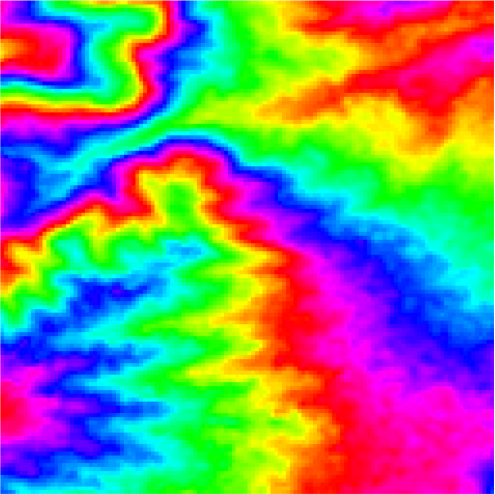
\includegraphics[width=0.40\linewidth]{original_phase}
     }
     \subfloat[Simulated InSAR Image with noise \label{fig:img_simulates_with_noise:b}]{%
       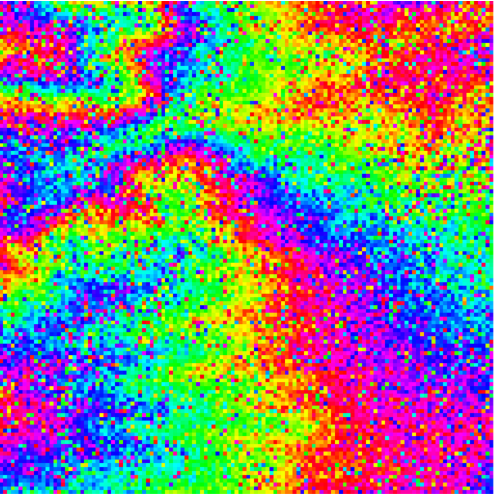
\includegraphics[width=0.40\linewidth]{noise_phase}
     }
\caption{Simulated interferometric phase images (a)~with, and (b)~without noise.}
     \label{fig:img_simulates} 
\end{figure}

\subsubsection{La Cumbre Volcano InSAR Image}\label{subsec:materials_la_cubre}
We analyzed data from the eruption of the La Cumbre volcano on Fernandina Island in the Galápagos archipelago, Ecuador, on January 12, 2020, see~\cite{pechnikovLaCumbre}.  The Region of Interest (ROI) of the InSAR image presented in Figure~\ref{fig:insar_la_cumbre_InSAR} has $346\times492$ pixels.

Figure~\ref{fig:insar_la_cumbre_optica} shows the optical image of the La Cumbre region. Although we did not work with optical images in this research, we know they can show the volcano's characteristics very well and emphasize mountain features. For example, Figure~\ref {fig:insar_la_cumbre_optica} shows that the ground is very sloped closer to the volcano, whereas farther from the volcano is a flat region. The advantage of InSAR images is that they allow us to estimate the volcano's slope and height. In this way, we can monitor several environmental hazards, such as landslide or lava-flow speeds after a volcanic eruption, among many possibilities. The authors emphasized that no coregistration of the images was performed.   

\begin{figure}[hbt]
\centering
	\subfloat[InSAR Image\label{fig:insar_la_cumbre_InSAR}]{
		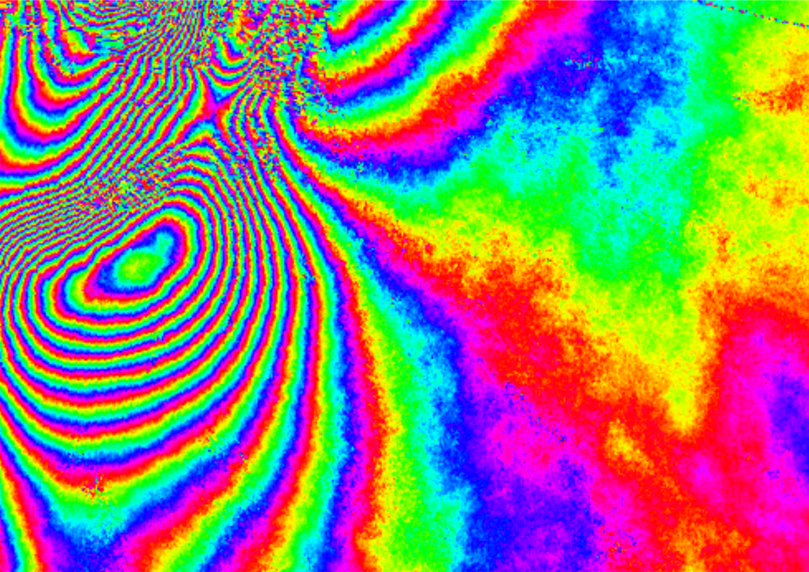
\includegraphics[width=0.5\linewidth]{interferograma_LaCumbe.pdf}}
	\subfloat[Optical Image\label{fig:insar_la_cumbre_optica}]{
		%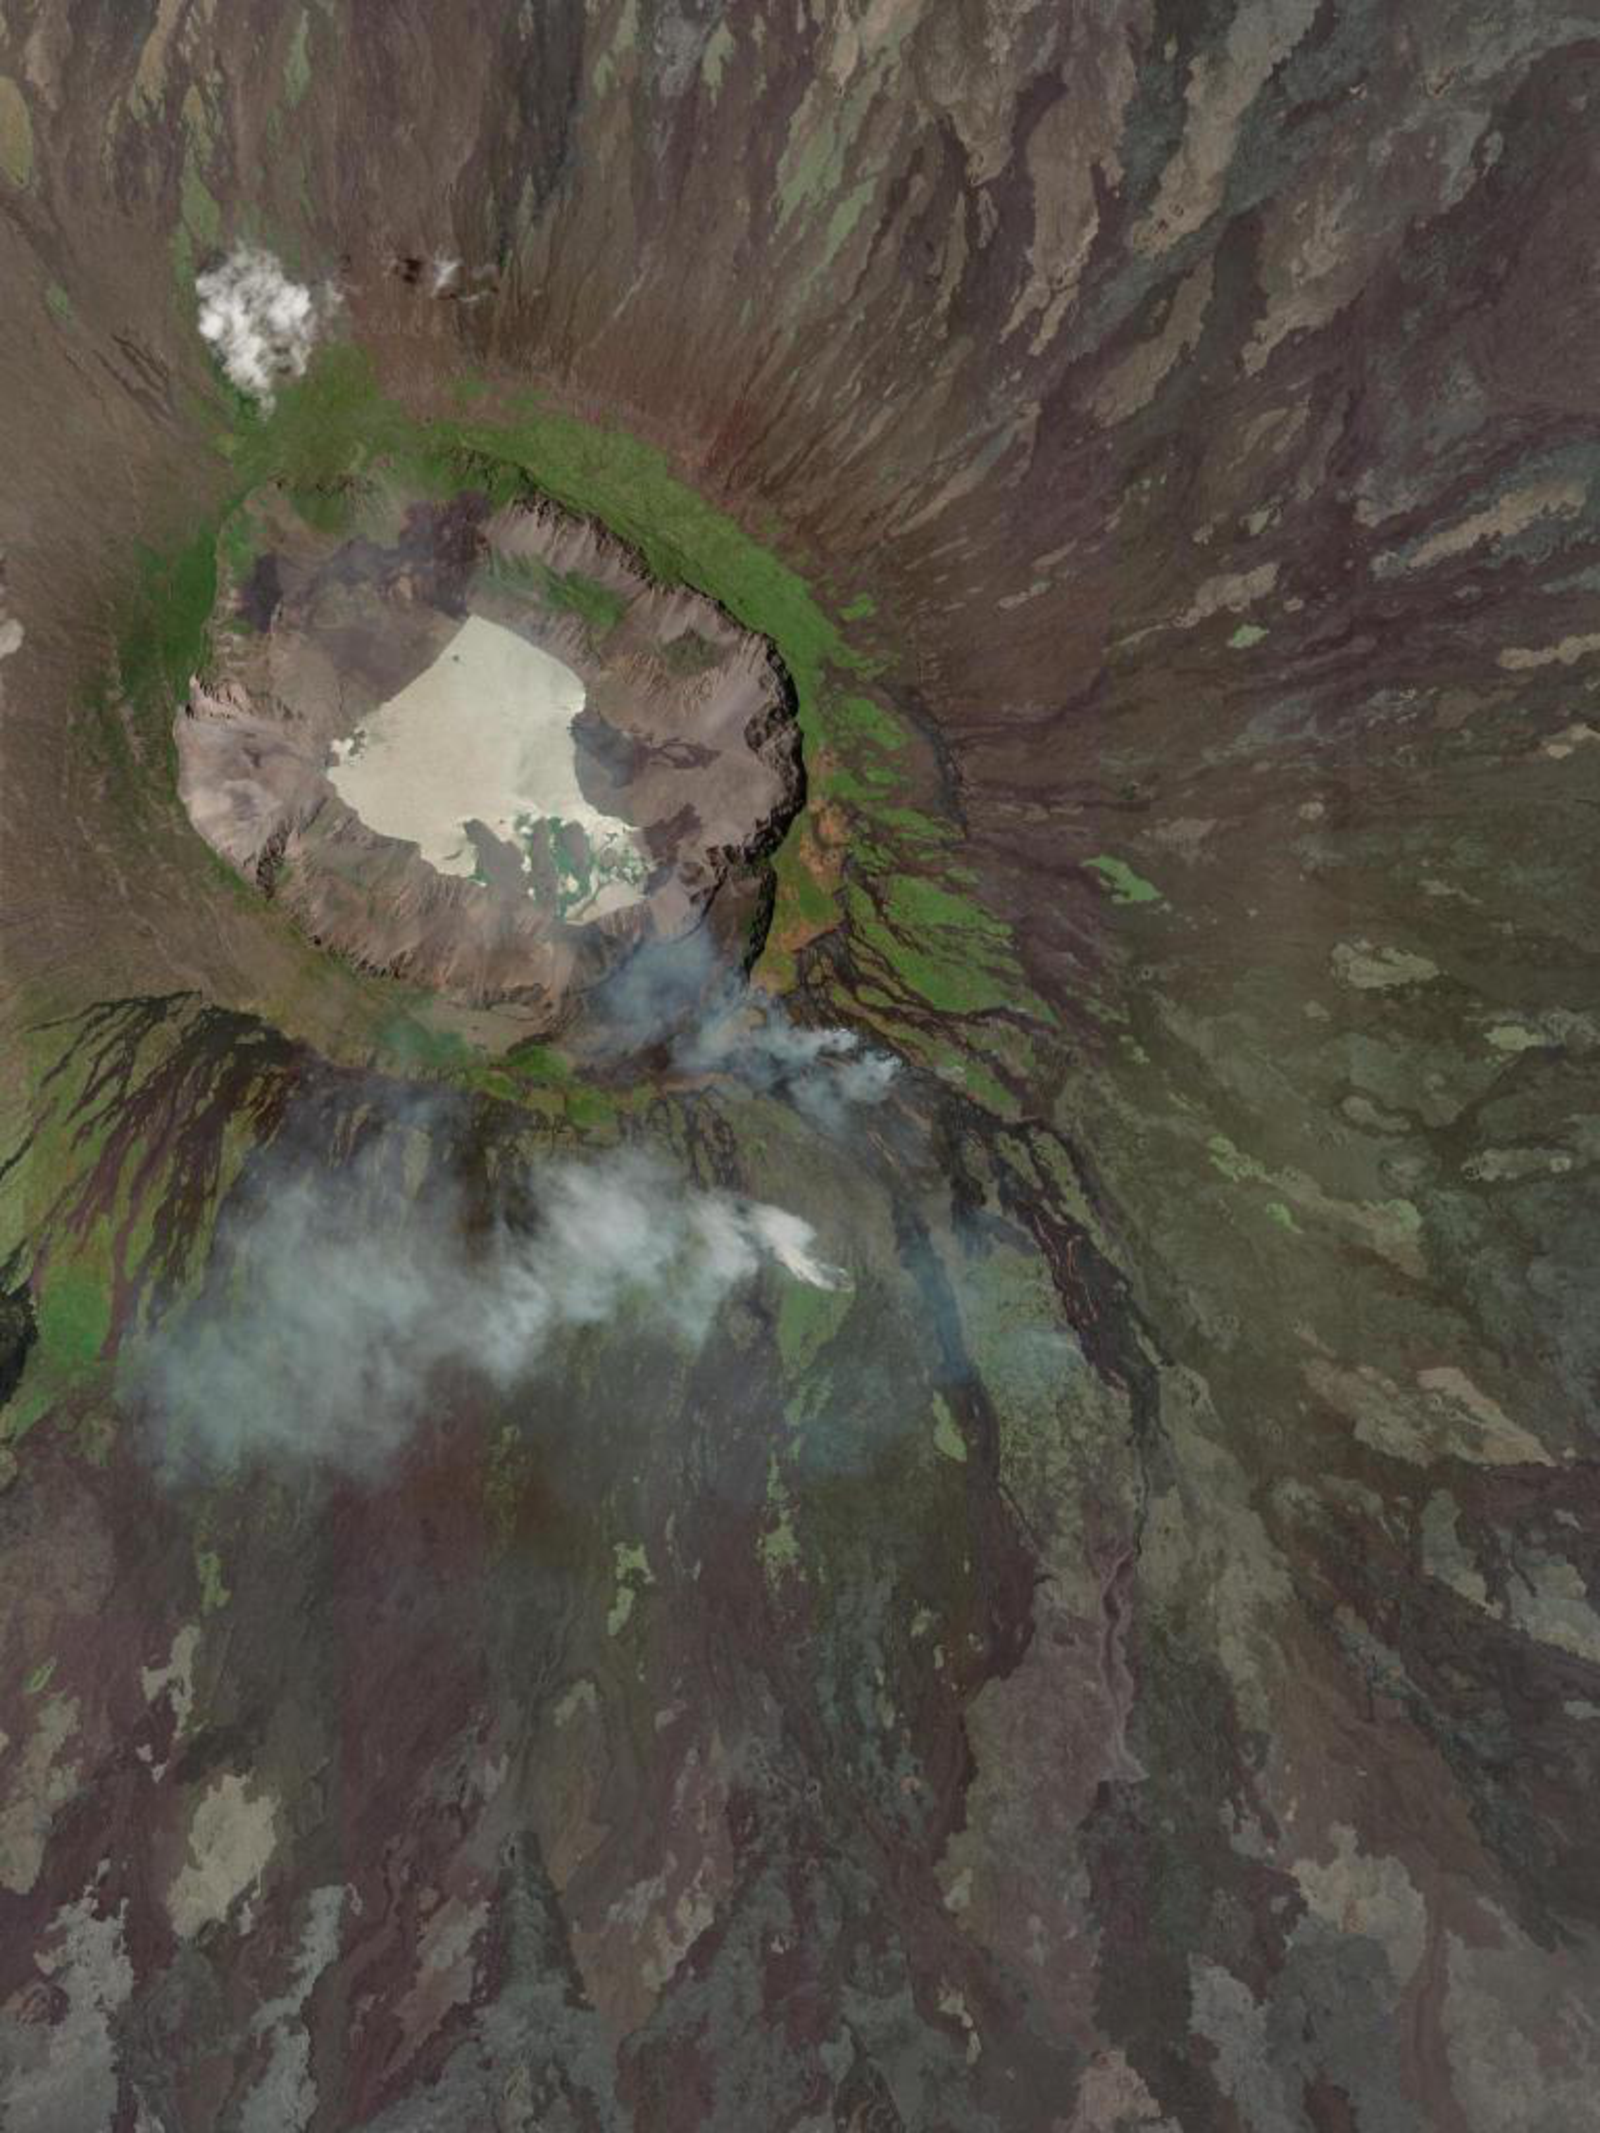
\includegraphics[width=0.265\linewidth]{la_cumbre_high_res.pdf}}
		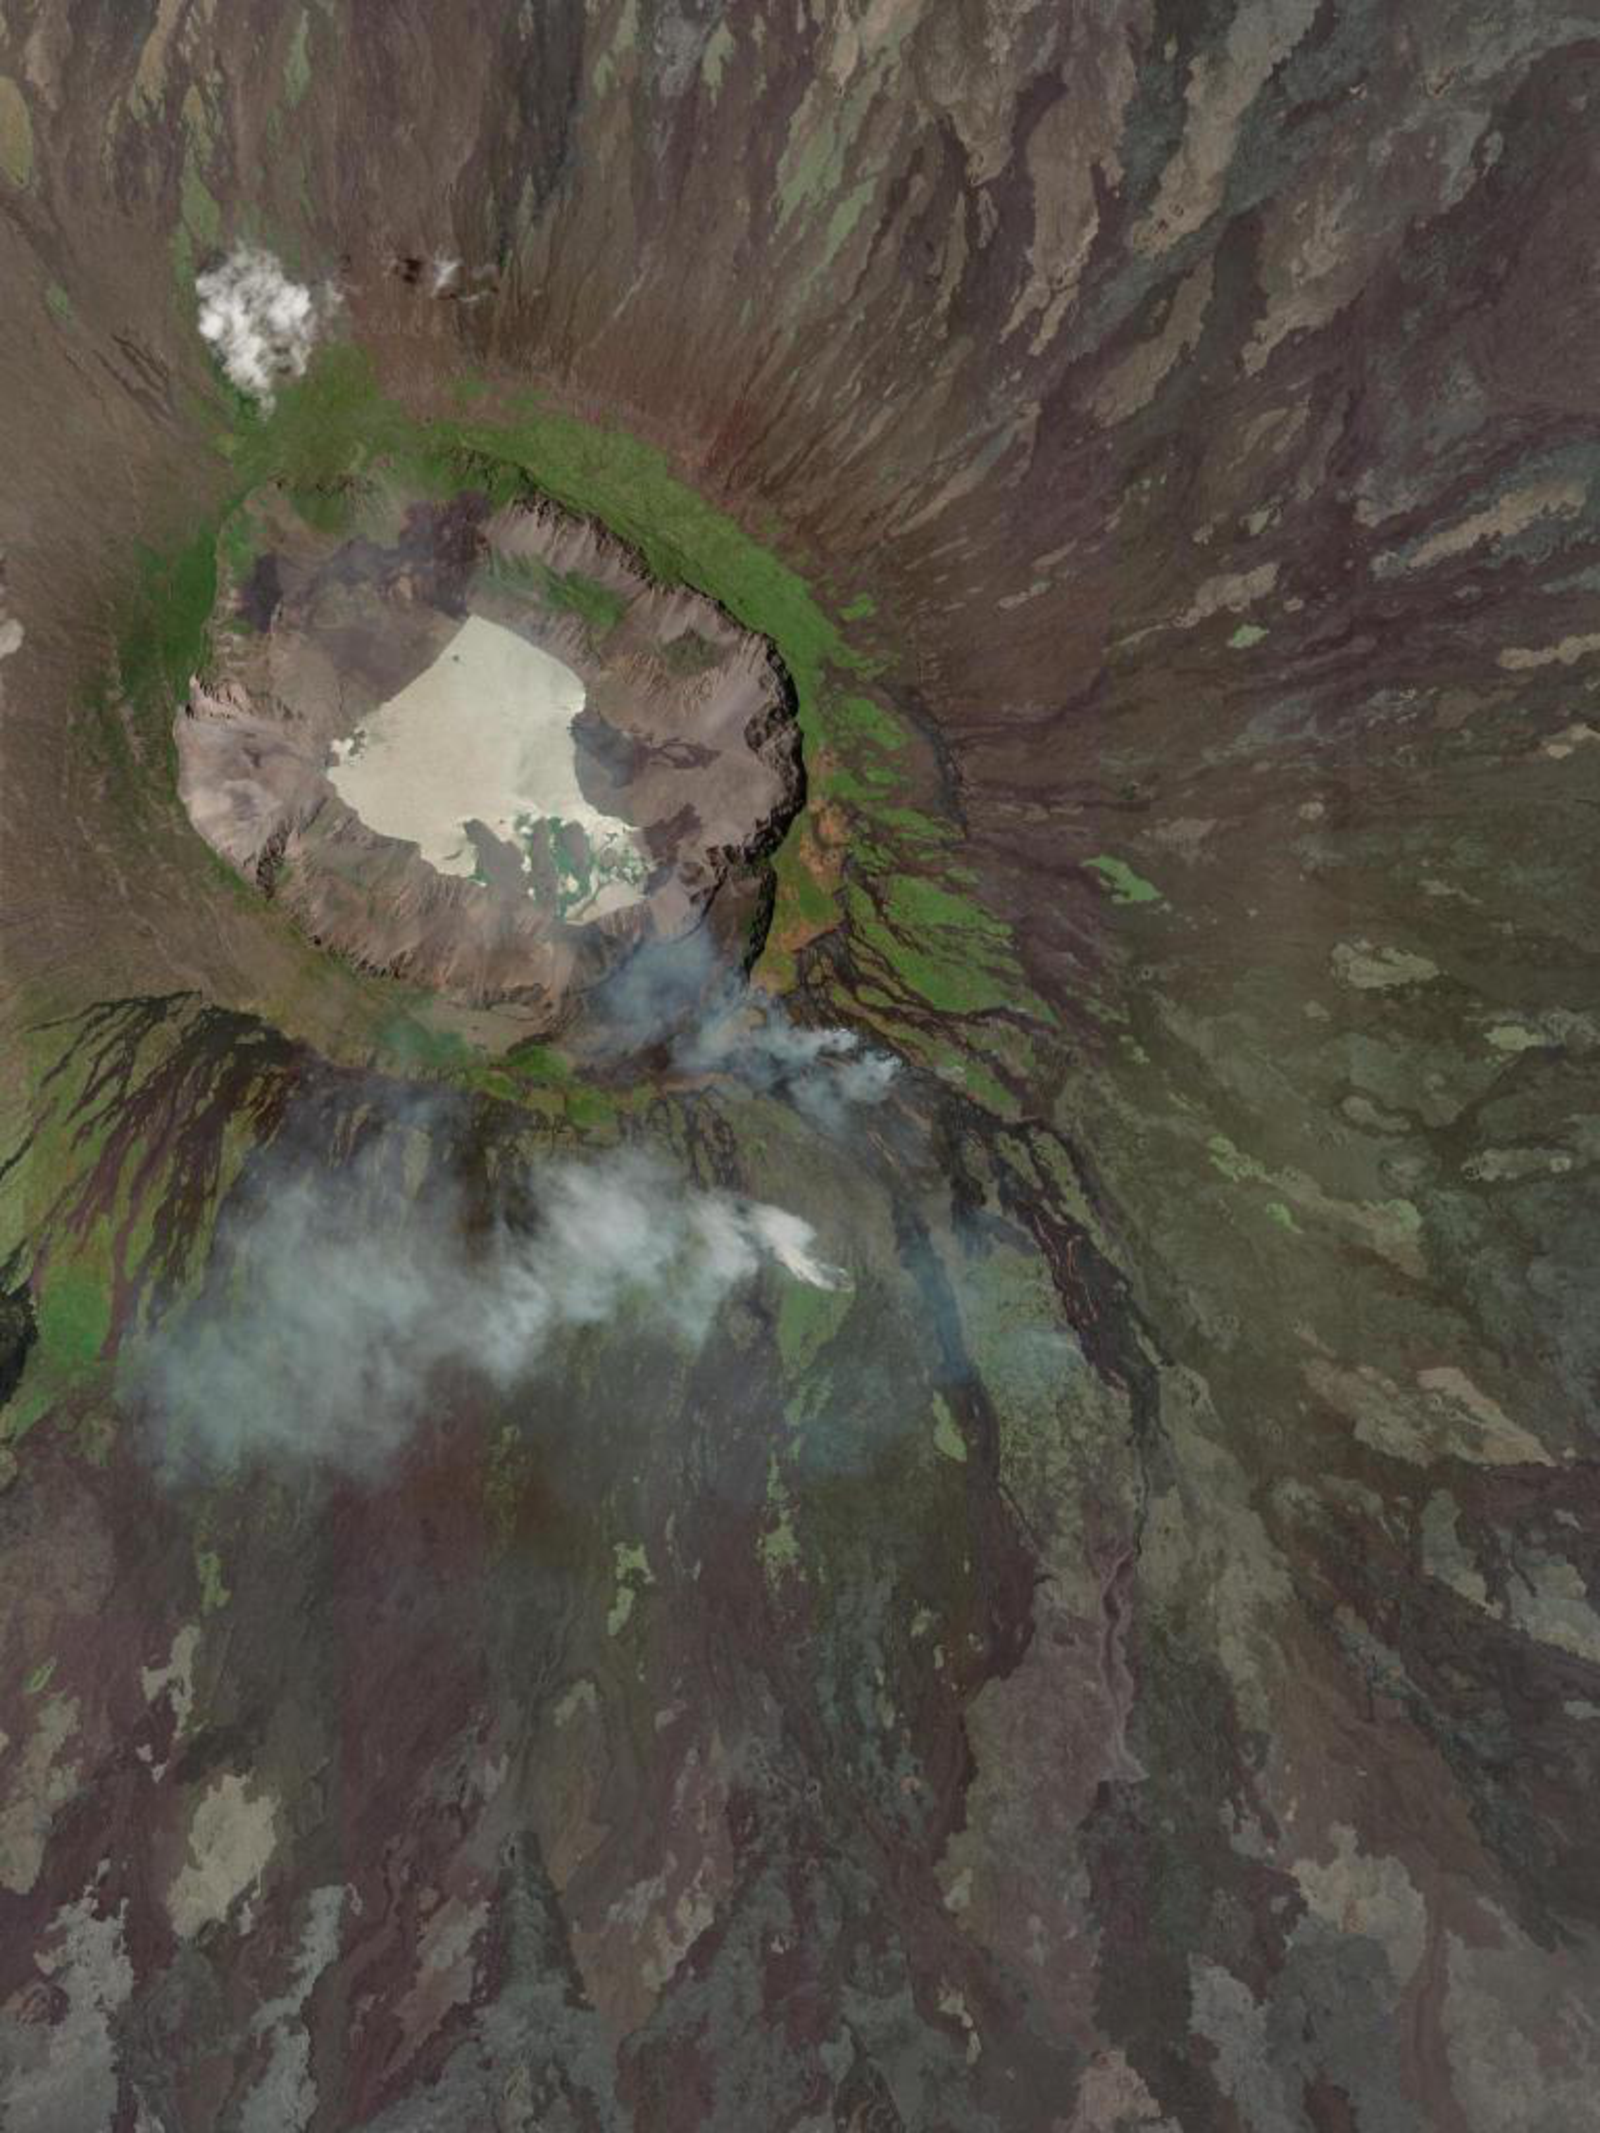
\includegraphics[width=0.48\linewidth, height=4.89cm]{la_cumbre_high_res.pdf}}
	\caption{La Cumbre Volcano Images}
	\label{fig:insar_la_cumbre}
\end{figure}


\subsubsection{Los Alamos InSAR Image}\label{subsec:materials_los_alamos}

Figure~\ref{fig:insar_uavsar_los_alamos} shows the InSAR image of Los Alamos, USA, to the left, while the right image is the region of interest (ROI) that we use for testing.


\begin{figure}[hbt]    
	\centering
      %   \subfloat[Los Alamos InSAR Image \label{fig:insar_uavsar_los_alamos:a}]{%
%       \includegraphics[width=0.52\linewidth]{arquivo_fix_alamos.pdf}
		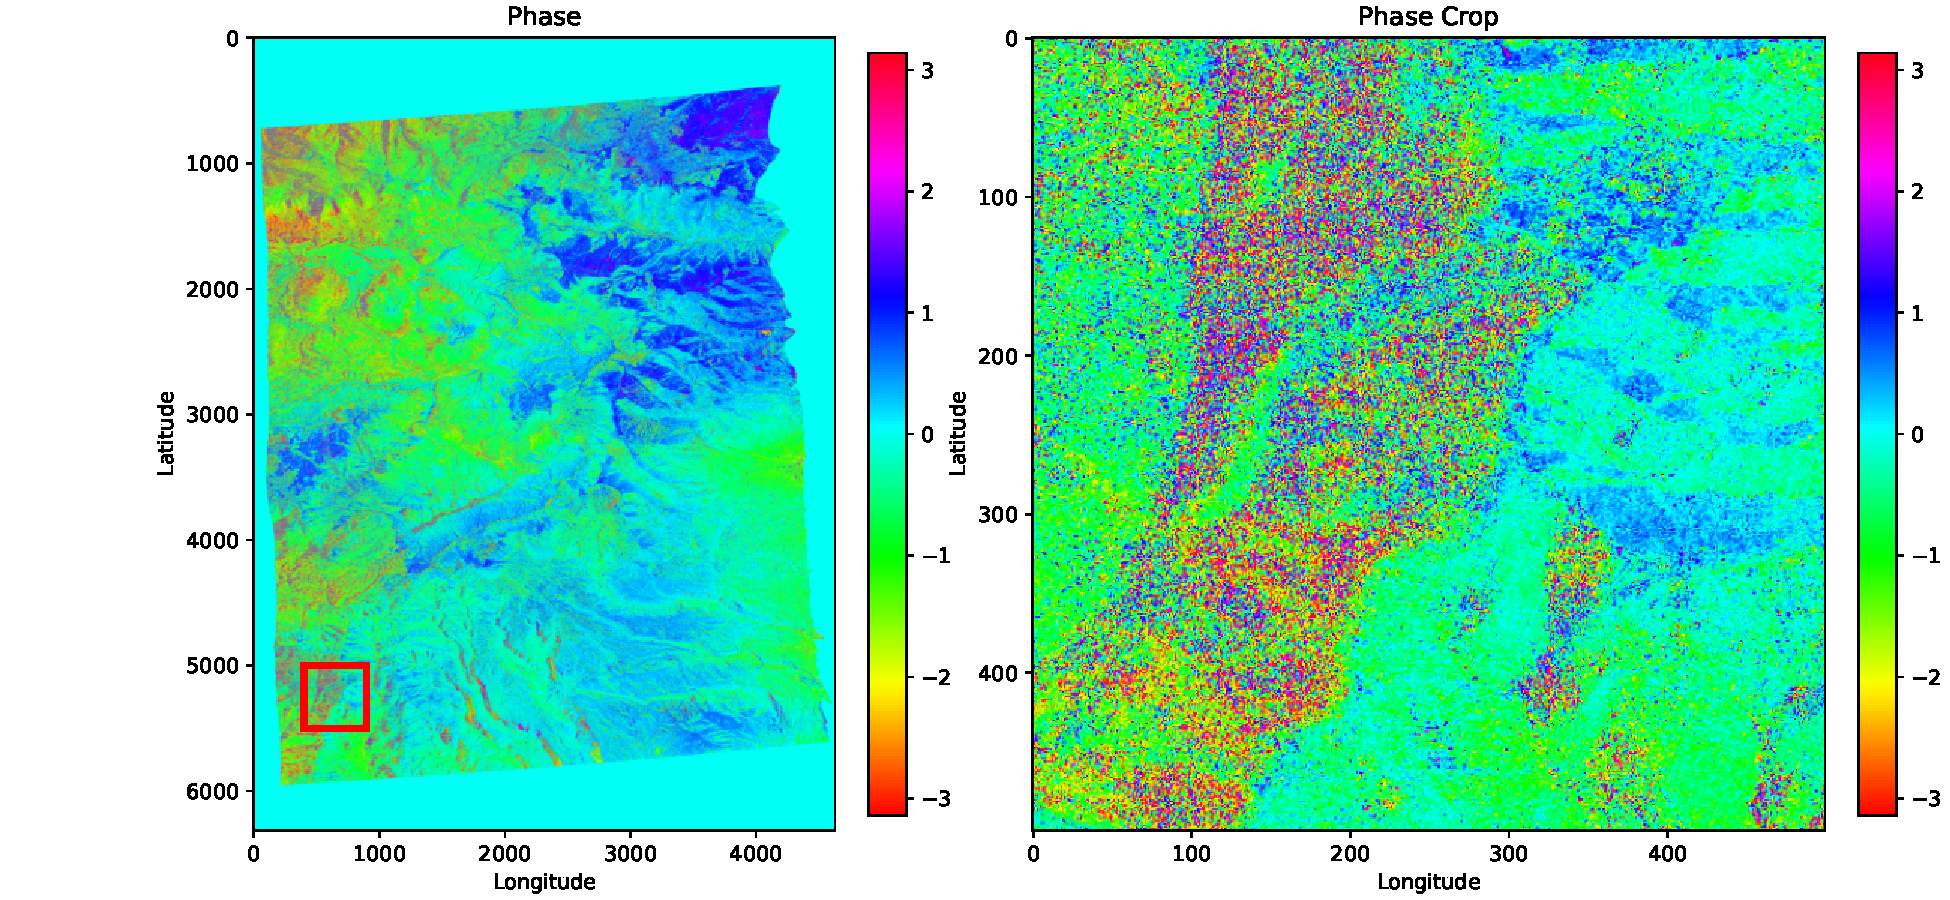
\includegraphics[width=1.0\linewidth]{los_alamos_orig_and_crop_500}
     %}
    \caption{Interferometric phase images acquired by the UAVSAR sensor: (a) Los Alamos, USA; (b) Los Alamos ROI .}
     \label{fig:insar_uavsar_los_alamos} 
\end{figure}

\subsubsection{Robledo Volcano InSAR Image}\label{subsec:materials_robledo}

%From the same source, we obtained the Robledo Volcano InSAR image, Argentina. 
Figure~\ref{fig:insar_uavsar_robledo} shows the InSAR image of Robledo Volcano, Argentina, to the left, while the ROI is shown to the right.


\begin{figure}[hbt]
    %\centering
     %\subfloat[Robledo Volcano InSAR Image  \label{fig:insar_uavsar_robledo:b}]{%
%       \includegraphics[width=0.51\linewidth]{arquivo_fix_robledo.pdf}
       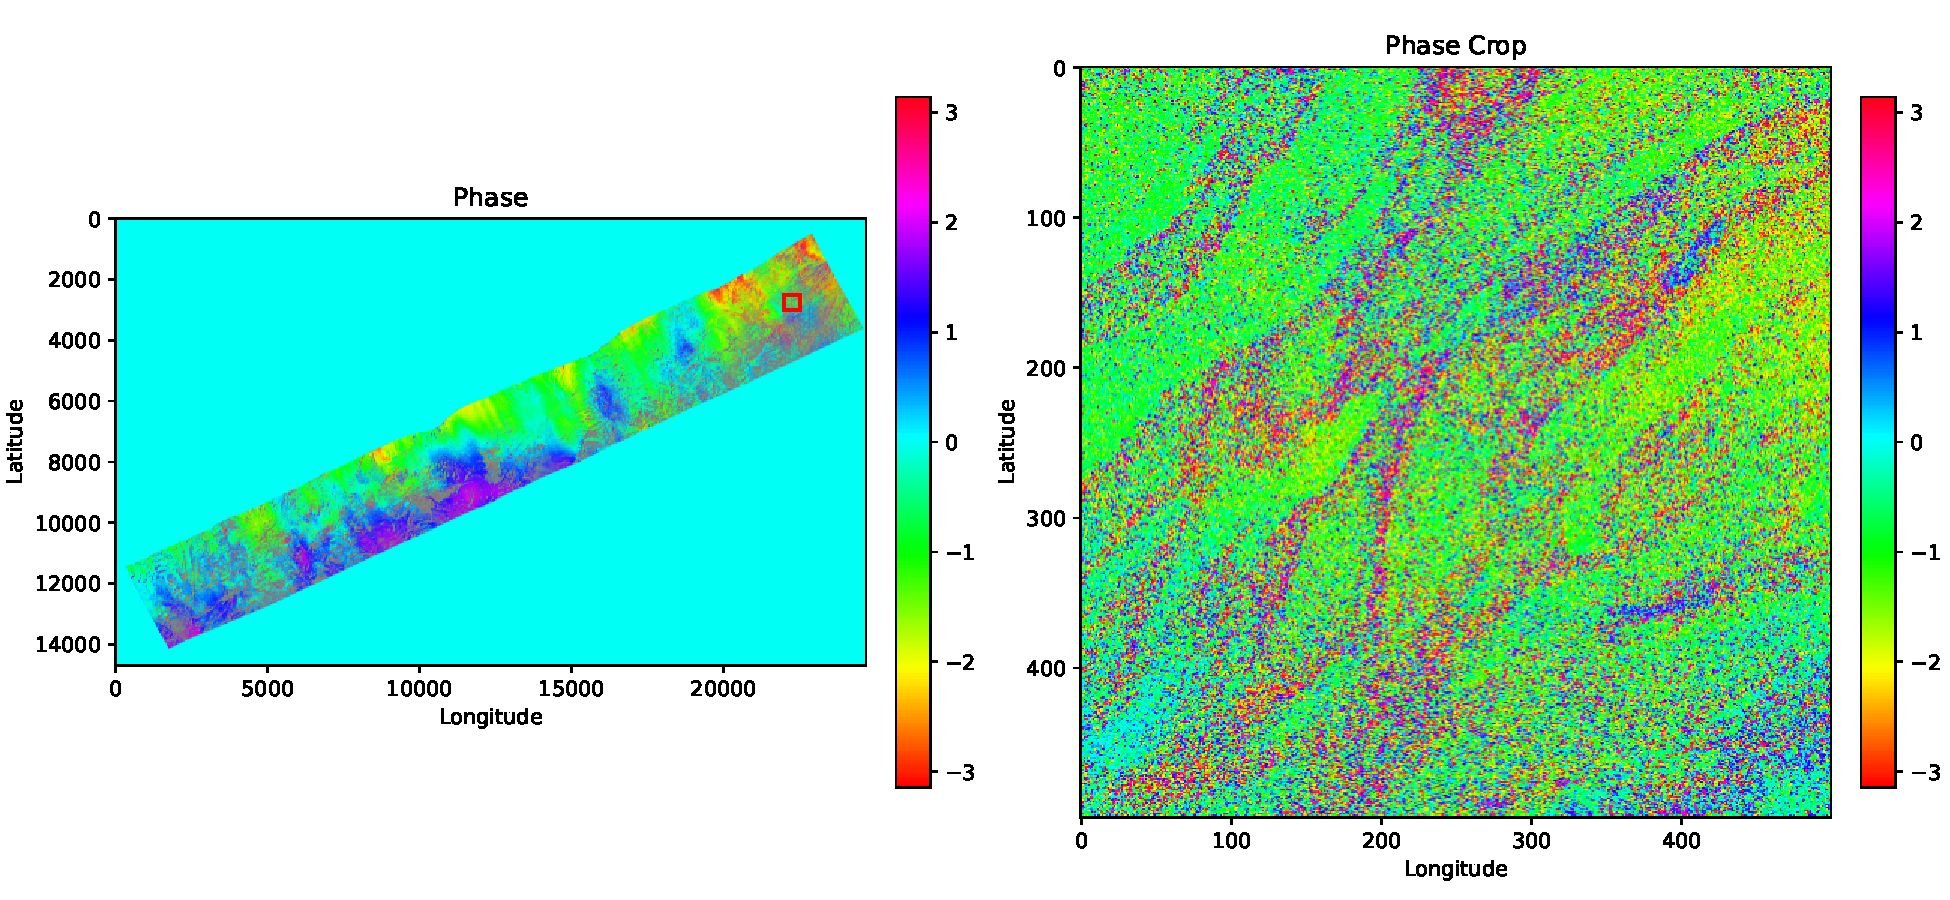
\includegraphics[width=1.0\linewidth]{robledo_orig_and_crop_500}
     %}
    \caption{Interferometric phase images acquired by the UAVSAR sensor: (a) Robledo Volcano, Argentina; (b) Robledo ROI}
     \label{fig:insar_uavsar_robledo} 
\end{figure}
\newpage

Table~\ref{tab:uavsar_charac} presents the main image acquisition characteristics of these InSAR images. 

\begin{table}[hbt]
	\caption{Image Characteristics.\label{tab:uavsar_charac}}
	\begin{tabularx}{\textwidth}{
			l % Filter name
			>{\centering\arraybackslash}X % Number of Residues
			>{\centering\arraybackslash}X % Reduction of residues (%)
			>{\centering\arraybackslash}X % RT (s)
		}
		\toprule
		\textbf{Images}&\textbf{\makecell{La Cumbre}} & \textbf{\makecell{Los Alamos}} & \textbf{\makecell{Robledo}}  \\
		\midrule
		Sensor                &   Sentinel-1          & UAVSAR                         & UAVSAR\\
		Band                  &  C--band              & L--band                        & L--band \\
		Resolution            & \qty{15}{\metre}      & \qty{6}{\metre}                & \qty{6}{\metre} \\
		Date of Acquisition   & 12-Jan-2020           &  19 and 26-Feb-2020            & 24-Mar-2013 and 29-Apr-2014  \\
		Dimension             & $972\times 920$       & $6315\times 4631$              & $14702\times 24680$  \\
		ROI                   & $346\times492$        & $500\times 500$                & $500\times 500$  \\
		(Lat, Lon)            & (\qty{-91.53}{\degree}, \qty{-0.37}{\degree})       & (\qty{36.03}{\degree}, \qty{-106.4}{\degree})                & (\qty{-26.6}{\degree}, \qty{-67.52}{\degree})\\
		Bandwidth             & \qty{80}{\mega\hertz} &  \qty{80}{\mega\hertz}         & \qty{80}{\mega\hertz}\\
		Wavelength            &\qty{5.6}{\centi\metre} & \qty{23.84}{\centi\metre} &\qty{23.84}{\centi\metre} \\
		Pulse Length          &  --                   & \qty{40}{\micro\second}        & \qty{40}{\micro\second} \\
		Sensor Altitude (avg) &  --                   &  \qty{12494.7061}{\meter}      & \qty{12495.2486}{\meter}\\           
		\bottomrule
	\end{tabularx}
\end{table}

\subsubsection{Computational Resources}\label{subsec:Computational_Resources}

We performed the experiments presented in this work in an Intel(R) Core i5-8265U CPU  \qty{1.6}{\giga\hertz} computer with \qty{4.0}{\giga\byte} of RAM running Windows 10 Pro 64 bits. 
All the coding was performed using the R language. 
The codes and data are available at~\url{https://github.com/araujoUFPE}, except the images of Los Alamos and Robledo Volcano available in~\url{http://uavsar.jpl.nasa.gov/}.

\subsection{Methods}\label{subsec:methods}

%This section presents the concepts and definitions of probability distributions, including both physical and empirical approaches, as well as their applications in the context of circular data.
Interferometric data (phases) are angular variables defined on the circle, with support in the interval $(-\pi, \pi]$ and periodicity $2\pi$. 
Thus, the probability density functions that form the basis of this work, particularly the physical models described in expressions~\eqref{subsec:sec3.2.1_cap3Eq7} and~\eqref{subsec:sec3.2.1_cap3Eq8}, are circular distributions. 

%To properly understand these models, this section begins with a review of the basic concepts of circular statistics (section~\ref{subsec:models}), discusses the construction of distributions with circular support (section~\ref{subsec:circulars_models}), and presents classical models widely used in the literature (section~\ref{models_classic}), such as the uniform circular, von Mises, cardioid, and wrapped versions of continuous distributions. 
%In addition to providing the theoretical foundation necessary for the modeling adopted in this study, this section aims to contextualize the classical models that serve as references for both empirical constructions and the development of new filtering algorithms.

Circular data arise in a wide range of research fields~\cite{OneDirection?ATutorialforCircularDataAnalysisUsingRWithExamplesinCognitivePsychology}, ranging from ecology to medical sciences. 
It is common to specify a circular distribution as that of a random angle, which we denote by $\Theta$, corresponding to a point on the circumference of the unit circle~\cite{CircularStatisticsinR}. 
To handle this type of data, it is necessary to use probabilistic models that account for the cyclic structure, allowing for proper analysis and interpretation of the results.

\subsubsection{Empirical Circular Models}\label{subsec:circulars_models}

%Several methods can be employed to obtain circular distributions. 
%According to \citet{CircularStatisticsinR}, perhaps the simplest is perturbation: the density of an existing circular distribution is multiplied by a suitably chosen function, resulting in a product that is also a circular density. 
%As an example of this type of construction, we can highlight the cardioid model presented in section~\ref{sec:sec3.1.2_cap3}.

A classical approach to obtaining circular distributions is wrapping.
It consists of adapting a continuous distribution with support on the real line to the interval $(-\pi, \pi]$ or $[0, 2\pi)$. 
This approach transforms the original variable into a circular one through the modulo $2\pi$ operation, ensuring the periodicity of the resulting density. 
The Wrapped Normal and Wrapped Cauchy models, discussed below, are examples of this type of construction. 
In this study, we adopt the interval $(-\pi, \pi]$ as the support for circular models. 
%For more information on this technique, see~\cite{TopicsinCircularStatistics} and~\cite{CircularStatisticsinR}.

%In contrast to approaches based on adapting distributions defined on the real line, the direct construction of circular distributions aims to formulate models already defined on the circle, without the need to alter the original support~\cite{CircularStatisticsinR}. Classic examples of this approach include the uniform circular distribution (section~\ref{sec:sec3.1.1_cap3}) and the von Mises distribution (section~\ref{sec:sec3.1.3_cap3}). The latter was introduced by von Mises in 1918 to study deviations of measured atomic weights from integer values. According to~\cite{StatisticsofDirectionalData}, the von Mises model plays a fundamental role in statistical inference on the circle, holding a position analogous to that of the normal distribution.

%It is worth noting that, in the literature, the density and distribution functions presented below are generally defined on the interval $[0, 2\pi)$\cite{TopicsinCircularStatistics},\cite{MARDIA2006}, and~\cite{CircularStatisticsinR}. 
%This transformation is particularly useful in applications involving interferometric data, where it is convenient to represent phases within an interval centered at the origin. 
%To this end, we assume that an angle $\theta \in [0, 2\pi)$ can be equivalently represented in the interval $(-\pi, \pi]$, as defined below:
%\begin{equation}
%	\theta' =
%	\begin{cases}
%		\theta, & \text{if}~~0 < \theta \leq \pi; \\
%		\theta - 2\pi, & \text{if}~~\pi < \theta < 2\pi; \\
%		-\pi, & \text{if}~~\theta = 0.
%	\end{cases}
%\end{equation}
%
%Alternatively, we can write:
%\begin{equation}\label{mod}
%	\theta' = \left((\theta + \pi) \bmod 2\pi\right) - \pi.
%\end{equation}
%
%The expression in~\eqref{mod} can be interpreted in three steps: (i) we add $\pi$ to the value of $\theta$, aiming to center the interval around zero; (ii) we apply the modulo $2\pi$ operator, ensuring the periodicity of the function; and (iii) we subtract $\pi$, to obtain the final value within the desired interval $(- \pi, \pi]$.
%
%\subsubsection{Classical Circular Models}\label{models_classic}


%Let $\Theta$ be a Circular Random Variable (CRV), that is, a variable taking values in the interval $(- \pi, \pi]$ with periodicity $2\pi$. In the following sections, some classical models dealing with angular data are presented~\cite{TopicsinCircularStatistics, CircularStatisticsinR}.

\subsubsubsection{Circular Uniform Distribution}\label{sec:sec3.1.1_cap3}

The probability density function of the Circular Uniform Distribution (CUD) is:
\begin{eqnarray}\label{sec:sec3.1.1_cap3Eq1}
	f_{\Theta}(\theta)=\frac{1}{2\pi}~~\text{for}~~-\pi<\theta\leq\pi.
\end{eqnarray}
This model is relevant when analyzing circular data because it reflects the absence of a preferred direction, and appears as a limit law for the two models discussed in the following.

\subsubsubsection{Wrapped Normal Distribution}%\label{sec:sec3.1.4_cap3}

The Wrapped Normal (WN) distribution is a symmetric two-parameter distribution that can be obtained by wrapping the Normal distribution with mean $\mu$ and variance $\sigma^2$ around the unit circle. 
The probability density function that characterises the WN distribution~\cite{TopicsinCircularStatistics, CircularStatisticsinR, EfficientEvaluationoftheProbabilityDensityFunctionofaWrappedNormalDistribution} is:
\begin{equation}\label{sec:sec3.1.4_cap3Eq1}
	f_{\Theta}(\theta; \mu, \sigma^2) = \frac{1}{\sigma\sqrt{2\pi}}\sum_{k=-\infty}^{\infty}\exp\left[-\frac{(\theta-\mu+2k\pi)^2}{2\sigma^2}\right], \text{ for }-\pi < \theta \leq \pi,
\end{equation}
with location parameter $\mu \in (-\pi, \pi]$ and scale parameter $\sigma > 0$.

The terms of the series in~\eqref{sec:sec3.1.4_cap3Eq1} decay exponentially and tend to zero. 
%This occurs because, due to the nature of the Gaussian distribution, the contribution of each term decreases rapidly as $k$ increases. 
Therefore, for large values of $k$, the terms become practically negligible, allowing the probability density function to be approximated by a truncated series~\cite{EfficientEvaluationoftheProbabilityDensityFunctionofaWrappedNormalDistribution}: 
\begin{equation}	f_{\Theta}(\theta; \mu, \sigma^2)
	\approx f_n(\theta; \mu, \sigma^2) 
	=\frac{1}{\sigma\sqrt{2\pi}}\sum_{k=-n}^{n}\exp\left[-\frac{(\theta-\mu+2k\pi)^2}{2\sigma^2}\right], \text{ for }-\pi < \theta \leq \pi, \label{sec:sec3.1.4_cap3Eq1.1}
\end{equation}
in which only $2n + 1$ terms of the sum are considered. An alternative and more useful form to represent the density in~\eqref{sec:sec3.1.4_cap3Eq1.1} is presented by~\cite{CircularStatisticsinR, EfficientEvaluationoftheProbabilityDensityFunctionofaWrappedNormalDistribution} and expressed as:
\begin{equation}\label{sec:sec3.1.4_cap3Eq2}
	g_{\Theta}(\theta; \mu, \rho)=\frac{1}{2\pi}\left(1+2\sum_{k=1}^{\infty}\rho^{k^2}\cos k(\theta-\mu) \right), \text{ for } -\pi < \theta \leq \pi,
\end{equation}
where $\rho = \exp(-\sigma^2/2)$. Analogous to~\eqref{sec:sec3.1.4_cap3Eq1.1}, we define a truncated version of the density in~\eqref{sec:sec3.1.4_cap3Eq2}, given by:
\begin{equation}\label{sec:sec3.1.4_cap3Eq2.1}
	g_{\Theta}(\theta; \mu, \sigma^2)
\approx g_n(\theta; \mu, \sigma^2) = \frac{1}{2\pi}\left(1+2\sum_{k=1}^{n}\rho^{k^2}\cos k(\theta-\mu) \right), \text{ for }-\pi < \theta \leq \pi.
\end{equation}

The parameter $n$, both in $f_n$ and $g_n$, is treated in the same way.
However, evaluating $f_n$ involves $2n + 1$ terms in the sum, while evaluating $g_n$ involves only $n$ terms~\cite{EfficientEvaluationoftheProbabilityDensityFunctionofaWrappedNormalDistribution}. 
We observe that as $\rho\rightarrow0$, the WN distribution converges to the circular uniform distribution.

%\begin{enumerate}[label=\alph*)]
%\item   - 
%
%\item \label{sec:sec3.1.2_cap3} Cardioid Distribution - 
%The Cardioid Distribution (CD), derived from the cardioid curve, has a probability density function defined by~\cite{TopicsinCircularStatistics},~\cite{CircularStatisticsinR},~\cite{GeneralizedCardioidDistributionsforCircularDataAnalysis}:
%\begin{eqnarray}\label{sec:sec3.1.2_cap3Eq1}
%	f_{\Theta}(\theta; \mu, \rho)=\frac{1}{2\pi}\{1+2\rho\cos(\theta-\mu)\}~~\text{for}~~-\pi<\theta\leq\pi.
%\end{eqnarray}
%where $-\pi < \mu \leq \pi$ is the mean direction and $|\rho| \leq 0.5$ is the concentration parameter, indicating the dispersion of the circular data around the mean direction. The CD is unimodal and symmetric about the mean $\mu$. Integrating the model in~\eqref{sec:sec3.1.2_cap3Eq1}, we obtain the CDF, defined by:
%\begin{equation}
%	F_{\Theta}(\theta; \mu, \rho) = \frac{\theta+\pi}{2\pi} + \frac{\rho}{\pi} \left[\left( \sin(\theta - \mu) - \sin \mu \right) \right]~~\text{for}~~-\pi<\theta\leq\pi.
%\end{equation}
%
%\item \label{sec:sec3.1.4_cap3} Wrapped Normal Distribution - 

%
%\item  Wrapped Cauchy Distribution - 
\subsubsubsection{Wrapped Cauchy Distribution}\label{sec:sec3.1.5_cap3}

The Wrapped Cauchy (WC) distribution is characterised by the probability density function:
\begin{equation}\label{sec:sec3.1.5_cap3Eq2}
	f_{\Theta}(\theta;\mu,\rho) = \frac{1}{2\pi} \frac{1-\rho^2}{1+\rho^2-2\rho\cos(\theta-\mu)} ,
	\text{ for }-\pi < \theta \leq \pi,
\end{equation}
where $\rho = e^{-\sigma} \in [0, 1]$.
As previously observed for the WN distribution, when $\rho \rightarrow 0$, the WC converges to the circular uniform distribution~\cite{CircularStatisticsinR}.
%
%\item \label{sec:sec3.1.3_cap3} von Mises Distribution - 
%The von Mises (VM) distribution, also known as the Circular Normal distribution, has a probability density function~\cite{TopicsinCircularStatistics},~\cite{CircularStatisticsinR}, given by:
%\begin{eqnarray}\label{sec:sec3.1.3_cap3Eq1}
%	f_{\Theta}(\theta; \mu, \kappa) = \frac{1}{2\pi I_0(\kappa)} e^{\kappa\cos(\theta - \mu)},~~\text{for}~~-\pi < \theta \leq \pi,
%\end{eqnarray}
%where $\kappa \geq 0$ is the concentration parameter, $-\pi < \mu \leq \pi$ is the location parameter or mean angle, and $I_0(\kappa)$ is the modified Bessel function of the first kind of order zero~\cite{KATO2010}, which is defined by:
%\begin{eqnarray}\label{sec:sec3.1.3_cap3Eq2}
%	I_0(\kappa) = \frac{1}{2\pi} \int_{-\pi}^{\pi} e^{\kappa\cos\theta} d\theta = \sum_{r=0}^{\infty} \left( \frac{\kappa}{2} \right)^{2r} \left( \frac{1}{r!} \right)^2.
%\end{eqnarray}
%
%In this model, we can observe that when $\kappa = 0$, the VM reduces to the circular uniform distribution over the interval $(-\pi, \pi]$, regardless of the value of $\mu$, for more information on the properties of the von Mises distribution, see~\cite{DirectionalStatistics, TopicsinCircularStatistics, KATO2010} and~\cite{CircularStatisticsinR}. Although the classical circular models mentioned in this section are not directly employed in the filters developed in this work, their presentation is relevant to establish the main modeling approaches for angular data, such as the phase in interferometric images. Next, we address the physical and empirical models actually used in the filtering algorithms proposed in this study.
%\end{enumerate}

\subsubsection{Physical Models}\label{subsec:physical_model_pd}

Using a physically-based approach, 
Lee et al.~\cite{IntensityAndPhaseStatisticsOfMultilookPolarimetricAndInterferometricSARimagery} derived a physical model for the phase difference. 
The probability density function (PDF) is expressed as follows:
\begin{equation}\label{subsec:sec3.2.1_cap3Eq7}
	f(\psi; \theta, \rho_c, L)=\frac{\Gamma(L+\frac{1}{2}) (1-|\rho_c|^2)^L\beta}{2\sqrt{\pi}\Gamma(L)(1-\beta^2)^{L+\frac{1}{2}}}
	+\frac{(1-|\rho_c|^2)^L}{2\pi} {_2} F_1 \Big(L,1;\frac{1}{2};\beta^2\Big),
\end{equation}
% AAB - Não foi definido o L e a função gamma ($\Gamma$), como tem espaço pode dizer que é a função Gamma.
%%% JEA corrigido
where $-\pi<\psi\leq\pi$ is the phase,
$\rho_c$ is the complex correlation coefficient, 
$\beta=|\rho_c|\cos(\psi-\theta)$, $L$ is the number of looks, 
$\theta$ is the phase between channels, $\Gamma$ is the gamma function and
${_2}F_1$ is the Gauss Hypergeometric Function (GHF).

The authors provided~\eqref{subsec:sec3.2.1_cap3Eq7} for $L=1,2,3,4$ using Gauss' recurrence formulas. 
Because of the dependency on the GHF, computing and analyzing the statistical properties of~\eqref{subsec:sec3.2.1_cap3Eq7} is challenging or even unmanageable for a significant number of looks or high correlation values~\cite{FastandAccurateComputationoftheMultilookInterferometricPhaseProbabilityDensityFunction,GaussianApproximationofIinterferometricPDFforMLEderivation}.

To solve this problem, Gierull~\cite{ClosedFormExpressionsforInSARSampleStatisticsandItsApplicationtoNonGaussianData} proposed a new form of equation~\eqref{subsec:sec3.2.1_cap3Eq7} restricting the number of looks to positive integers greater than $1$; this constraint makes the model numerically tractable. 
The probability density function becomes:
\begin{multline}\label{subsec:sec3.2.1_cap3Eq8}
	f(\psi; \theta, \rho_c, L)
	=\frac{(1-\rho_c^2)^L}{2\pi\Gamma(L)(1-\beta^2)^{L+\frac{1}{2}}}\left\lbrace \sqrt{\pi}\Gamma\Big(L+\frac{1}{2}\Big)\beta\right.\\
	+\frac{\Gamma\big(L-\frac{1}{2}\big) }{\sqrt{\pi}}\bigg[ \sqrt{1-\beta^2}+2\Big(L-\frac{1}{2}\Big)\beta\arcsin\beta\bigg]\\ 
	\mbox{}+\sum_{k=1}^{L-1}\frac{(-1)^k}{2}\frac{\Gamma\big( k-L+\frac{1}{2}\big) \Gamma(L-k)}{\Gamma\big( \frac{3}{2}-L\big) }
	\left.\frac{1+(2k-1)\beta^2}{(1-\beta^2)^{k-L+\frac{1}{2}}}\right\rbrace.
\end{multline}

Eq.~\eqref{subsec:sec3.2.1_cap3Eq8} works around the numerical issues of the GHF function, however, it involves the gamma function, which can also bring significant numerical challenges.
Gierull~\cite{ClosedFormExpressionsforInSARSampleStatisticsandItsApplicationtoNonGaussianData} discusses strategies to circumvent the difficulties associated with large ratios from the last term in equation~\eqref{subsec:sec3.2.1_cap3Eq8}.
To solve these problems, Gierull uses the following relationship:
\begin{equation}\label{pro_log-gamma}
	\log\bigg[\frac{\Gamma(x+k)}{\Gamma(x+1)}\bigg]=\sum_{i=1}^{k-1}(x+k-i), \text{ for }x=\frac{1}{2}-L, \text{ and } k \text{ fixed}.
\end{equation}

\subsubsection{Comparing Physical Models}\label{subsec:lee_versus_gierull}

%Closed-form solutions for the expression in~\eqref{subsec:sec3.2.1_cap3Eq7}, when $L$ is a positive integer, were provided up to order $4$ by~\cite{IntensityAndPhaseStatisticsOfMultilookPolarimetricAndInterferometricSARimagery}, using Gauss recurrence formulas. For a larger number of looks, these solutions become lengthy and complicated at best. These challenges have motivated several authors to investigate approximate solutions~\cite{GaussianApproximationofIinterferometricPDFforMLEderivation,FastandAccurateComputationoftheMultilookInterferometricPhaseProbabilityDensityFunction,ClosedFormExpressionsforInSARSampleStatisticsandItsApplicationtoNonGaussianData} Gierull propose Eq.~\eqref{subsec:sec3.2.1_cap3Eq8}.
% coincides with~\eqref{subsec:sec3.2.1_cap3Eq7} for $L$ integer, but requires using $[L]$ otherwise. Moreover, for $L = 2$, these models share the same expression, defined by:

%We assess the impact of this approximation in Sec.~\ref{Sec:dKL-Lee-Gierull}.
%\begin{eqnarray}
%	f(\psi; \theta, \rho_c, 2)=\frac{3(1-|\rho_c|^2)^2\beta}{8(1-\beta^2)^{\frac{5}{2}}}+
%	\frac{(1-|\rho_c|^2)^2}{4\pi(1-\beta^2)^2}\cdot
%	\left(1+(1+\beta^2)+\frac{3\beta\arcsin\beta}{\sqrt{1-\beta^2}}\right) .
%\end{eqnarray}

Figure~\ref{eq_lee} illustrates the density function for phase differences according to the model proposed to ~\cite{IntensityAndPhaseStatisticsOfMultilookPolarimetricAndInterferometricSARimagery}, represented by expression~\eqref{subsec:sec3.2.1_cap3Eq7}, using actual values for the number of looks: $L=3.49$, $5.49$, $7.49$, and $9.49$, with $|\rho_c|=0.7$ and $\theta=0$. On the other hand, Figure~\ref{eq_gierull} shows the density function corresponding to the model proposed to~\cite{ClosedFormExpressionsforInSARSampleStatisticsandItsApplicationtoNonGaussianData}, according to expression~\eqref{subsec:sec3.2.1_cap3Eq8}, using integer values for the number of looks: $L=3$, $5$, $7$, and $9$, with parameters $|\rho_c| = 0.7$ and $\theta = 0$. We choose different multilook values $L$ for each model because these models share the same expression when $L$ is an integer.


Visually, we observe a small difference when comparing Figures~\ref{eq_lee} and~\ref{eq_gierull} for similar values of $L$, indicating that there is no significant loss of information when using model~\eqref{subsec:sec3.2.1_cap3Eq8} compared to the other model.
\begin{figure}[hbt]
	\subfloat[\centering Lee model Eq.~\eqref{subsec:sec3.2.1_cap3Eq7}\label{eq_lee}]{
		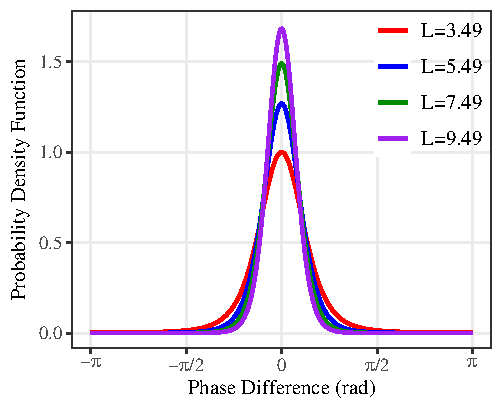
\includegraphics[width=.5\linewidth]{diff_phase_lee}}
	\subfloat[\centering Gierull model Eq.~\eqref{subsec:sec3.2.1_cap3Eq8}\label{eq_gierull}]{
		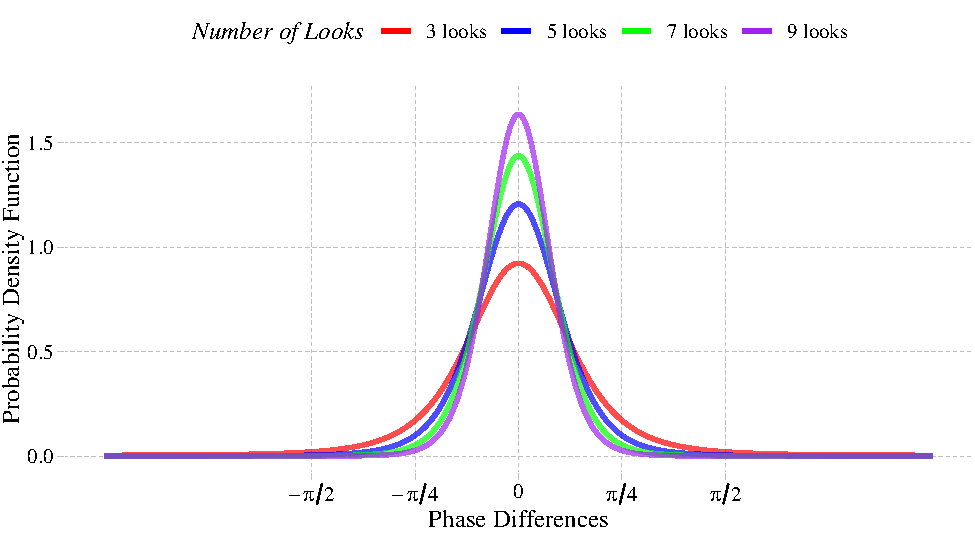
\includegraphics[width=.5\linewidth]{diff_phase_gierull}}
	\caption{\textmd{Comparison of Phase Difference PDFs: Lee versus Gierull models}}
	\label{ajuste_dKL_fisicos}
\end{figure}

%According to~\cite{ClosedFormExpressionsforInSARSampleStatisticsandItsApplicationtoNonGaussianData}, t
%The numerical instability associated with~\eqref{subsec:sec3.2.1_cap3Eq8} are related to the difficulty of directly computing the sum for large values of $L$ and/or coherence close to $1$.  
%These problems are overcome by using the log-gamma function, which allows adding or subtracting large exponentials instead of multiplying or dividing them.
%To apply~\eqref{pro_log-gamma} in Gierull's proposal density~\eqref{subsec:sec3.2.1_cap3Eq8} offers an elegant solution to avoid numerical issues when computing products or divisions of large quantities. 
%Figure~\ref{log_pdf_gierull} shows the approach applied to Gierull density performance with $\psi=\frac{\pi}{6}$, $L=1000$, and $\mid\rho_c\mid$ tends to 1, see~\cite{ClosedFormExpressionsforInSARSampleStatisticsandItsApplicationtoNonGaussianData}. It supports the equation proposed by Gierull in \eqref{pro_log-gamma}.
% AAB - Fazer uma figura equivalente no R seguindo o padrões do artigo. Basta pegar a gierull já programada e aplicar o log e ajeitar o plot.
%%% JEA Feito como sugerido
%\begin{figure}[hbt]
%	%\centering
%	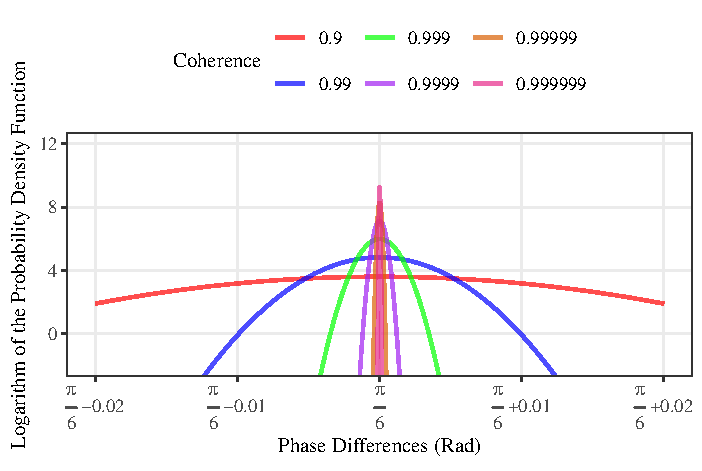
\includegraphics[width=.7\linewidth]{log_pdf_gierull_n1000_rho}
%	\caption{Logarithm of the Gierull interferometric phase pdfs for $L = 1000$ when $\rho$ tends to 1 centered at $\psi =\frac{\pi}{6} $}
%	\label{log_pdf_gierull} 
%\end{figure}

% For example, \textit{gamma(1000)/gamma(999)} in the language R results in \textit{NaN}. On the other hand, using \textit{exp(lgamma(1000) - lgamma(999))} yields $999$. Mathematically, the ratio \textit{A/B} can simply be expressed as \textit{exp(ln(A/B)) = exp(ln(A) - ln(B))}, which is computable when \textit{ln(A) - ln(B)} becomes a reasonable value. Moreover, \textit{lgamma(N)} and \textit{gamma(ln(N))} can be efficiently computed numerically without evaluating the gamma function itself. These were the reasons for using the \textit{ln} and \textit{exp} functions in the implementation of the model in~\eqref{subsec:sec3.2.1_cap3Eq8} in R.

%Closed-form solutions for the expression in~\eqref{subsec:sec3.2.1_cap3Eq7}, when $L$ is a positive integer, were provided up to order $4$ ($L = 1; 2; 3; 4$) by~\cite{IntensityAndPhaseStatisticsOfMultilookPolarimetricAndInterferometricSARimagery}, using Gauss recurrence formulas. For a larger number of looks, these solutions become lengthy and complicated at best. These challenges have motivated several authors to investigate approximate solutions~\cite{GaussianApproximationofIinterferometricPDFforMLEderivation}, or more recently~\cite{FastandAccurateComputationoftheMultilookInterferometricPhaseProbabilityDensityFunction} and~\cite{ClosedFormExpressionsforInSARSampleStatisticsandItsApplicationtoNonGaussianData}. Eq.~\eqref{subsec:sec3.2.1_cap3Eq8} coincides with~\eqref{subsec:sec3.2.1_cap3Eq7} for $L$ integer, but requires using $[L]$ otherwise. Moreover, for $L = 2$, these models share the same expression, defined by:
%
%\subsubsection{Truncated Empirical Models}\label{subsec:Empirical_models_pd}
%%
%Truncation of a density consists in restricting its support to a range $(a, b)$ by using an indicator function $\mathbbm{1}_{(a, b)}( \cdot)$, which sets the density to zero outside that range and keeps it different from zero within the established limits. After truncation, the truncated density must be properly normalized so that the integral over the new domain results in $1$. We present the truncated versions of the Normal and Cauchy models.
%
%Let $Z$ be a random variable with probability density function $\phi$, belonging to a family of standardized distributions, and let $G$ be its cumulative distribution function, defined by 
%%$G(z) = \int_{-\infty}^{z} \phi(t) \, dt$.
%\begin{equation}\label{cdf}
%	G(z) = \int_{-\infty}^{z} \phi(t) \, dt.
%\end{equation}
%If $Z$ is restricted to the fixed and known interval $(a, b)$, with $-\infty < a < b < \infty$, then the truncated random variable $Z_t =\{ Z \mid a < Z < b\}$ has a probability density function given by~\cite{Nadarajah2006}:
%\begin{equation}\label{eq:d1_density}
%	f_{Z_t}(z; a, b) = 
%	\begin{cases}
%		\dfrac{\phi(z)}{G(b) - G(a)}, & \text{if } a < z < b, \\
%		0, & \text{otherwise}.
%	\end{cases}
%\end{equation}
%
%By applying a location and scale transformation to the truncated variable $Z_t$, we obtain a new random variable $Y$ defined as $Y = \mu + \sigma Z_t$, with $\mu \in \mathbb{R}$ and $\sigma > 0$. According to~\cite{johnson1994continuous} and~\cite{Robert1995}, the probability density function of $Y$, truncated bilaterally in the interval $(a, b)$, is given by:
%\begin{equation}\label{eq1:_density}
%	f_Y(y; \mu, \sigma, a, b) = \frac{\phi\left(\dfrac{y - \mu}{\sigma}\right)}{\sigma \left[ G\left(\dfrac{b - \mu}{\sigma}\right) - G\left(\dfrac{a - \mu}{\sigma}\right) \right]} \, \mathbbm{1}_{(a, b)}(y),
%\end{equation}
%where $\mathbbm{1}_{(a, b)}(y)$ is the indicator function.
%
%From model~\eqref{eq1:_density}, by considering the limits $a = -\pi$ and $b = \pi$, we can construct a truncated model based on a probability density function with unbounded support, $\phi \colon \mathbb{R} \rightarrow \mathbb{R}_+$. This model consists of restricting the function to the interval $(-\pi, \pi)$ and applying appropriate normalization, so that the integral of the density over the truncated interval equals $1$. Using the following densities for $\phi$,
%\begin{equation}\label{eq:models_standard}
%	\phi(y) = \frac{1}{\sqrt{2\pi}} e^{-y^2/2} \quad \text{or} \quad
%	\phi(y) = \frac{1}{\pi (1+y^2)},
%\end{equation}
%in expression~\eqref{eq1:_density}, we obtain the models, Truncated Normal $\mathcal{NT}(\mu,\sigma)$ and Truncated Cauchy $\mathcal{CT}(\mu,\sigma)$, show in Figure~\ref{graph_gaussian_cauchy_trunc_zscore}. 
% Ref.~\cite{Nadarajah2006} provides detailed information about truncated models, including codes in the R language.
%
%% AAB - Uniformizar no artigo o uso de Figure ou Fig
%Figure~\ref{graph_gaussian_cauchy_trunc_zscore} illustrates the equation~\eqref{eq1:_density} applied to the standard models~\eqref{eq:models_standard}. In this work, we used truncated models within the interval $[-\pi, \pi]$; however, the Figure shows truncated models in the interval $[-2, 2]$. This choice was simply to improve the graph's presentation. The truncated models remain general despite this representation. 
%
%The standard Gaussian distribution (Figure~\ref{gaussian_vs_truncated_gaussian}) has unlimited support with exponentially decaying tails, while the truncated Gaussian (Figure~\ref{gaussian_transl_vs_truncated_gaussian_transl}) removes extreme values and renormalizes the density within a limited interval. The standard Cauchy distribution (Figure~\ref{cauchy_vs_truncated_cauchy}), with heavy tails and undefined variance, is highly sensitive to extreme values. In contrast, the truncated Cauchy (Figure~\ref{cauchy_transl_vs_truncated_cauchy}) restricts the influence of distant values, concentrating the density within a specific range. Thus, truncation smooths the effect of extreme values in light-tailed distributions and, even more significantly, in heavy-tailed distributions.
%\begin{figure}[hbt]
%	\subfloat[\centering Gaussian Model Vs. Truncated Gaussian Model\label{gaussian_vs_truncated_gaussian}]{
%		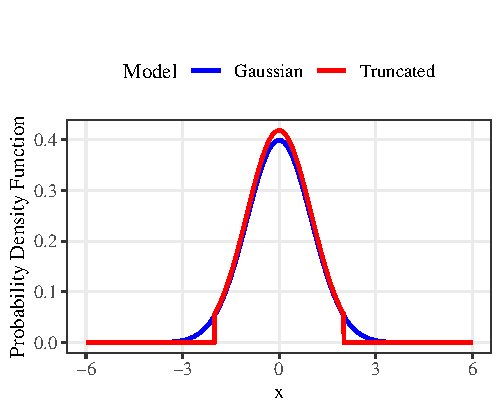
\includegraphics[width=.5\linewidth]{gaussian_vs_truncated_gaussian}}
%	\subfloat[\centering Gaussian Model Vs. Truncated Gaussian Model with translation\label{gaussian_transl_vs_truncated_gaussian_transl}]{
%		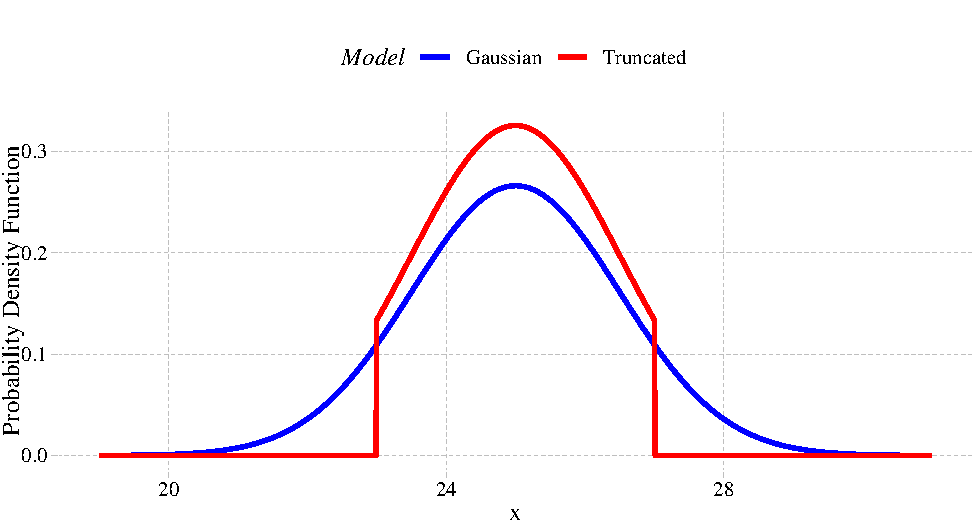
\includegraphics[width=.5\linewidth]{gaussian_transl_vs_truncated_gaussian_transl}}
%	
%	\subfloat[\centering Cauchy Model Vs. Truncated Cauchy Model\label{cauchy_vs_truncated_cauchy}]{
%		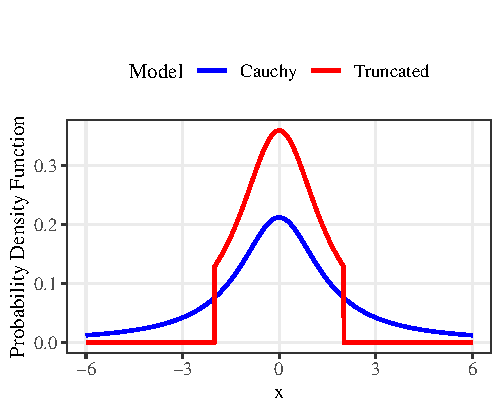
\includegraphics[width=.5\linewidth]{cauchy_vs_truncated_cauchy}}
%	\subfloat[\centering Cauchy Model Vs. Truncated Cauchy Model with translation\label{cauchy_transl_vs_truncated_cauchy}]{
%		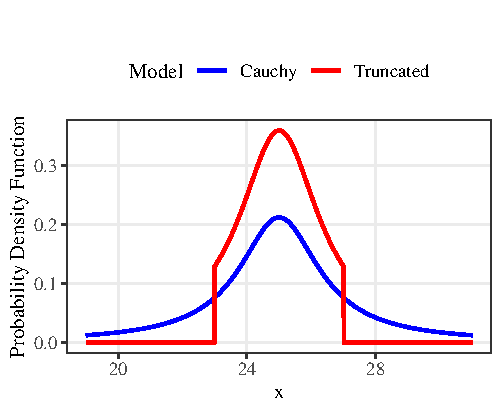
\includegraphics[width=.5\linewidth]{cauchy_transl_vs_truncated_cauchy}}
%	\caption{Equation~\eqref{eq1:_density} apply to Gaussian and Cauchy model}
%	\label{graph_gaussian_cauchy_trunc_zscore} 
%\end{figure}
%%
%% AAB - Inserir a equação da distância de KL e definir suas variáveis.
%%
%%%% JEA Equação inserida

We measure the difference between the probability density functions~\eqref{subsec:sec3.2.1_cap3Eq7} and~\eqref{subsec:sec3.2.1_cap3Eq8} with the Kullback-Leibler distance~\cite{AnalyticExpressionsforStochasticDistancesBetweenRelaxedComplexWishartDistributions}:
\begin{equation}\label{dKL}
	d_{\mathrm{KL}}(f_{X}, f_{Y}) 
	=\frac{1}{2} \int\big(f_{X}(x)-f_{Y}(y)\big) \log\left( \frac{f_{X}(x)}{f_{Y}(x)}\right) dx.
\end{equation}
With this, we quantify their discrepancy when the former uses a non-integer number of looks and the latter its closest integer. 

%We used the Kullback-Leibler distance ($d_{\text{KL}}$) to assess the discrepancy between models~\eqref{subsec:sec3.2.1_cap3Eq7} and~\eqref{subsec:sec3.2.1_cap3Eq8}. This comparison quantifies the difference between~\eqref{subsec:sec3.2.1_cap3Eq7} and~\eqref{subsec:sec3.2.1_cap3Eq8} when the former uses a non-integer number of looks and the latter its closest integer.

Table~\ref{TabDistancia} shows the Kullback-Leibler divergence between models~\eqref{subsec:sec3.2.1_cap3Eq7} and~\eqref{subsec:sec3.2.1_cap3Eq8}. We can see that as the number of looks increases, the Kullback-Leibler divergence decreases, indicating convergence. 
However, the last line of Table~\ref{TabDistancia} highlights an important point noted by Haynes~\cite{FastandAccurateComputationoftheMultilookInterferometricPhaseProbabilityDensityFunction}:
an error occurs when integrating~\eqref{subsec:sec3.2.1_cap3Eq7} for a number of looks greater than $171$.
Thus, it is not possible to calculate the distance between the expressions.
% AAB - Todas a dicas abaixo eu pensei ainda em 2025. Acredito que para o deadline ded 28/02 ficará impraticavel. (22/02/2026).
% AAB -  Por que nesse artigo está somente a distância KL entre os modelos físicos. Eu penso que pode ser apresentados todoas as distancias entre modelos. Temos espaço agora.
%
% AAB - O artigo do Hyanes indica o motivo do problema acontecer?
%
%
% AAB -  Por que nesse artigo está somente a distância KL entre os modelos físicos. Eu penso que pode ser apresentados todas as distancias entre modelos. Temos espaço agora.
%
%%%JEA Sim. De acordo com Haynes, embora analiticamente sólida, o cálculo direto da densidade multilook é esgotado para $N>170$ e $\gamma>0.9$ porque envolve produtos de fatoriais muito grandes e números muito pequenos elevados a potências altas, que levam à perda de precisão numérica em aritmética de dupla precisão. DOI: 10.1109/LGRS.2017.2679703
%
% AAB - No paragráfo acima você cita o artigo de Hyanes, mas não explica o motivo do problema. Por mais que já foi comentado no texto, quando você cita o artigo é bom comentar o problema rapidamente.
%
\begin{table}[hbt]
	\caption{Distance between physical models truncating the number of looks for $|\rho_c|=0.7$ and $\theta=0$.\label{TabDistancia}}
	\begin{tabularx}{\textwidth}{
			>{\centering\arraybackslash}X % Eq 1
			>{\centering\arraybackslash}X % Eq 2
			>{\centering\arraybackslash}X % KL distance
		}
		\toprule
		\multicolumn{2}{c}{\textbf{Looks $L$}} & \multicolumn{1}{c}{\textbf{Kullback-Leibler Distance}} \\
		\midrule
		Eq.~\eqref{subsec:sec3.2.1_cap3Eq8} & Eq.~\eqref{subsec:sec3.2.1_cap3Eq7} & $d_{\text{KL}}$ \\
		\midrule
		$3$   & $3.49$   & $\num{0.0054}$ \\
		$10$  & $10.49$  & $\num{0.0006}$ \\
		$20$  & $20.49$  & $\num{0.0002}$ \\
		$50$  & $50.49$  & $\num{2.4e-05}$ \\
		$100$ & $100.49$ & $\num{5.8e-06}$ \\
		$170$ & $170.49$ & $\num{2.1e-06}$ \\
		\midrule
		\multicolumn{3}{c}{For $L > 171$, an error occurs in model~\eqref{subsec:sec3.2.1_cap3Eq7}.} \\
		\bottomrule
	\end{tabularx}
\end{table}
%
% AAB - Aqui tem que fazer outra tabelas com os resultados das distância entre as truncadas também, por que somente os resultados entre as fisicas? 
%

%Based on the data presented in Table~\ref{TabDistancia}, the distance $d_{\text{KL}}$ between the models defined in~\eqref{subsec:sec3.2.1_cap3Eq7} and~\eqref{subsec:sec3.2.1_cap3Eq8} reveals important aspects, as described below. 
%As the number of looks increases, $d_{\text{KL}}$ gradually decreases, indicating greater similarity between the models. 
%Figure~\ref{ajuste_dKL_fisicos} illustrates those differences.
%For instance, for $L = 3$, $d_{\text{KL}}$ is $0.0054$, whereas for $L = 170$, it is $\num{2.1e-06}$, suggesting that for high values of $L$, the expressions tend to converge. 
%The data presented in Table~\ref{TabDistancia} and illustrated in Figure~\ref{ajuste_dKL_fisicos} show the relationship between $d_{\text{KL}}$ and the number of looks, indicating that as $L$ increases, the models become increasingly similar. 
%In the Figure, the model~\eqref{subsec:sec3.2.1_cap3Eq7} is represented in blue, while the model in~\eqref{subsec:sec3.2.1_cap3Eq8} is represented in red.  
%
% AAB - Ajustar os gráficos as margens do trabalho. Feito!!!!
%
%
% AAB - Mesma obs anterior. 22/02/2026
% AAB - Reorganizar os gráficos inserindo grafico com as distância entre as truncadas. Além disso refletir se os gráficos com L >50 valem a pena estar no artigo, pois os gráficos estão um em cima do outro, não dá para ver diferênça. Mas se quisermos deixar os gráficos não vejo problema. 
%
%\begin{figure}[hbt]
%	%\begin{adjustwidth}{-\extralength}{0cm}
%	%\begin{adjustwidth}
%	\centering
%	\subfloat[\centering\parbox{\linewidth}{Blue $L=3.49$, red $L=3$}\label{p1}]{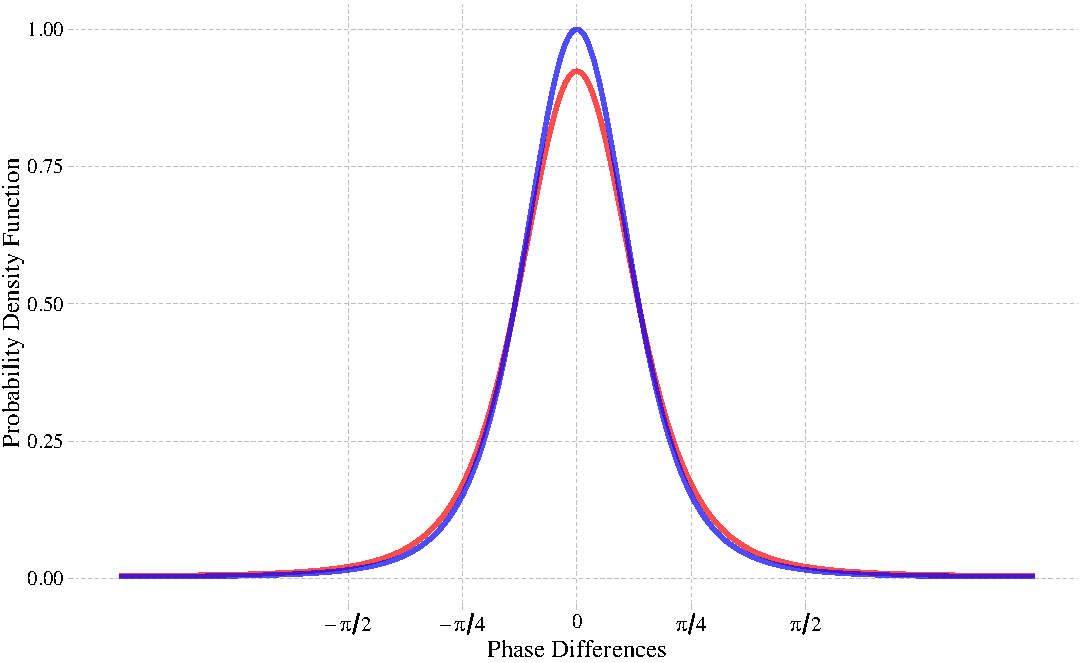
\includegraphics[width=.45\linewidth]{Lee3.49_Gierull3}}
%	\subfloat[\centering\parbox{\linewidth}{Blue $L=10.49$, red $L=10$}\label{p2}]{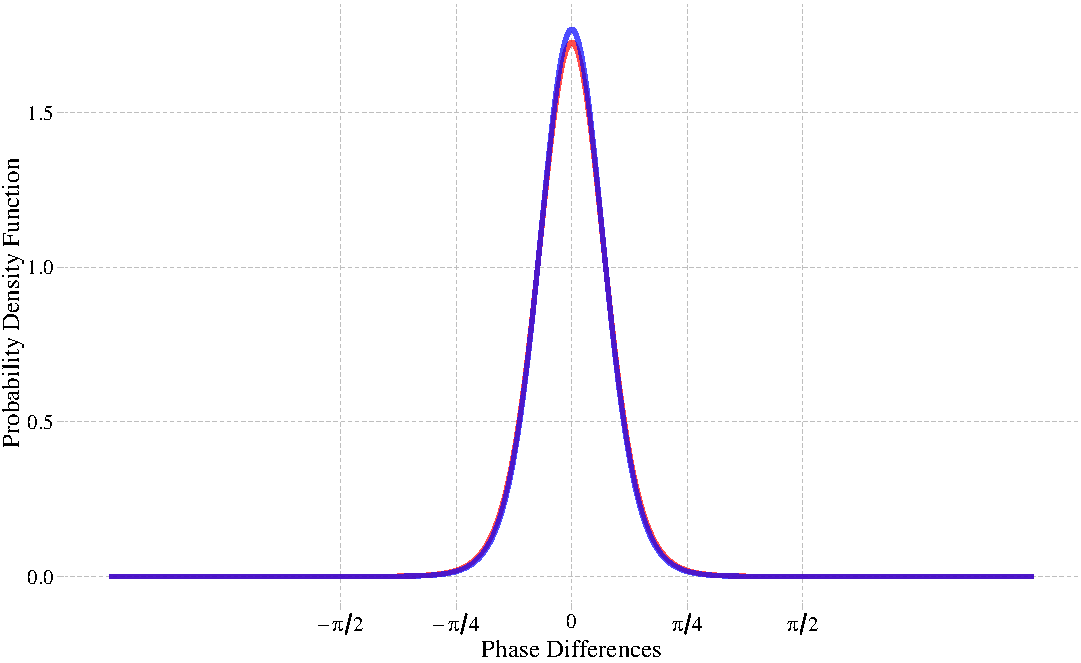
\includegraphics[width=.45\linewidth]{Lee10.49_Gierull10}}
%	
%	\subfloat[\centering\parbox{\linewidth}{Blue $L=20.49$, red $L=20$}\label{p3}]{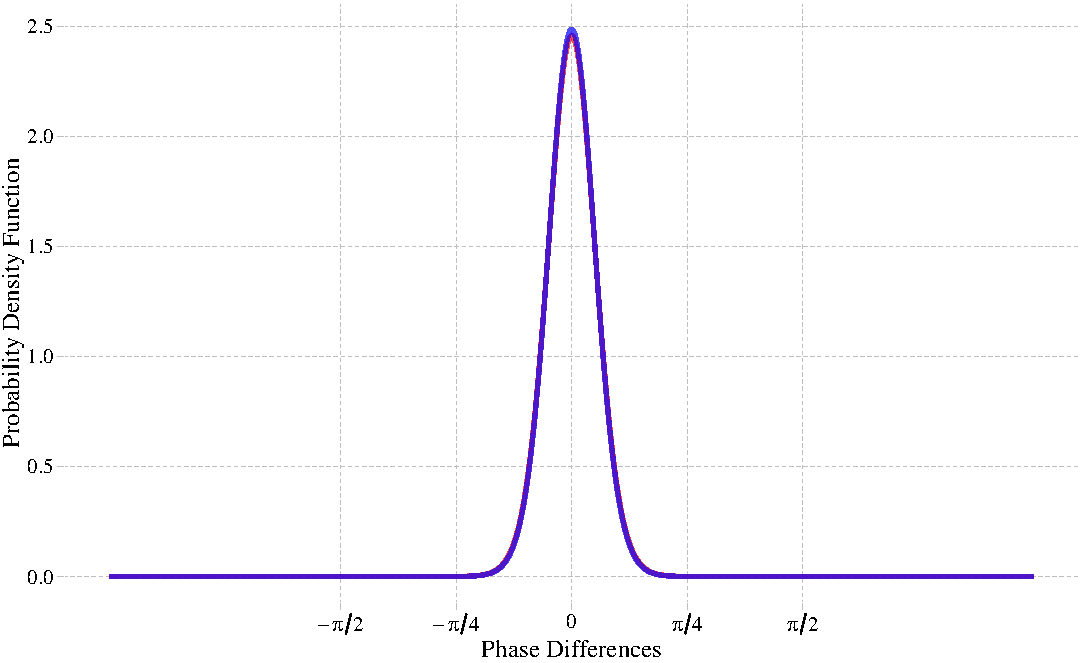
\includegraphics[width=.45\linewidth]{Lee20.49_Gierull20}}
%	\subfloat[\centering\parbox{\linewidth}{Blue $L=50.49$, red $L=50$}\label{p4}]{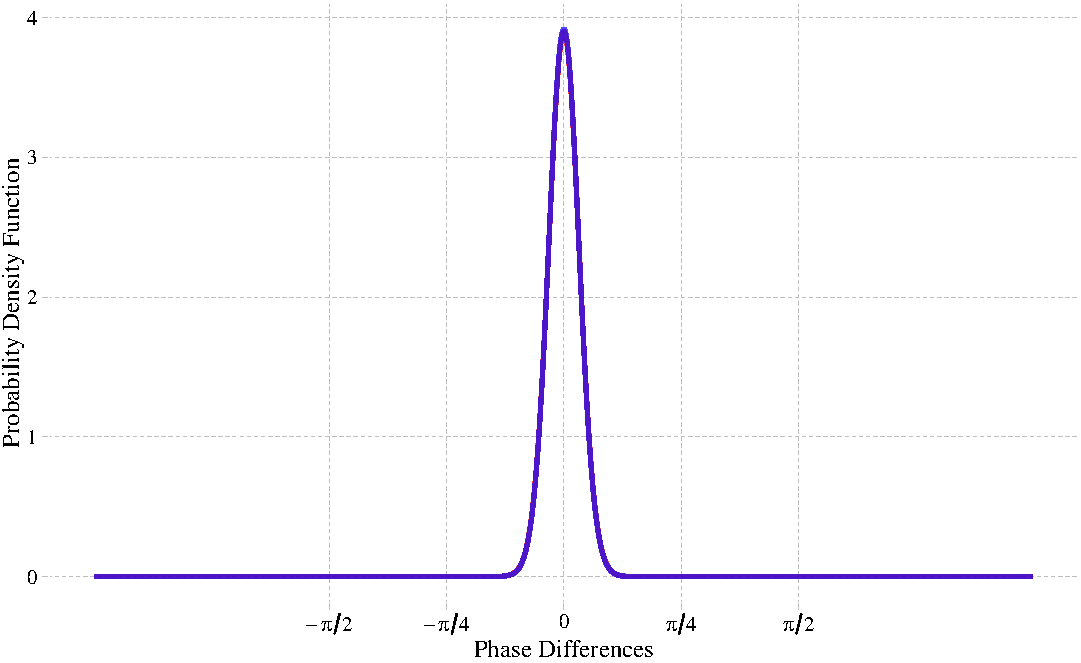
\includegraphics[width=.45\linewidth]{Lee50.49_Gierull50}}
%	
%	\subfloat[\centering\parbox{\linewidth}{Blue $L=100.49$, red $L=100$}\label{p5}]{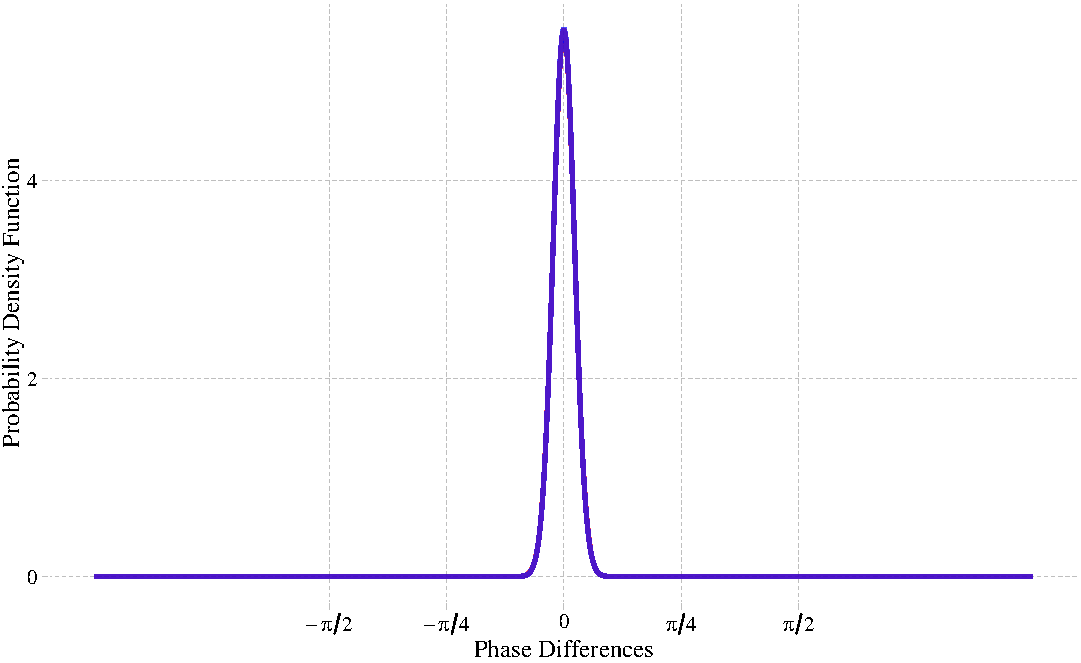
\includegraphics[width=.45\linewidth]{Lee100.49_Gierull100}}
%	\subfloat[\centering\parbox{\linewidth}{Blue $L=170.49$, red $L=170$}\label{p6}]{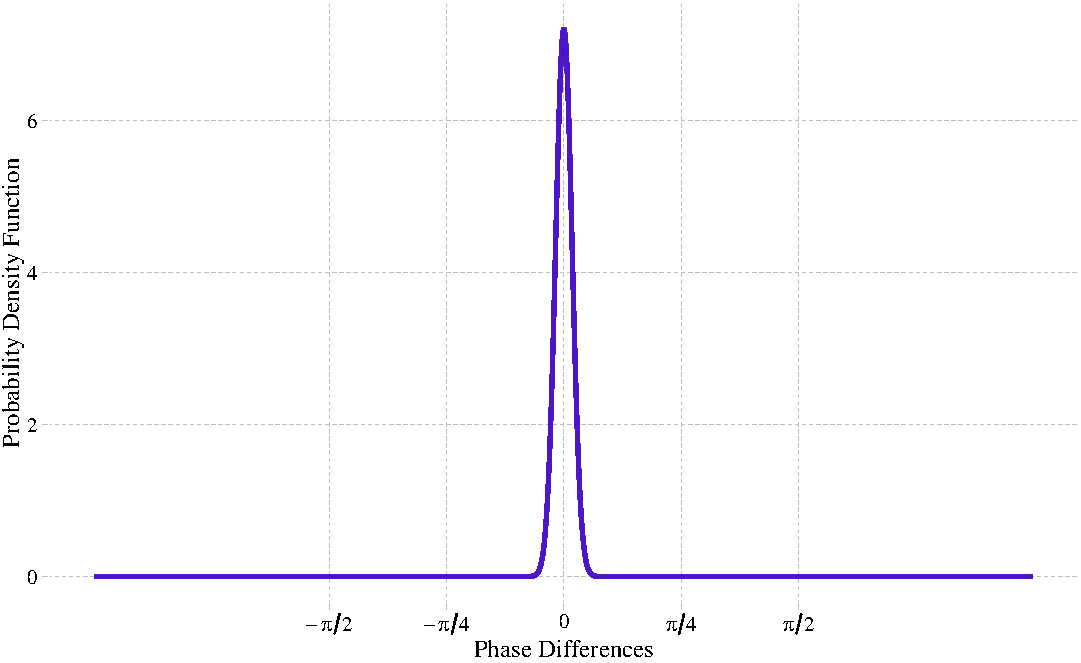
\includegraphics[width=.45\linewidth]{Lee170.49_Gierull170}}
%	%\end{adjustwidth}
%	\caption{\textmd{Similarity between the physical models in relation to the Kullback-Leibler divergence}}
%	\label{ajuste_dKL_fisicos} % label da figura toda
%\end{figure}

%In the Figures~\ref{p3}, \ref{p4}, \ref{p5} and~\ref{p6}, we can see a strong similarity between the models; in these cases, the lines overlap. With the goal of better understanding the behavior, we designed the following graphics. 
Figure~\ref{erro_modelos} shows the pointwise absolute errors between the expression in~\eqref{subsec:sec3.2.1_cap3Eq7}, indexed by $L = 3.49, 5.49, 7.49, 9.49$, and the expression in~\eqref{subsec:sec3.2.1_cap3Eq8}, fixing $L = 3, 5, 7, 9$. 

\begin{figure}[hbt]
\centering
	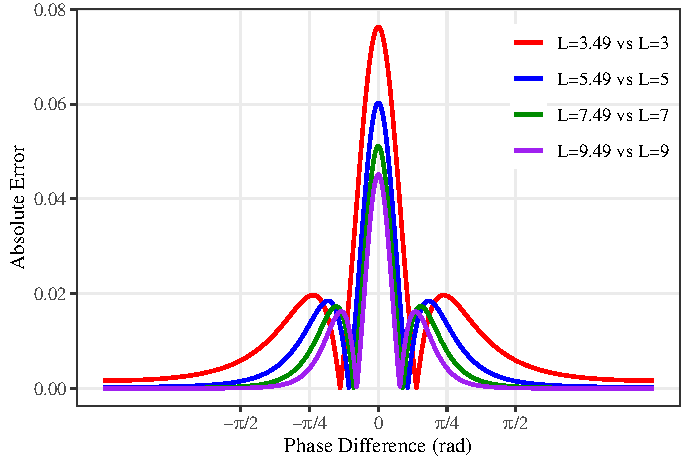
\includegraphics[width=.7\linewidth]{absolute_error}
	\caption{\textmd{Absolute error between~\eqref{subsec:sec3.2.1_cap3Eq7} and~\eqref{subsec:sec3.2.1_cap3Eq8}: $L=3.49$ vs.\ $L=3$ (red), $L=5.49$ vs.\ $L=5$ (blue), $L=7.49$ vs.~$L=7$ (green), and $L=9.49$ vs.\ $L=9$ (purple)}}
	\label{erro_modelos} % label da figura toda
\end{figure}

The largest error occurs when $L = 3$ for the model in~\eqref{subsec:sec3.2.1_cap3Eq8} and $L = 3.49$ for the model in~\eqref{subsec:sec3.2.1_cap3Eq7} (red), while the smallest error is observed when $L = 9$ for the model in~\eqref{subsec:sec3.2.1_cap3Eq8} and $L = 9.49$ for the model in~\eqref{subsec:sec3.2.1_cap3Eq7} (purple). Therefore, the error decreases with $L$ and is concentrated on the bulk of the PDF, i.e., it affects the tails less.

The decrease in error as the value of $L$ increases suggests that, for integer values of $L$ greater than 1, the use of the model in~\eqref{subsec:sec3.2.1_cap3Eq8} does not result in a significant loss of accuracy compared to the model in~\eqref{subsec:sec3.2.1_cap3Eq7}. 
As the number of looks increases, the accuracy of the model in~\eqref{subsec:sec3.2.1_cap3Eq8} improves, resulting in smaller absolute differences between the models.

%In the Figures~\ref {p3}, \ref{p4}, \ref{p5} and~\ref{p6} we can see a great similarity between the models; in these cases, the lines in the graphics are overcome. With the goal of better understanding the behavior, we designed the following graphics. Therefore, Figure~\ref{erro_modelos} shows the pointwise absolute errors between the expression in~\eqref{subsec:sec3.2.1_cap3Eq7}, indexed by $L = 3.49; 5.49; 7.49; 9.49$, and the expression in~\eqref{subsec:sec3.2.1_cap3Eq8}, assuming $L = 3; 5; 7; 9$. As observed in Figure~\ref{erro_modelos}, the decrease in error as the value of $L$ increases suggests that, for integer values of $L$ greater than 1, the use of the model in~\eqref{subsec:sec3.2.1_cap3Eq8} does not result in a significant loss of accuracy compared to the model in~\eqref{subsec:sec3.2.1_cap3Eq7}. As the number of looks increases, the accuracy of the model in~\eqref{subsec:sec3.2.1_cap3Eq8} approaches or converges to that of the model in~\eqref{subsec:sec3.2.1_cap3Eq7}, resulting in smaller absolute differences between the models.

%The absolute error reflects the numerical discrepancy between the predicted results and the actual values. 
%According to Figure~\ref{erro_modelos}, 


% AAB - Acho que devemos inserir todas as proposições de filtro como metodologia, já fiz a troca.
% AAB - Eu inseri a subseção sobre a estimativa do $\rho$

Figure~\ref{fig:std_dev_vs_coherence_Gierull} shows 
the standard deviation
of a random variable that follows the Gierull interferometric phase model as a function of coherence $\rho_c$ and the number of looks $L$,
obtained by numerical integration using the Gauss-Kronrod quadrature algorithm~\cite{Orive2022}.
The variability of such random variable decreases when the number of looks increases, and depends on the value of the coherence.

\begin{figure}[hbt]
	\centering
	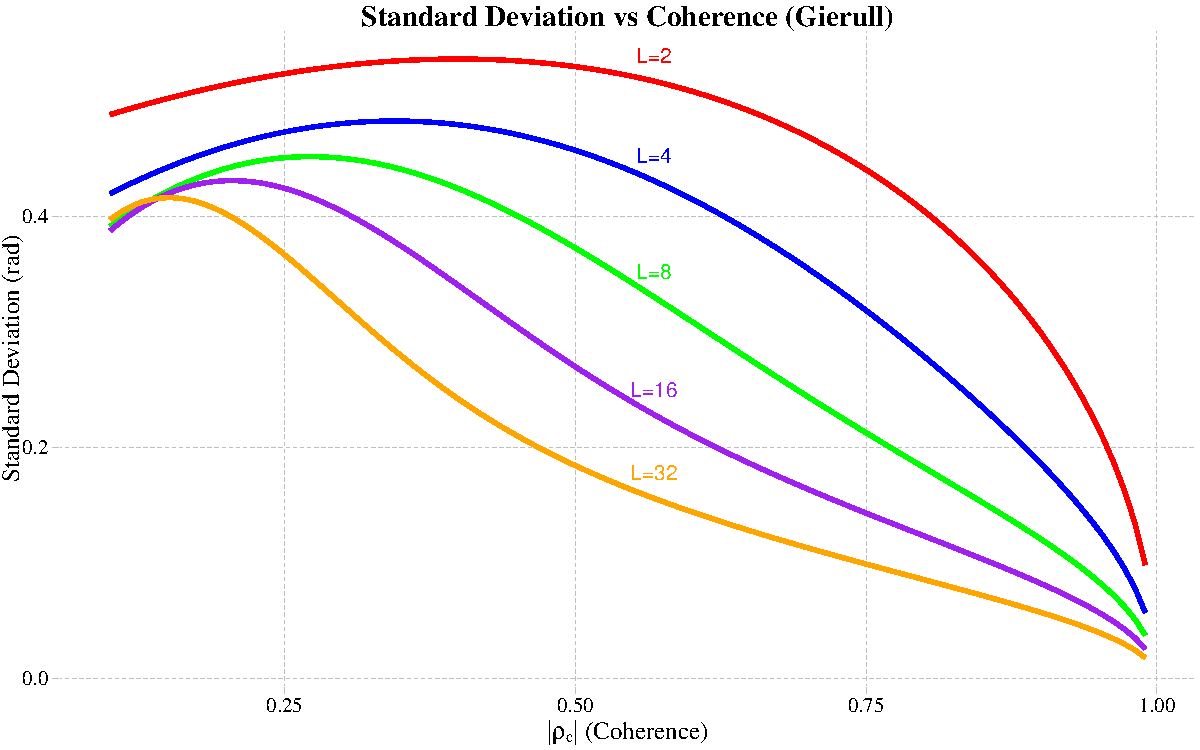
\includegraphics[width=.7\linewidth]{std_dev_vs_coherence_Gierull}
	\caption{Numerical approximation of the standard deviation of the interferometric phase noise as a function of coherence $\rho_c$ and the number of looks L.}
	\label{fig:std_dev_vs_coherence_Gierull} % label da figura toda
\end{figure}


\subsubsection{Coherence Estimation and Unwrapping}\label{subsec:Coherence_est}

%We can consider the speckle in the SAR intensity image as a phase-noise characteristic generated by the coherent interference of waves reflected from many elementary scatterers. Noise in InSAR images can be considered the interaction of two correlated processes: a coherent interference process. 

Coherence estimation is essential in filtering techniques. 
%In this subsection, we summarize how to estimate coherence and choose not to include the time required for the coherence estimator in each filter processing time in the results section.
The Maximum Likelihood Estimator (MLE) based on~\eqref{subsec:sec3.2.1_cap3Eq8} 
for the random sample  
$\bm{\psi} = (\psi_1, \psi_2, \dots, \psi_n)$ maximizes the log-likelihood function:
\begin{multline}
\mathcal{L}(\rho_c; \bm{\psi}, \theta, L) = \ln \prod_{i=1}^{n} f(\psi_i; \theta, \rho_c, L) = \sum_{i=1}^{n} \ln f(\psi_i; \theta, \rho_c, L) = \\ 
\sum_{i=1}^{n}\ln\Bigg(\frac{(1-\rho_c^2)^L}{2\pi\Gamma(L)(1-\beta_i^2)^{L+\frac{1}{2}}}\left\lbrace \sqrt{\pi}\Gamma\Big(L+\frac{1}{2}\Big)\beta_i\right.\\
	+\frac{\Gamma\big(L-\frac{1}{2}\big) }{\sqrt{\pi}}\bigg[ \sqrt{1-\beta_i^2}+2\Big(L-\frac{1}{2}\Big)\beta_i\arcsin\beta_i\bigg]\\ 
	\mbox{}+\sum_{k=1}^{L-1}\frac{(-1)^k}{2}\frac{\Gamma\big( k-L+\frac{1}{2}\big) \Gamma(L-k)}{\Gamma\big( \frac{3}{2}-L\big) }
	\left.\frac{1+(2k-1)\beta_i^2}{(1-\beta_i^2)^{k-L+\frac{1}{2}}}\right\rbrace\Bigg),
\label{eq:LogLikelihood}
\end{multline}
where, $\beta_i=|\rho_c|\cos(\psi_i-\theta)$.
The parameters $\theta$ and $L$ are considered constant. 
We estimate the coherence locally 
with sliding windows of size 
$3 \times 3$. 

%The Figure~\ref{fig:coherence_insar} shows the original InSAR image (right) and map of estimated coherence values (left).
%
%\begin{figure}[hbt]
%	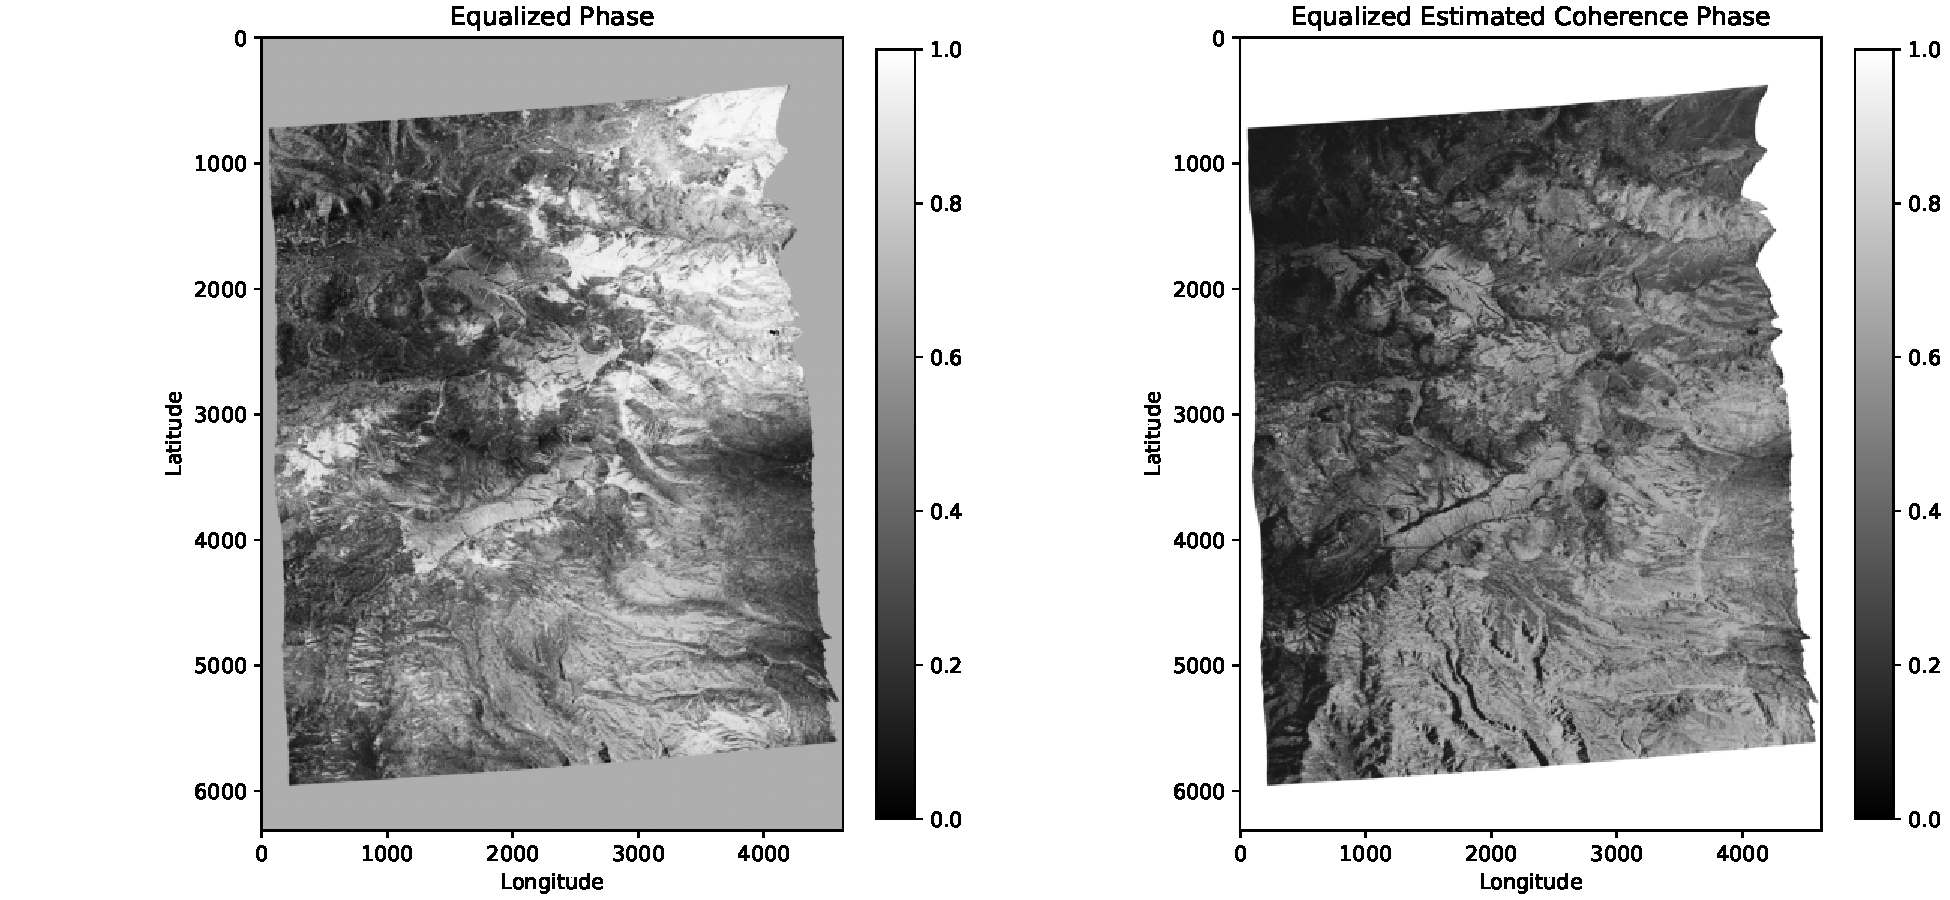
\includegraphics[width=\textwidth]{los_alamos_orig_and_coherence.pdf}
%	\caption{\textmd{Left: Los Alamos InSAR Image. Right: estimated coherence InSAR map.}}
%	\label{fig:coherence_insar}
%\end{figure}
%
%We present only the Los Alamos image as an example, as the procedure for the remaining images is identical.
%These images interfere with the results presented in this article and have been included in the text for informational purposes.
%
%\subsubsection{Phase Unwrap InSAR technics}\label{subsec:phase_unwrap}

We used the technique 
discussed by \citet{DomnguezGuzmn2009}
to unwrap the phase. 
In the sequel, we show equalized images to facilitate their visualisation.
 
%\begin{figure}[hbt]
%	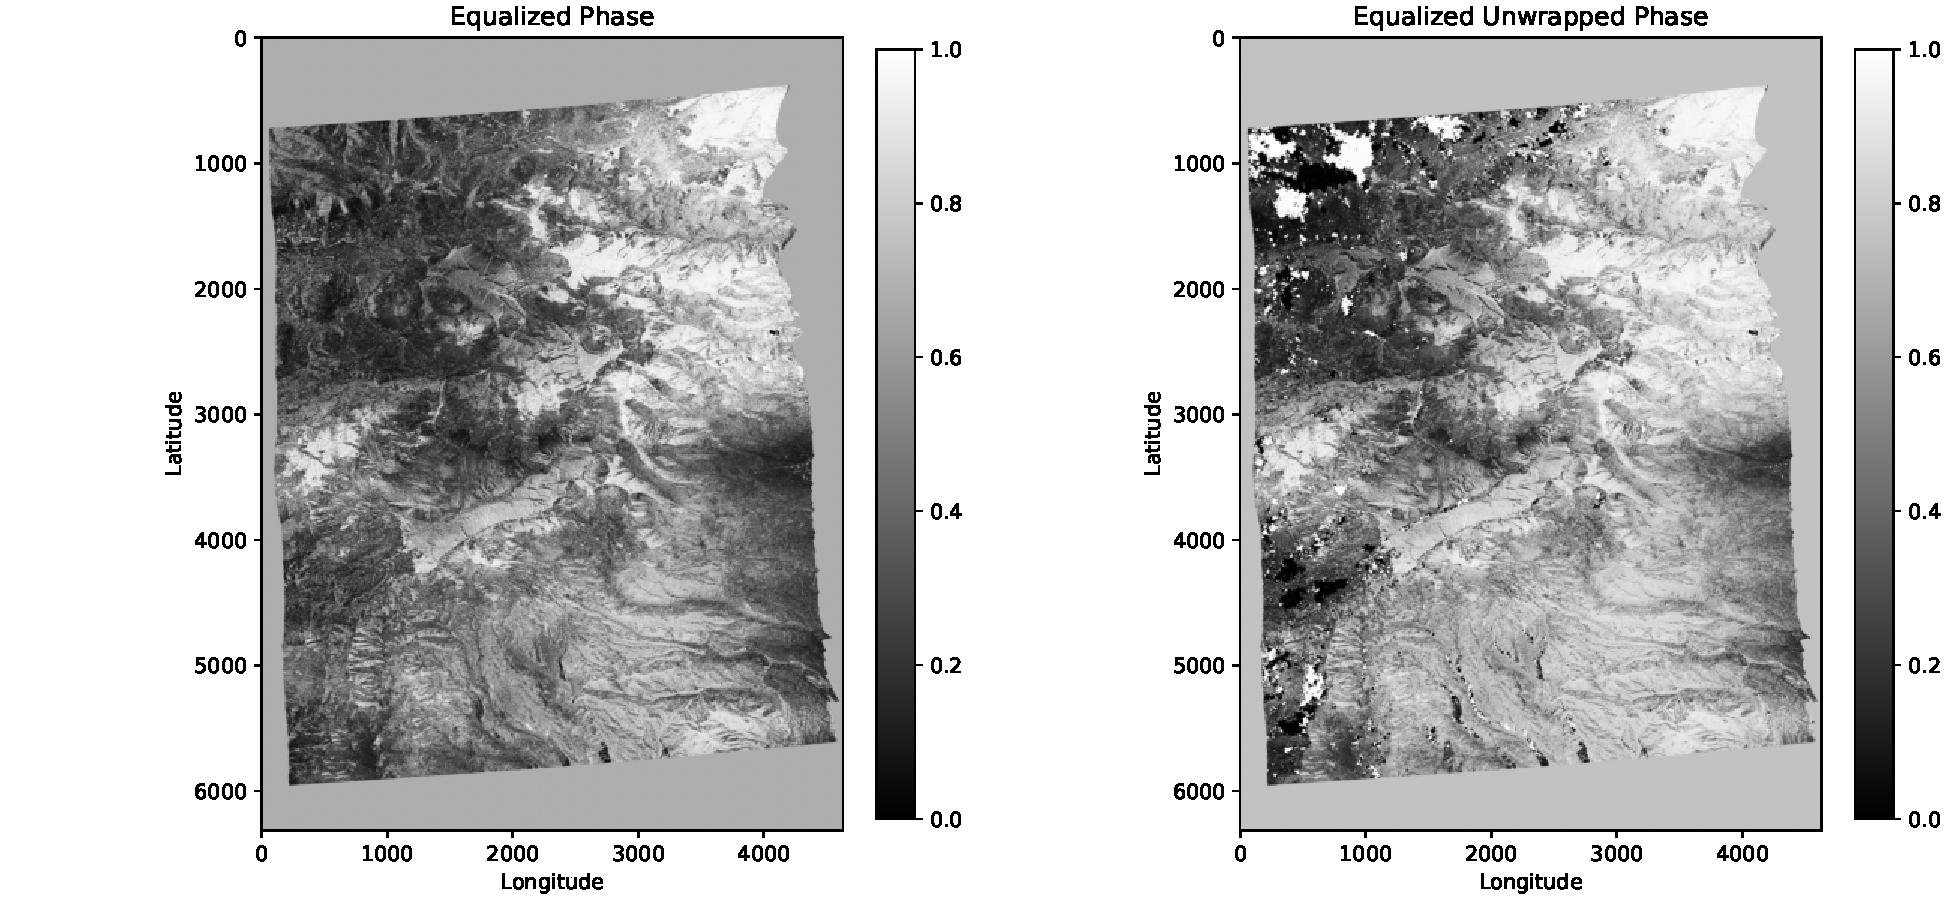
\includegraphics[width=\textwidth]{los_alamos_orig_and_wrapped.pdf}
%	\caption{\textmd{Left: Los Alamos InSAR Image, Right: Los Alamos Unwrapped InSAR image}}
%	\label{fig:unwrap_insar}
%\end{figure}

% Imagem com a phase original e a phase desembrulhada proveniente do repositório UAVSAR
%\begin{figure}[hbt]
%	\subfloat[\centering InSAR regular phase in 2D\label{fig:unwrap_insar_a}]{
%		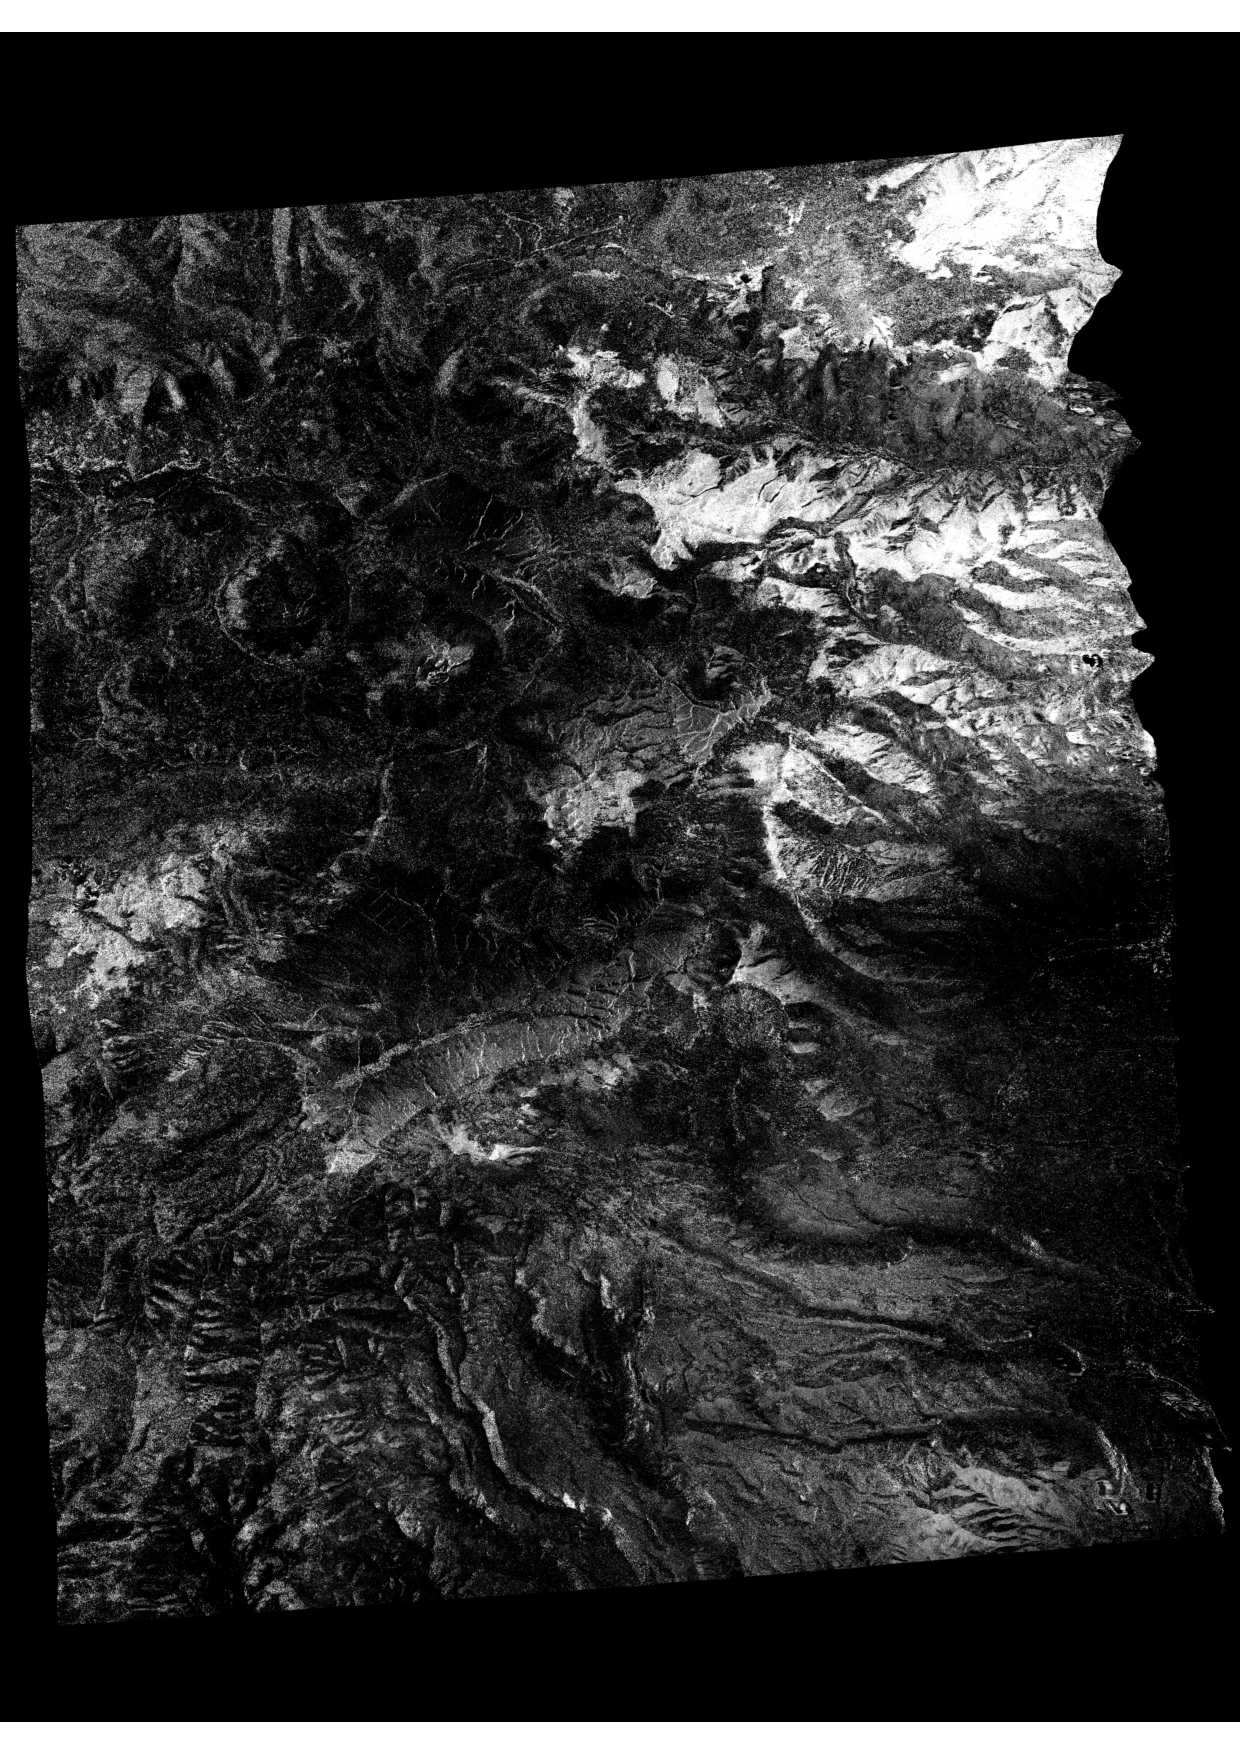
\includegraphics[width=0.5\textwidth]{alamos_35915_20008-000_20013-000_0007d_s01_L090HH_02_PHS_raw.pdf}}
%	\subfloat[\centering InSAR wraped phase in 2D\label{fig:unwrap_insar_b}]{
%		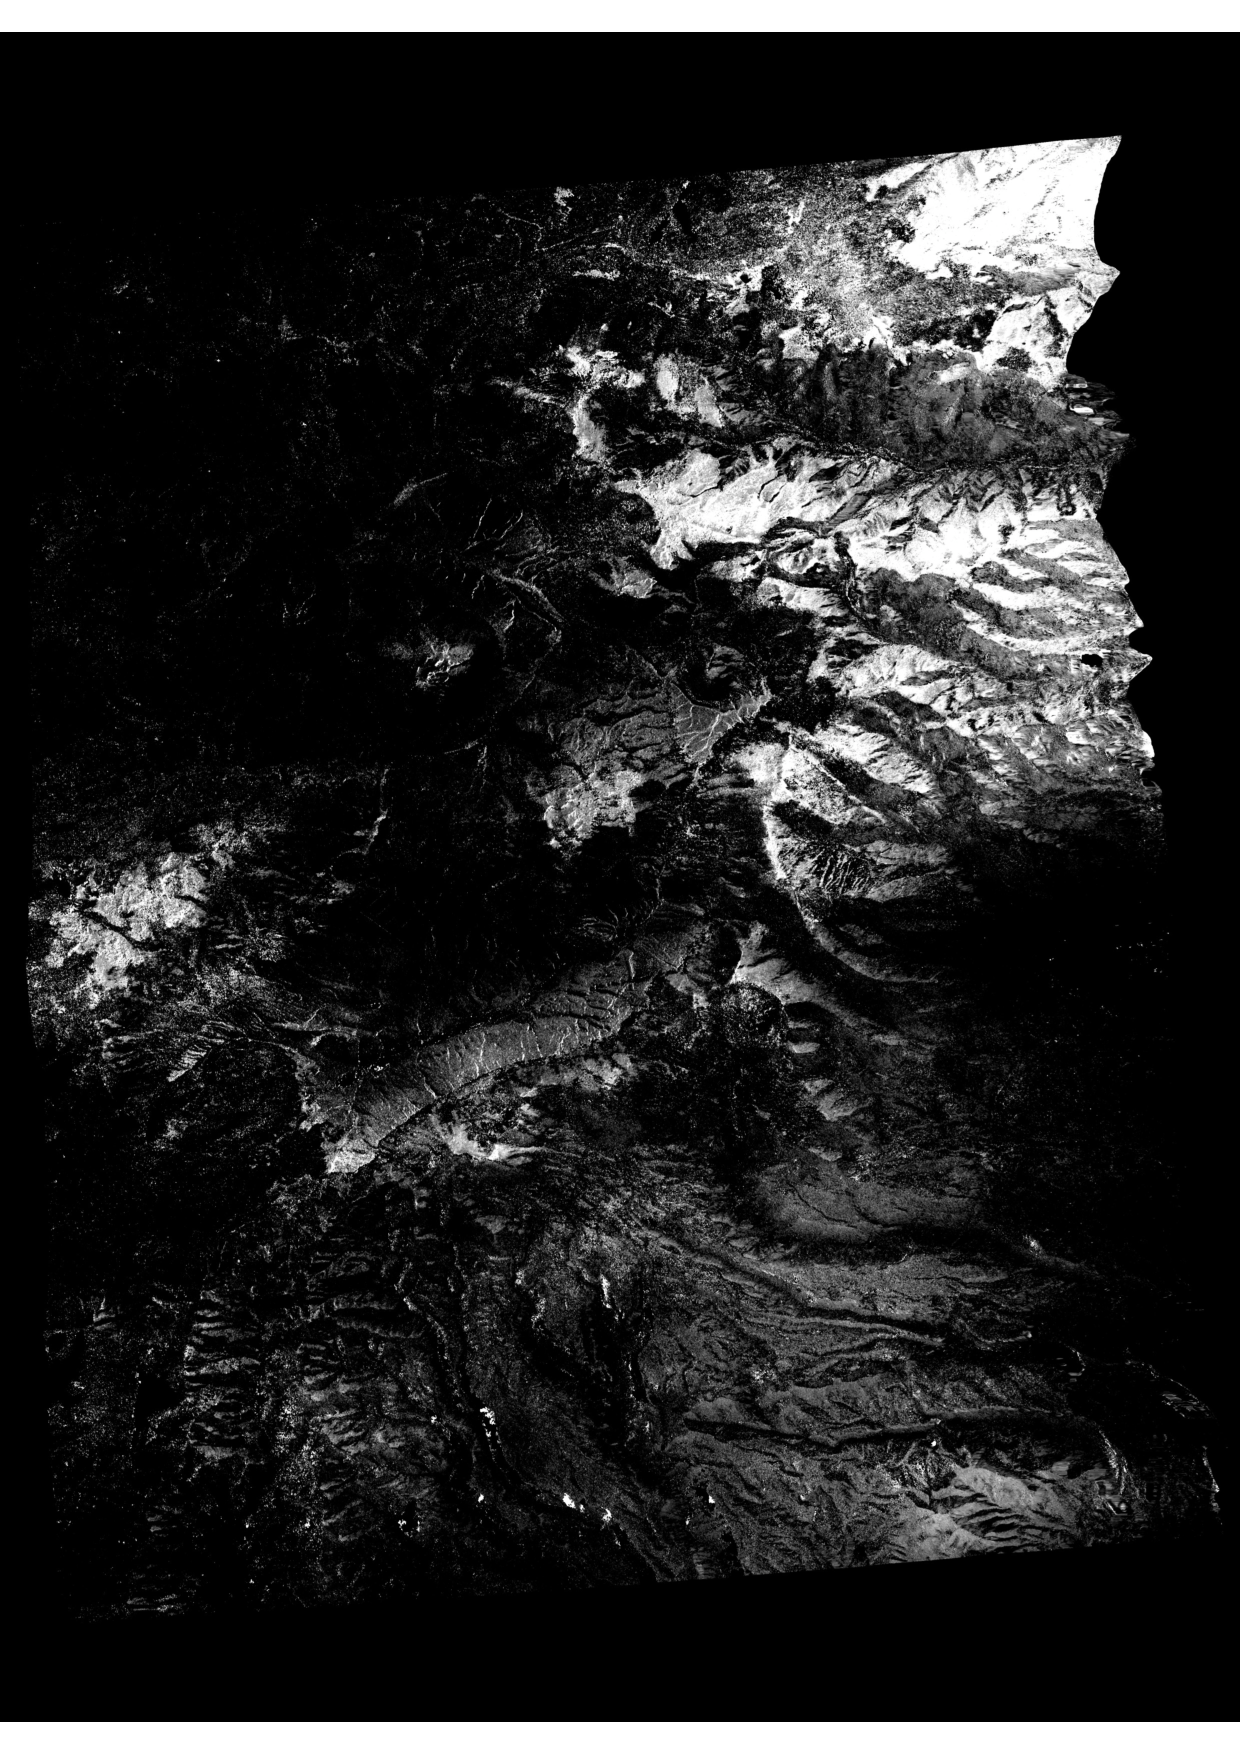
\includegraphics[width=0.5\textwidth]{alamos_35915_20008-000_20013-000_0007d_s01_L090HH_02_UNW_raw.pdf}}\\
%	\caption{\textmd{UAVSAR regular and wraped phase in 2D and 3D}}
%	\label{fig:unwrap_insar}
%\end{figure}
%
\subsubsection{Lee InSAR Adaptive Filter}\label{sec:lee_filter}

Several algorithms for filtering InSAR phase noise have been proposed in the past. 
As previously mentioned, a group of filters includes spatial-domain filters such as Boxcar, median, and mean. 
All of them are effective at reducing noise in homogeneous, flat areas, but they generally fail to preserve fringe patterns in steep regions. 
Recognizing the difficulty of reducing phase noise in sloped areas, \citet{AnewtechniquefornoisefilteringofSARinterferometricphasimages} proposed an adaptive algorithm that does not use a conventional square window, but instead selects one out of $16$ directional windows (see Figure~\ref{Janelas_filtroInSAR_Lee}) seeking alignment with the fringes of the InSAR image.

\begin{figure}[hbt]
\centering
	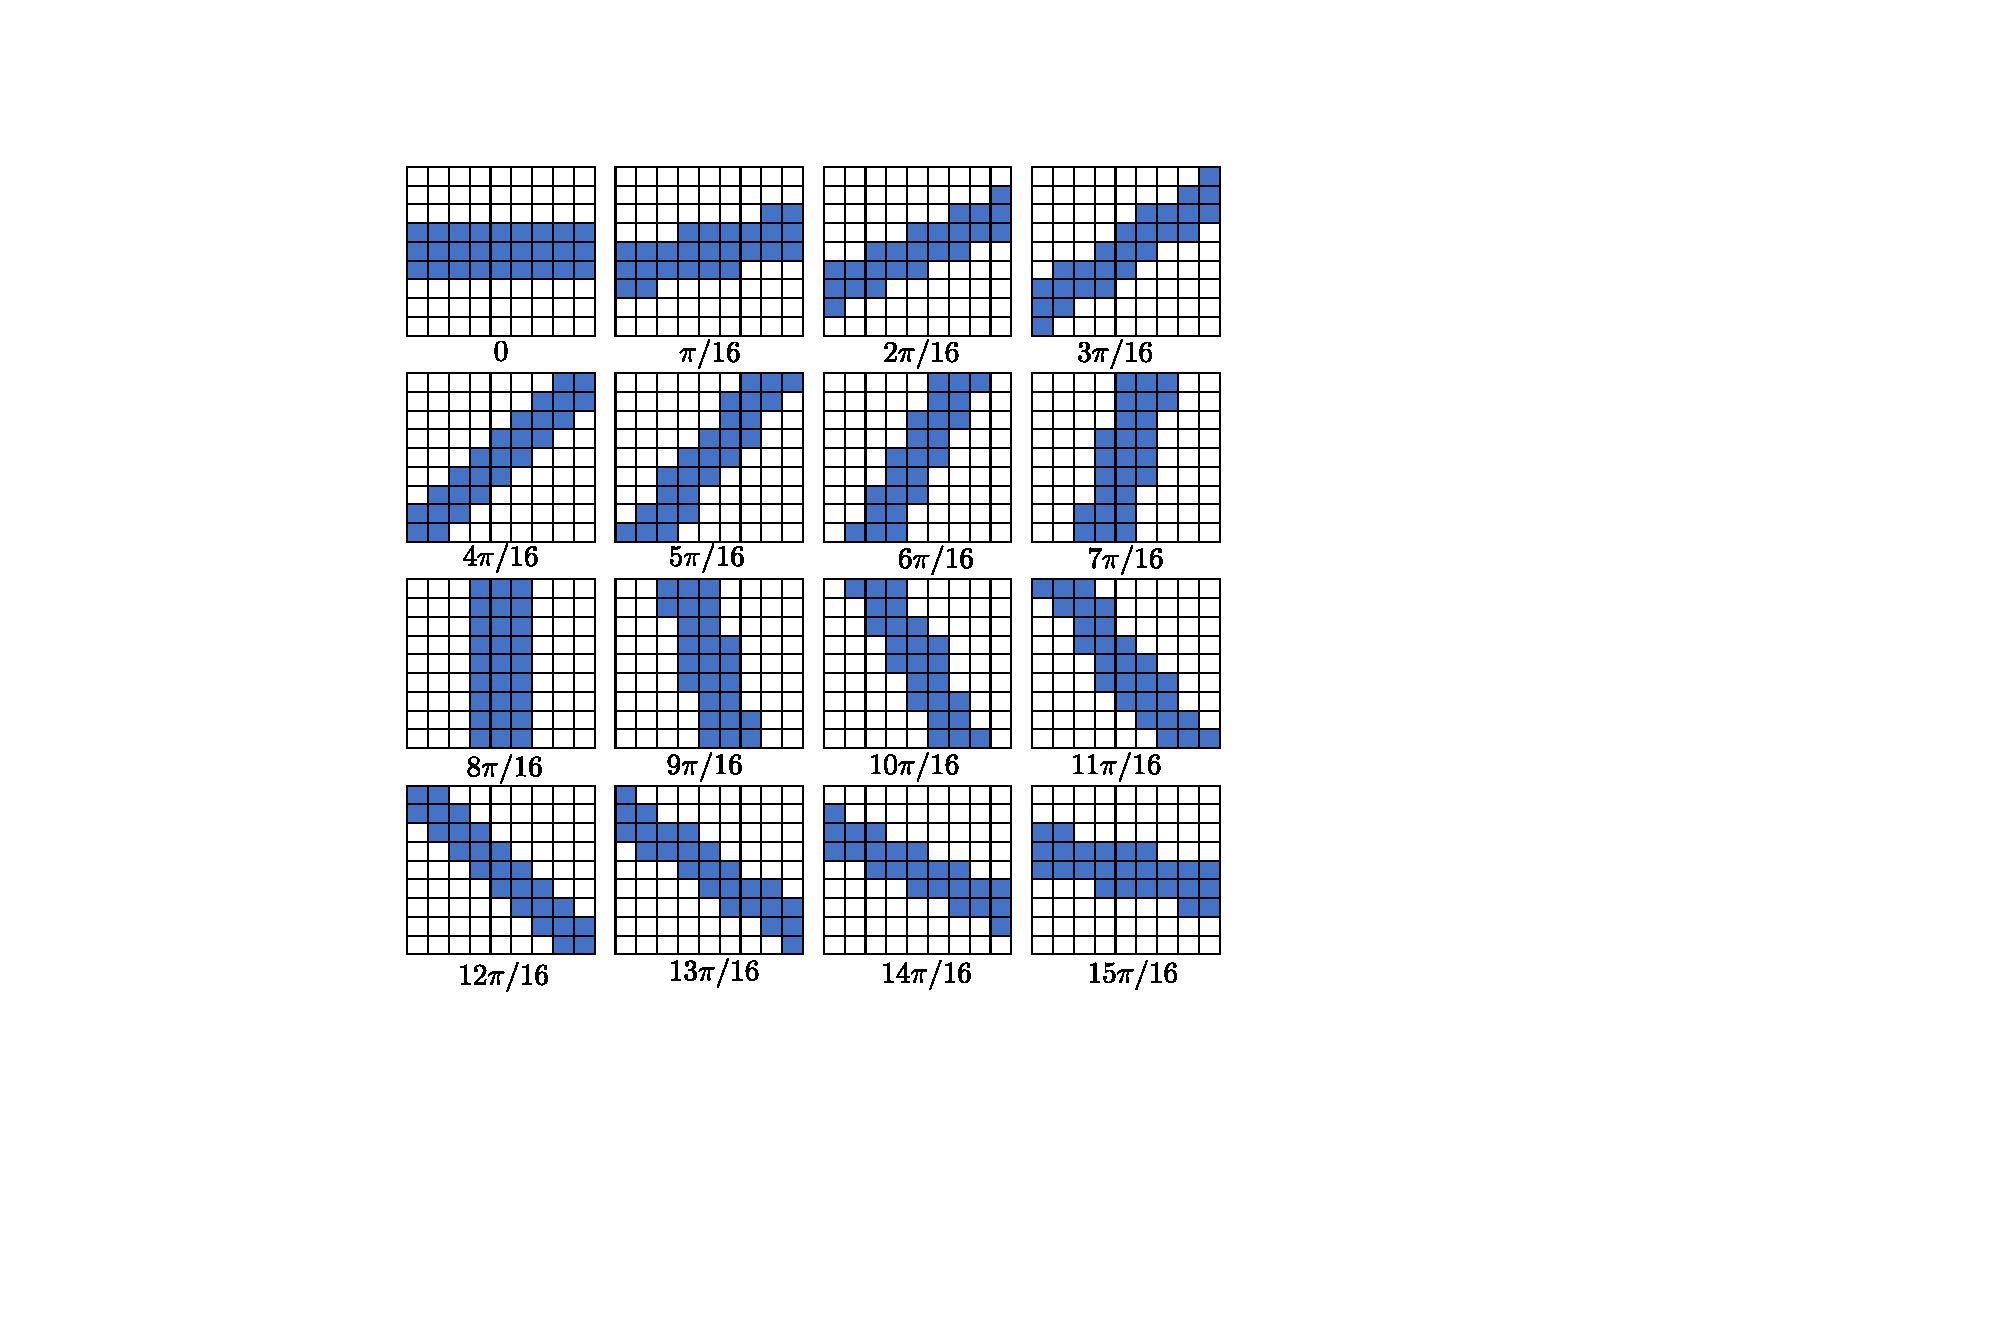
\includegraphics[width=0.7\textwidth]{Janelas_filtroInSAR_Lee}
	\caption{\textmd{Sixteen directional $9\times 9$ masks for phase noise filtering}}
	\label{Janelas_filtroInSAR_Lee}
\end{figure}

The Lee InSAR filter uses an additive noise model, assuming that the noise standard deviation depends on the number of looks and coherence; however, the filter depends on the local variance and the estimated coherence. 
To this end, it computes the local mean and adaptively applies a Minimum Mean Square Error (MMSE) filter. 
The Lee InSAR filter was specifically designed to adjust to the direction of the fringes.

Subsequently, \citet{RefinedFilteringofInterferometricPhaseFromInSARData} refined this method by introducing a filter based on directional windows and the exclusion of unreliable pixels, using an enhanced sigma filter. 
In the Refined Lee InSAR filter, the operations are applied only to pixels whose phase lies within a symmetric interval around the phase of the central pixel, determined by a proportion $\xi$, computed from the probability density function of the phase difference. 
This approach better preserves fringe patterns and significantly reduces the number of residues after filtering.

%In this subsection, we outline the Lee filter approach. 
We replaced the Lee model~\eqref{subsec:sec3.2.1_cap3Eq7} by the Gierull representation~\eqref{subsec:sec3.2.1_cap3Eq8}, and 
maintained the other characteristics of the Refined Lee InSAR filter. 
%considered the noise as additive, that is, $\bm{\psi}_o=\bm{\psi}_r + \mathcal{N}$, where,  $\bm{\psi}_o$ is the observed phase, $\bm{\psi}_r$ is true phase, and the noise $\mathcal{N}$.  

\subsubsection{Refined Lee InSAR Filter}\label{sec:refined}

The Refined InSAR Lee filter presented by Chao et al.~\cite{RefinedFilteringofInterferometricPhaseFromInSARData} 
consists of the following steps
to process the central pixel in a $\kappa\times \kappa$ window, with $\kappa=9$.
Firstly, choose one out of $16$ directional windows (Figure~\ref{Janelas_filtroInSAR_Lee}) based on the maximum magnitude $|\langle e^{\mathrm{i}\psi_z}\rangle|$, where $\psi_z$ is the phase of each pixel in the window, and $\langle \cdot \rangle$ is the spatial average. If $|\langle e^{\mathrm{i}\psi_z}\rangle|$ is greater than the empirically defined threshold $\epsilon_{\text{th}}$, then the window angle is determined. Otherwise, the window angle needs to be revised using an $\kappa\times \kappa$ window, with $\kappa= 11$, to provide a more reliable estimation of the fringe direction using a new scheme called Inverse Distance Weighting (IDW).

The IDW method consists of interpolating the central pixel's window angle based on the neighbor angles of the pixels using:
\begin{equation}\label{subsec:sec3.7.2_cap3Eq}
	d_{pq}=\dfrac{1}{d(p,q)},
	\text{ and }
	e^{\mathrm{i}\widehat{\gamma}}= \dfrac{\sum\limits_{p, q=1}^{\kappa} d_{pq} e^{\mathrm{i}\gamma(p, q)}}{\sum\limits_{p,q=1}^{\kappa}d_{pq}},
\end{equation}
where $d(p,q)$ is the Euclidean distance from the center pixel $(m, n)$ to an arbitrary pixel $(p,q)$ in the window, and $\gamma(p, q)$ is the angle of pixel $(p, q)$ in the $\kappa \times \kappa$ window. 
Therefore, one of the $16$ windows whose angle is closest to the weighted angle $\widehat{\gamma}$ will be designated as the new window.

The steps comprising the Refined Lee InSAR filter algorithm are: 
$i$)~Improve the selection of directional windows for unreliable pixels; 
$ii$)~Select proper pixel in directional window, 
and $iii$)~Compute the MMSE estimator. 
Further details can be found in Refs.~\cite{RefinedFilteringofInterferometricPhaseFromInSARData, EnhancedInterferometricPhaseNoiseFilteringoftheRefinedInSARFilter}.

\subsubsection{Proposed Filtering Algorithms}\label{sec:pro}

The Enhanced Refined InSAR filter~\cite{EnhancedInterferometricPhaseNoiseFilteringoftheRefinedInSARFilter} is an improvement of the Refined InSAR filter proposed by \citet{RefinedFilteringofInterferometricPhaseFromInSARData}.
It consists of two steps: 
(i)~selecting a subset of spatially contiguous and homogeneous observations, 
and (ii)~computing their trimmed circular mean.
Our proposal begins at the second step; therefore, details of the sample selection step are omitted here.

Assume a sample of observed phases is selected, denoted by $\bm{\psi'} = (\psi'_1, \psi'_2, \dots, \psi'_N)$ of the observed phases. For filtering, the phases $\psi_z$ are selected within the interval $\bm\psi_z' = (\psi_c - \psi_\xi, \psi_c + \psi_\xi]$, where $\psi_\xi$ is the phase limit corresponding to the desired proportion $\xi$. The value of $\psi_\xi$ is computed numerically by solving:
\begin{equation}\label{Eq_limite_fase}
	F(\psi_\xi) - F(-\psi_\xi) = \xi,
\end{equation}
where $F$ is the cumulative distribution function (CDF) of the adopted model. 
According to \citet{RefinedFilteringofInterferometricPhaseFromInSARData}, the value of $\psi_\xi$ can be numerically obtained from $\xi$ for all pixels. 
In other words, the phase limit can be computed only once for the entire image, and the authors propose $\xi=0.9$ as the optimal value.

We present three methods for phase noise filtering: TcNfilter, TcCfilter, and LInSARRFE. 
The first two use the empirical models $\mathcal{NT}$ and $\mathcal{CT}$ to compute the phase limit, respectively. 
LInSARRFE calculates $\psi_{\xi}$ using the expression defined in~\eqref{subsec:sec3.2.1_cap3Eq8} for integer values of $L$ greater than $1$. For the proposed filters, $20$ directional $11\times11$ windows were created (Figure~\ref{Janelas_filtros_propostos}), and an algorithm was developed to select the one containing pixels with the most homogeneous phases~\cite{EnhancedInterferometricPhaseNoiseFilteringoftheRefinedInSARFilter}.

\begin{figure}[hbt]
\centering
	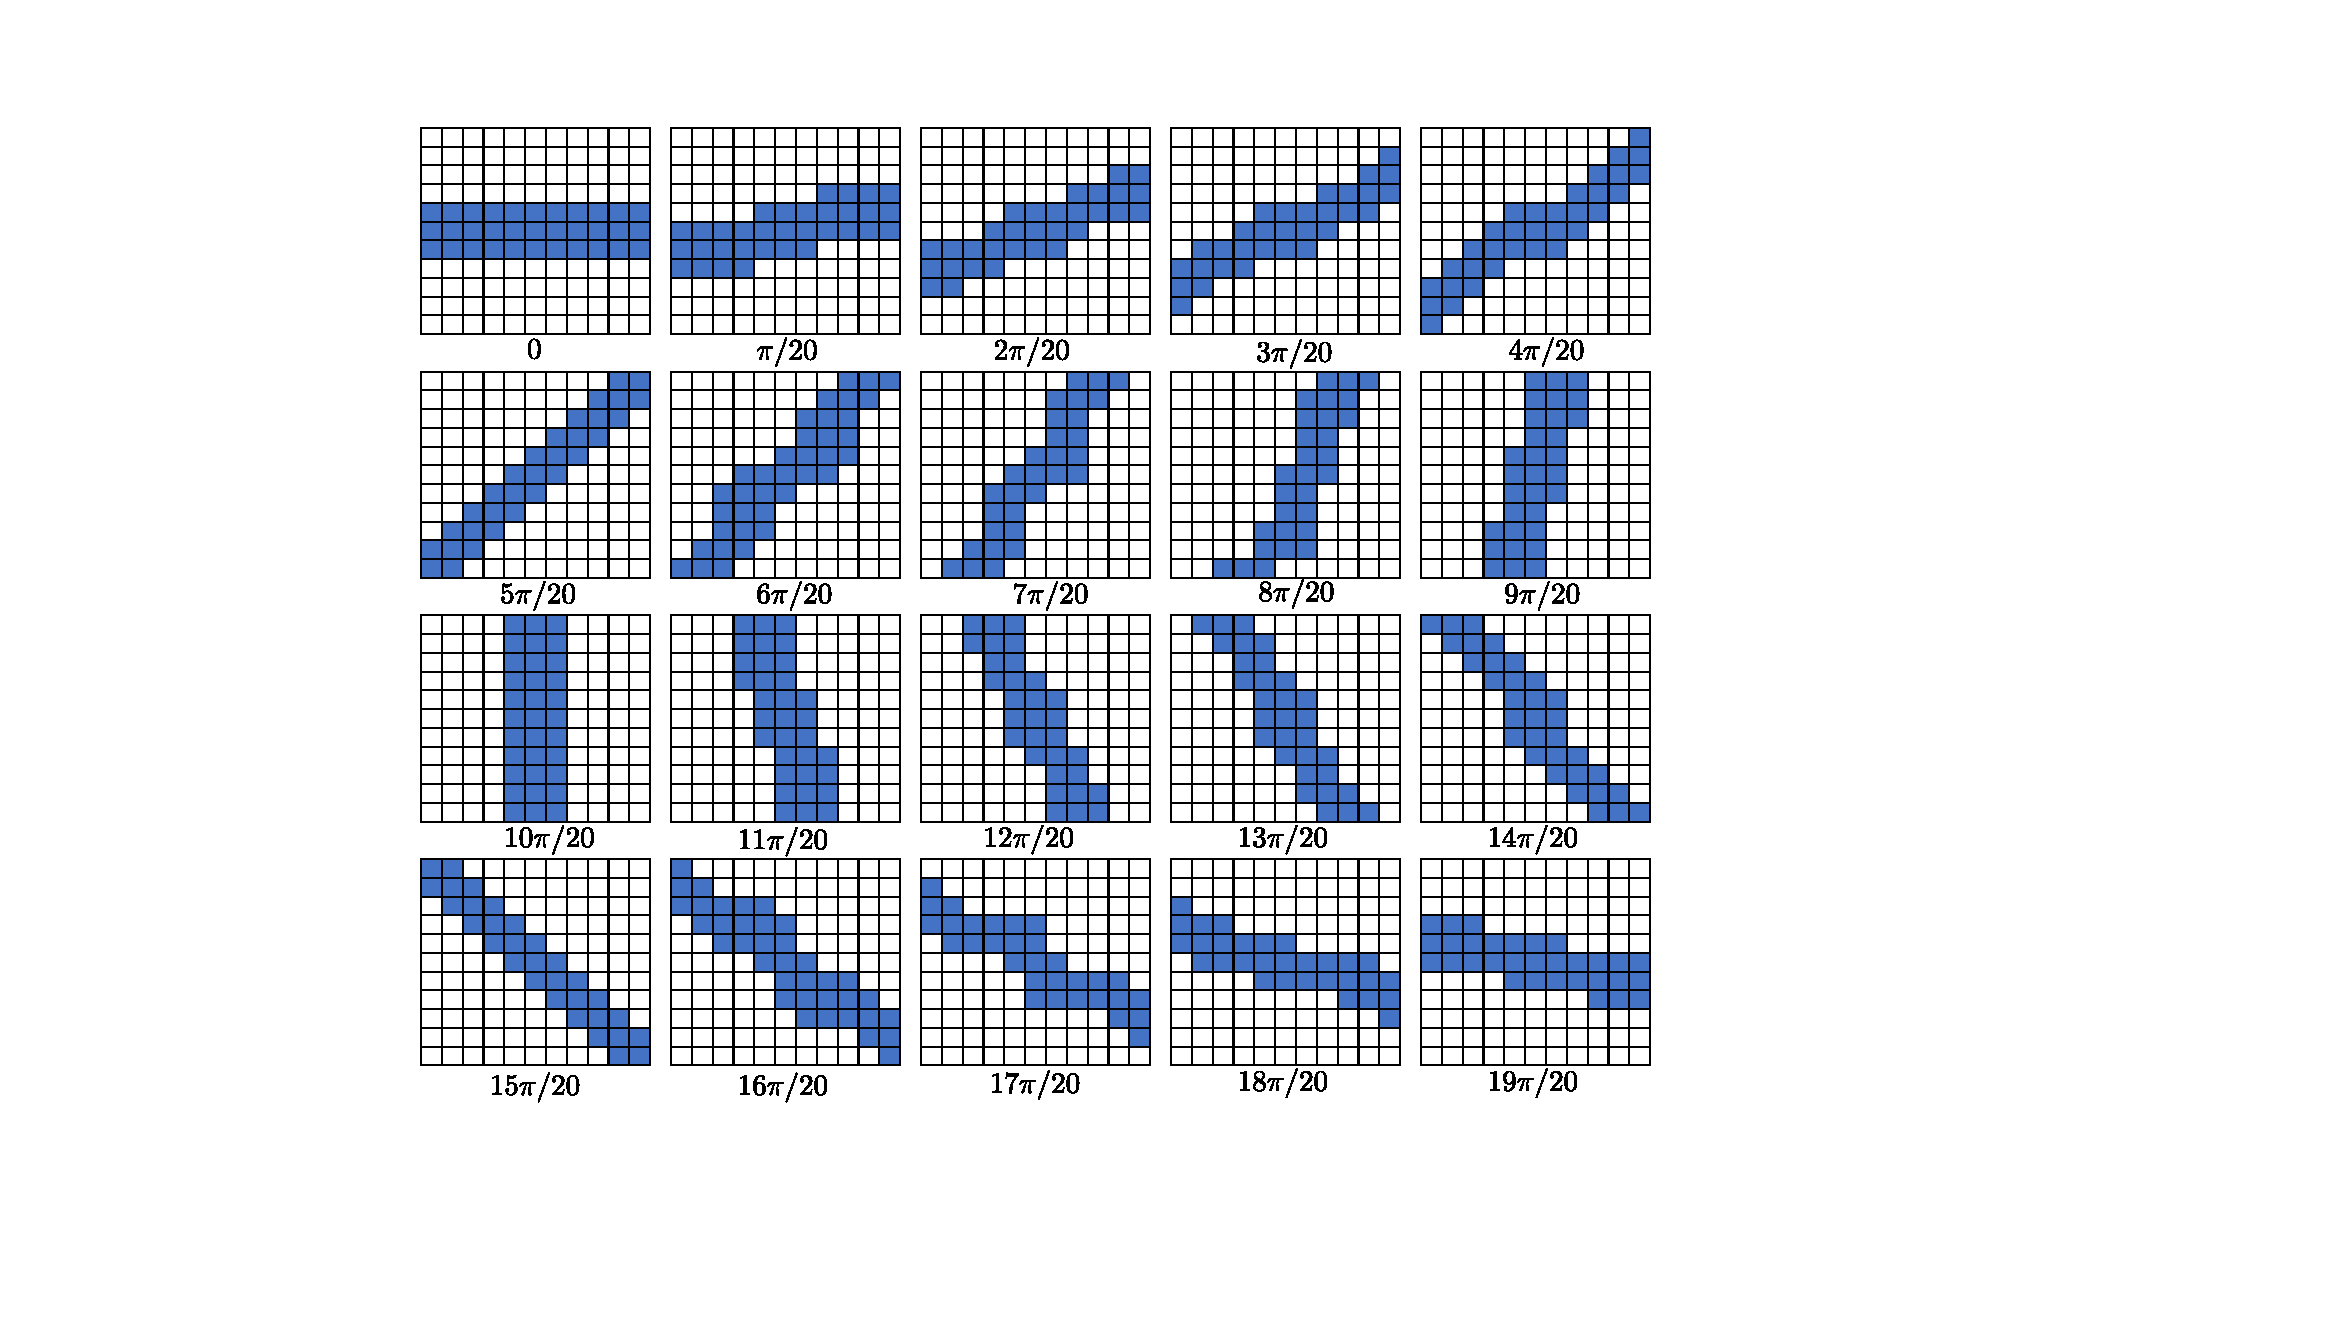
\includegraphics[width=0.8\textwidth]{Janelas_filtros_propostos}
	\caption{\textmd{Directional windows for the proposed filters}}
	\label{Janelas_filtros_propostos}
\end{figure}

For the TcNfilter, TcCfilter, and LInSARRFE filters, the phase limit $\psi_\xi$ is obtained based on the empirical models ($\mathcal{NT_C}$ and $\mathcal{CT_C}$), and on the physical model~\eqref{subsec:sec3.2.1_cap3Eq8}. 
To maintain the resolution, we propose applying the Mean Minimum Square Error (MMSE)~\cite{ImprovedSigmaFilterforSpeckleFilteringofSARImagery} estimator to the pixels selected in $\bm\psi_z'$ based on the phase limit:
\begin{equation}
	\widehat{\psi}_x=\overline{\bm\psi}_z'+b(\psi_z-\overline{\bm\psi}'_z),
\end{equation}
where $b=\big(\text{var}(\bm\psi_z')-\sigma^2_v\big)/\text{var}(\bm\psi_z')\in[0,1]$ is a weight, and  $\overline{\bm\psi}_z'$ and $\text{var}(\bm\psi_z')$ are the sample circular local mean and variance, and $\overline{\bm\psi}_v$ and $\sigma^2_v$ denote the circular mean and variance of the noise:
\begin{eqnarray}\label{subsec:sec3.7.2_cap3Eq5}
	\sigma^2_v = \int_{-\psi_\xi}^{\psi_\xi}(\psi-\overline{\bm\psi}_v)^2f(\psi)d\psi,~
	\overline{\bm\psi}_v=\int_{-\psi_\xi}^{\psi_\xi}\psi f(\psi)d\psi.
\end{eqnarray}

The proposed filters can be implemented following the steps outlined in the algorithm below.
\begin{algorithm}[hbt]
	\caption{Proposed Method: Steps}\label{proposed_method}
	\DontPrintSemicolon
	\SetKwInput{KwInput}{Input}
	\SetKwInput{KwOutput}{Output}
	\SetKwInput{KwCompute}{Compute}
	
	\KwInput{Interferometric image, standard model $F$: $\mathcal{NT}$, $\mathcal{CT}$, or~\eqref{subsec:sec3.2.1_cap3Eq8}, proportion $0<\xi\leq1$, threshold $\epsilon_{th}$ empirically defined}
	\KwOutput{Filtered image}
	
	\KwCompute{Filter each center pixel $\psi_c$ using an $11 \times 11$ window (Figure~\ref{Janelas_filtros_propostos})}
	
	Compute phase limit $\psi_\xi$ such that $F(\psi_\xi) - F(-\psi_\xi) = \xi$\;
	
	\For{each directional window}{
		Compute $|\langle e^{\mathrm{i}\bm{\psi}_\bullet}\rangle|$, where $\bm{\psi}_\bullet$ denotes the set of pixel values in each directional window\;
		\If{$|\langle e^{\mathrm{i}\bm{\psi}_\bullet}\rangle| < \epsilon_{th}$}{
			Recalculate the angle with IDW (Eqs. (6) and (7), Ref.~\cite{RefinedFilteringofInterferometricPhaseFromInSARData}) using a \(13 \times 13\) window\;
			Select the angle closest to $\widehat{\gamma}$\;
		}
		Subdivide into $3 \times 3$ subwindows, unwrap phase, sort pixels\;
		\If{$\psi_c < \psi_{(3)}$ \textbf{or} $\psi_c > \psi_{(7)}$}{
			The center pixel \( \psi_c \) is singular; therefore, replace it with the mean of $[\psi_{(3)}, \psi_{(7)}]$\;
		}
		Reject pixels outside $\psi_c - \psi_\xi < \psi_z \leq \psi_c + \psi_\xi$\;
		Compute local statistics: $\overline{\bm{\psi}}'_z$ and $\text{var}(\bm{\psi}'_z)$\;
		Compute the mean and variance of the noise: $\overline{\bm{\psi}}_v$ and $\sigma^2_v$\, respectively\;
		Compute weight $b$ and update $\widehat{\psi}_x$ using the MMSE estimator\;
	}
	\KwOutput{Return the filtered image}
\end{algorithm}
%
\section{Results}\label{sec:resu}

We used a Sentinel-1 SAR image (C--band) and a UAVSAR image (L--band). A simulated image was used to test the proposed approaches and compare them with well-established methods. First, we analyzed the simulated data, as described in Ref.~\cite{InSAR-MONet2022}. Thereafter, we analyzed the InSAR images from La Cumbre volcano, Los Alamos, and Robledo Volcano.

We measured the filters performance in the simulated dataset with Structural Similarity Index (SSIM), Root Mean Squared Error (RMSE), and Runtime (RT). 
More details about SSIM and RMSE can be found in~\cite{wbss_ssim, hastie2009elements}. 
This approach allows for an objective analysis of filtering quality, assessing the effectiveness of the methods in relation to noise-free data. 
For the SAR data, we used the number of residues (see Ref.~\cite{RS_Golg_zeb_wer}) and runtime (RT) as comparison criteria for the Refined InSAR Lee filter and the proposed methods.
The number of residues in the filtered image is always a good criterion for evaluating the effectiveness of InSAR phase filtering algorithms~\cite{EnhancedInterferometricPhaseNoiseFilteringoftheRefinedInSARFilter}, especially in scenarios where the clean phase is unknown.

For the application of filters based on physical models, the coherence map was generated from the noisy interferometric image, estimating the parameter $|\rho_c|$ at each image pixel by maximum likelihood, both for simulated and SAR data. 
As indicated in Ref.~\cite{RefinedFilteringofInterferometricPhaseFromInSARData}, the mean and standard deviation of the noise (Eqs. in~\eqref{subsec:sec3.7.2_cap3Eq5}) depend only on the coherence and the number of looks; therefore, we assumed $\theta = 0$, for more details see subsection~\ref{subsec:Coherence_est}. 
On the other hand, for the filters based on empirical models, the parameter $\mu$ was fixed at $\mu = 0$, while $\sigma$ was estimated using maximum likelihood.
After the filtering process, to restore phase information, we perform phase unwrapping~\cite{Fasttwodimensionalphaseunwrappingalgorithm}. 
Table~\ref{tab:filters_param} shows the setup parameters of the filters for each image. 

\begin{table}[hbt]
	\caption{Parameters Adopted for Each Filter in the Simulated and SAR Images.\label{tab:filters_param}}
	\begin{tabularx}{\textwidth}{
			l
			>{\centering\arraybackslash}X
			>{\centering\arraybackslash}X
			>{\centering\arraybackslash}X
			>{\centering\arraybackslash}X
		}
		\toprule
		\textbf{Filters} & 
		\textbf{\makecell{Simulated\\Data}} & 
		\textbf{\makecell{La Cumbre}} & 
		\textbf{\makecell{Los Alamos}} & 
		\textbf{\makecell{Robledo}} \\
		\midrule
		Refined Lee & $\theta=0$, $L=16$ & $\theta=0$, $L=16$ & $\theta=0$, $L=8$ & $\theta=0$, $L=8$ \\
		LInSARRFE    & $\theta=0$, $L=16$ & $\theta=0$, $L=16$ & $\theta=0$, $L=8$ & $\theta=0$, $L=8$  \\
		TcNfilter    & $\mu=0$ & $\mu=0$ & $\mu=0$ & $\mu=0$ \\
		TcCfilter    & $\mu=0$ & $\mu=0$ & $\mu=0$ & $\mu=0$  \\
		\bottomrule
	\end{tabularx}
\end{table}

%Phase unwrapping allows the reconstruction of phase continuity throughout space, eliminating phase jumps and providing a more accurate and useful representation of the information; for more information, see subsection~\ref{subsec:phase_unwrap}.



%
%############################ Aqui
%
\subsection{Simulated InSAR Data}
\label{simulated_data}

To evaluate the efficiency of the proposed methods, we used a simulated $128\times128$ pixel image. 
The Figure~\ref{Original_phase} was used as the reference (noise-free), while the Figure~\ref{Noise_phase} contains noise.

\begin{figure}[hbt]
	%\begin{adjustwidth}{-\extralength}{0cm}
	\centering
	\subfloat[\centering\label{Original_phase}]{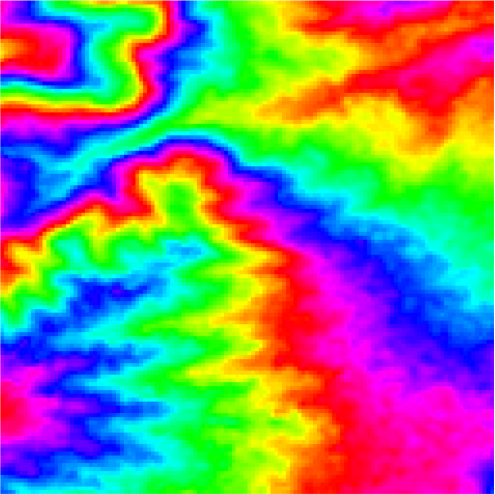
\includegraphics[width=.179\linewidth]{original_phase}}
	\hspace{0.01cm}
	\subfloat[\centering\label{Noise_phase}]{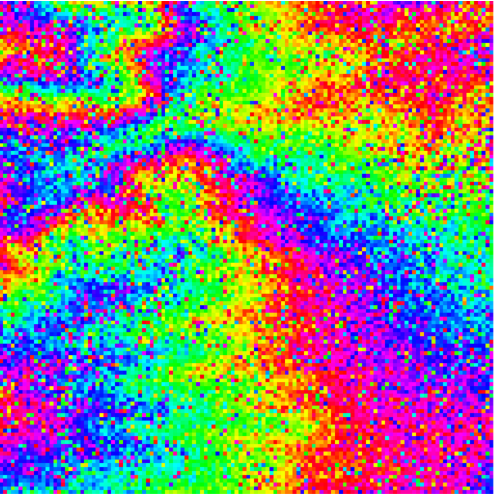
\includegraphics[width=.179\linewidth]{noise_phase}}
	\\
	\subfloat[\centering\label{LeeRefined}]{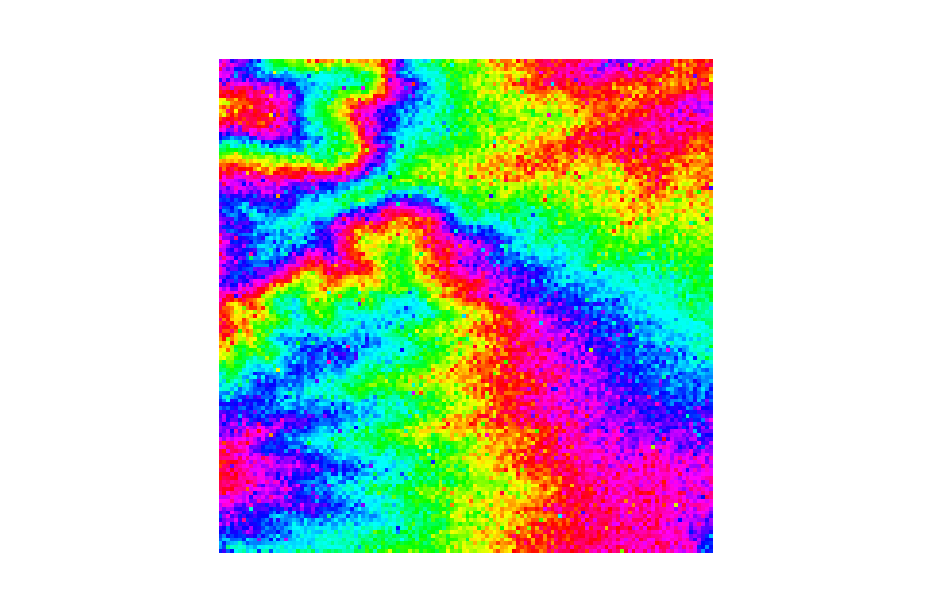
\includegraphics[width=.178\linewidth]{LeeRefined}}
	\hspace{0.01cm}
	\subfloat[\centering\label{LInSARRFE}]{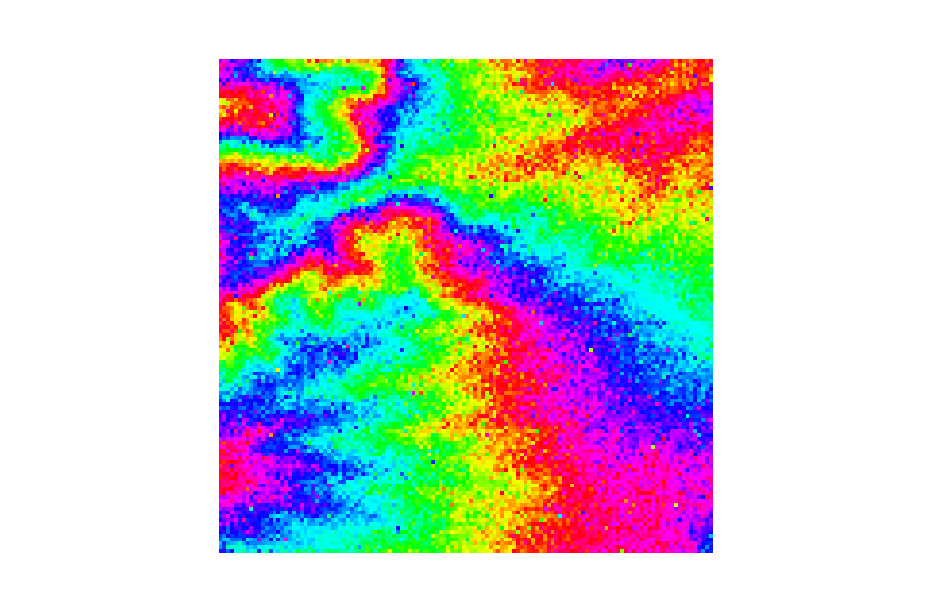
\includegraphics[width=.179\linewidth]{LInSARRFE}}
	\hspace{0.01cm}
	\subfloat[\centering\label{TcNfilter}]{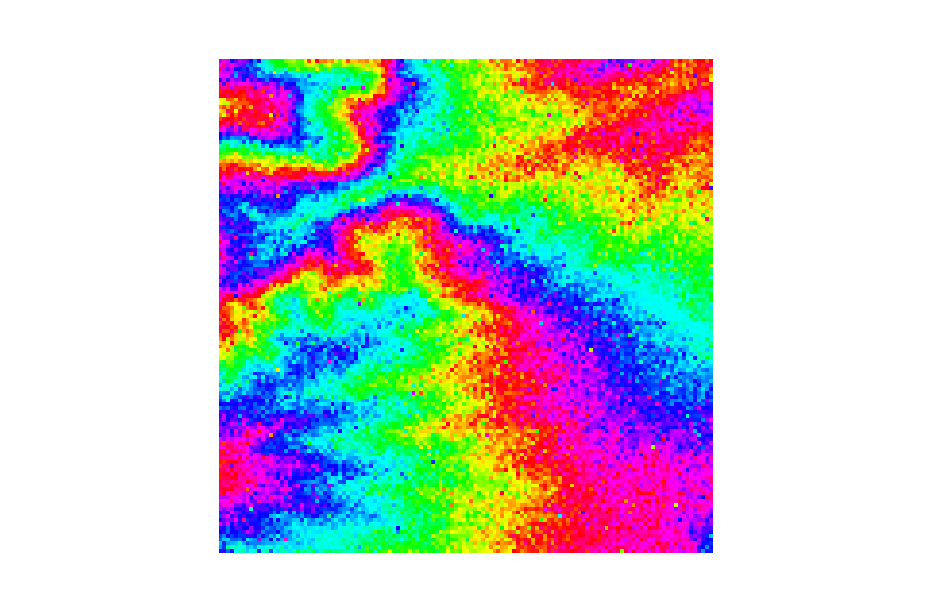
\includegraphics[width=.179\linewidth]{TcNfilter}}
	\hspace{0.01cm}
	\subfloat[\centering\label{TcCfilter}]{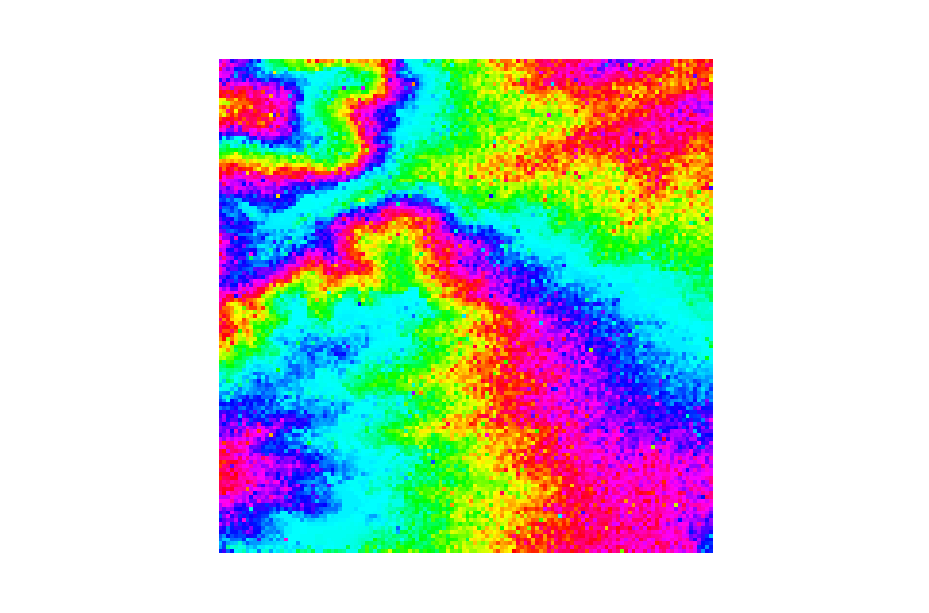
\includegraphics[width=.18\linewidth]{TcCfilter}}
	\\
	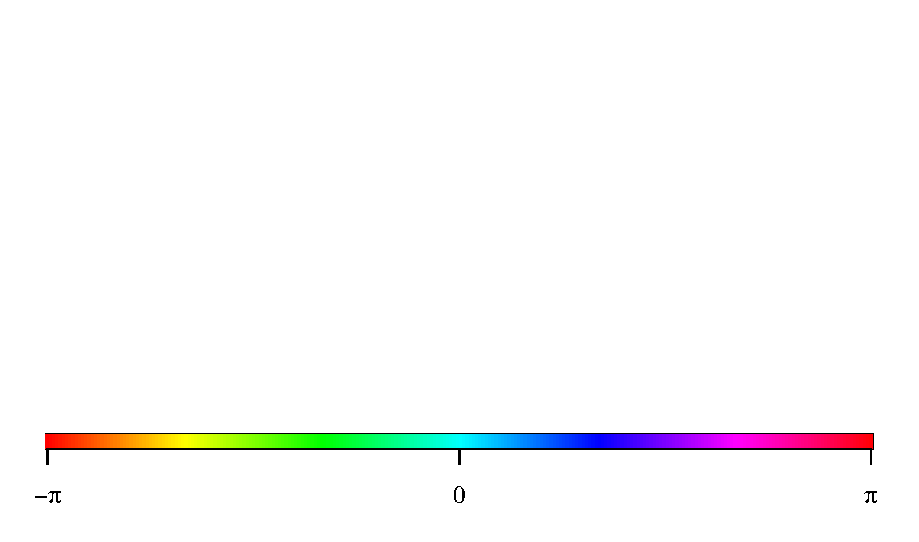
\includegraphics[width=.65\linewidth]{BarraCores}
	\\
	\subfloat[\centering\label{LeeRefined_unwrapped}]{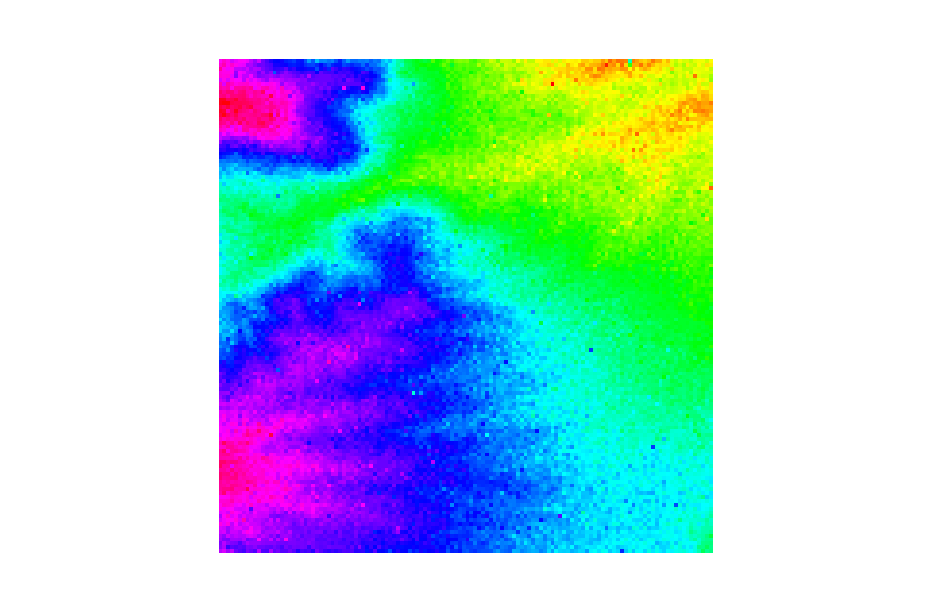
\includegraphics[width=.179\linewidth]{LeeRefined_unwrapped}}
	\hspace{0.01cm}
	\subfloat[\centering\label{LInSARRFE_unwrapped}]{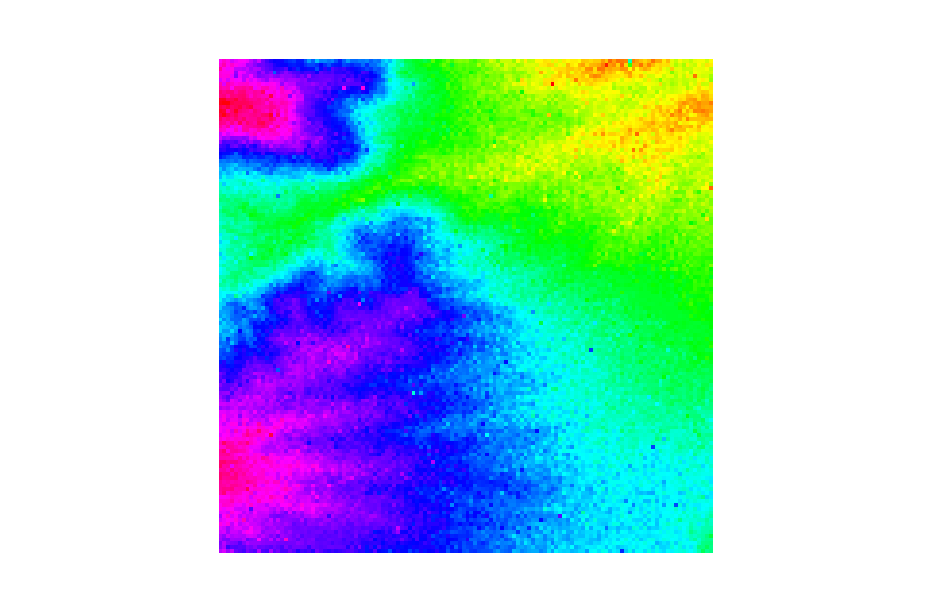
\includegraphics[width=.181\linewidth]{LInSARRFE_unwrapped}}
	\hspace{0.01cm}
	\subfloat[\centering\label{TcNfilter_unwrapped}]{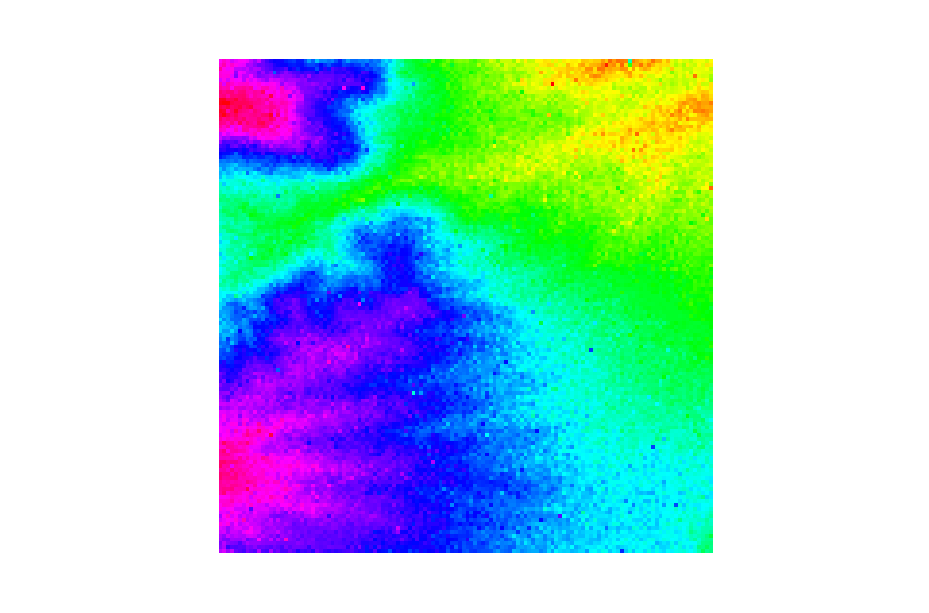
\includegraphics[width=.18\linewidth]{TcNfilter_unwrapped}}
	\hspace{0.01cm} 
	\subfloat[\centering\label{TcCfilter_unwrapped}]{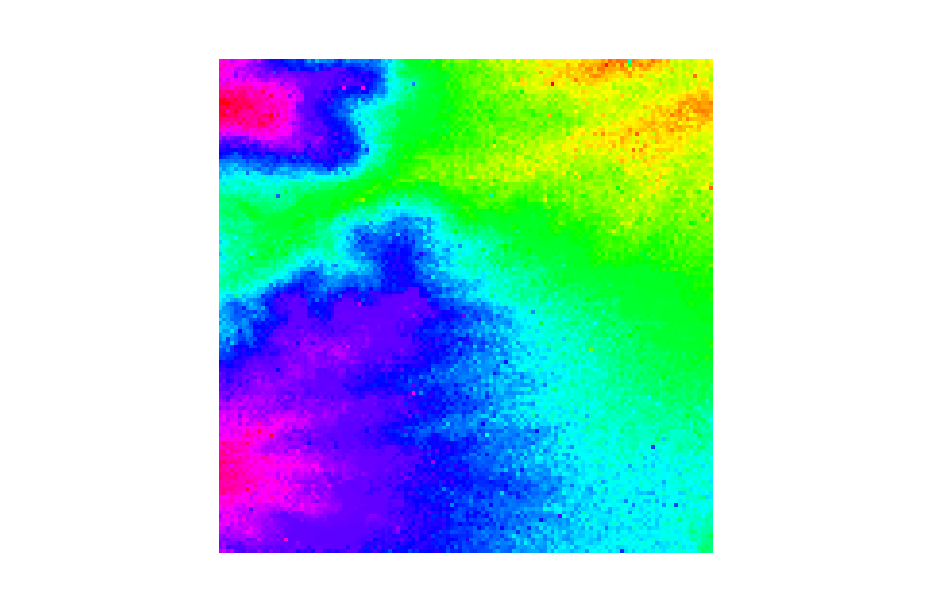
\includegraphics[width=.181\linewidth]{TcCfilter_unwrapped}}
	\\
	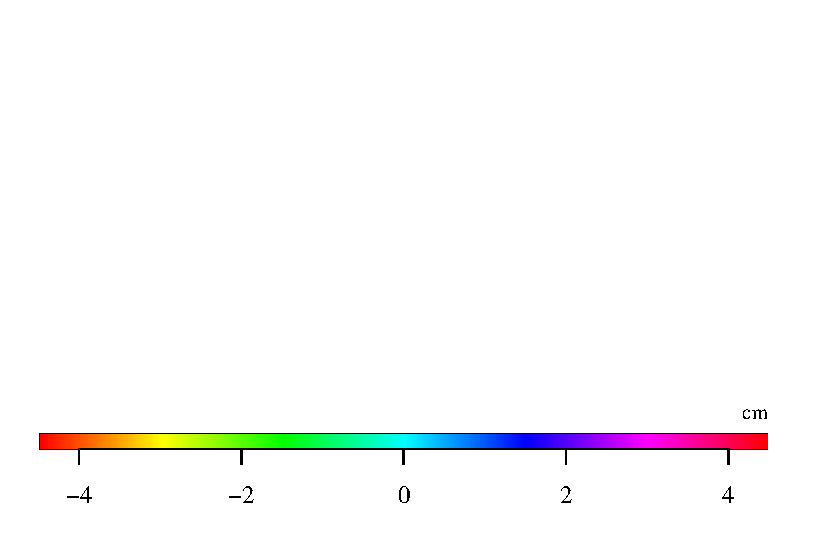
\includegraphics[width=.65\linewidth]{BarraCores_simu}
	%\end{adjustwidth}
	\caption{Before and after filtering: (\textbf{a})~Original Phase (pure), (\textbf{b})~Noisy Phase, (\textbf{c})~Refined Lee, (\textbf{d})~LInSARRFE, (\textbf{e})~TcNfilter, (\textbf{f})~TcCfilter. Unwrapped phase after filter application: (\textbf{g})~Refined Lee, (\textbf{h})~LInSARRFE, (\textbf{i})~TcNfilter, (\textbf{j})~TcCfilter}
	\label{img_simulada}
\end{figure}

As shown in Table~\ref{TabEficiencia_simu}, the TcCfilter exhibits the lowest mean RMSE and the highest accuracy among the analyzed filters across the $R = 30$ noise realizations. Additionally, the proposed filters LInSARRFE and TcNfilter present mean RMSE values that are only slightly higher than those of the Refined Lee filter.

\begin{table}[hbt]
	\caption{Efficiency of filters for simulated data: mean $\pm$ standard deviation over $R = 30$ independent noise realizations. Runtime (RT) values correspond to the average time among all replications. Time savings are computed relative to the Refined Lee; bold entries indicate the best value per column.\label{TabEficiencia_simu}}
	\begin{tabularx}{\textwidth}{
			l % Filter name (left-aligned)
			S[table-format=2.2] % Reserva 2 dígitos antes e 2 depois da vírgula
			S[table-format=2.2] % Reserva 2 dígitos antes e 2 depois da vírgula
			r
			S[table-format=2.2] % Reserva 2 dígitos antes e 2 depois da vírgula
			%>{\centering\arraybackslash}X  % TS
		}
		\toprule
		\textbf{Filter} & \textbf{RMSE (mean $\pm$ sd)} & \textbf{SSIM (mean $\pm$ sd)} & \textbf{RT (\si{\second})}&\textbf{Time Saved (\si{\percent})}\\
		\midrule
		Refined Lee  & $\mathbf{1.84038 \pm 6.8\cdot 10^{-3}}$        & $\mathbf{0.945286 \pm 4.1 \cdot 10^{-4}}$ & 5656.09 & $\text{---}$\\
		LInSARRFE & ${1.84926 \pm 4.7\cdot 10^{-3}}$        & ${0.944787 \pm 2.8\cdot 10^{-4}}$       & 624.82 & 88.95 \\
		TcNfilter & ${1.879114 \pm 6.6\cdot 10^{-3}}$        & ${0.943092 \pm 3.9\cdot 10^{-4}}$ & $\mathbf{343.78}$  & $\mathbf{93.92}$ \\
		TcCfilter & ${1.849049 \pm 4.6\cdot 10^{-3}}$ & ${0.944799\pm 2.7\cdot 10^{-4}}$ & 433.64  & 92.33 \\
		\bottomrule
	\end{tabularx}
\end{table}

The Kruskal-Wallis test applied to the 30-replication RMSE distributions yielded a statistically significant result for $H_0$: population medians are equal across filters, versus $H_1$: At least one distribution differs, with $\text{df} = 3$ degrees of freedom.
We obtained $p=0.000001 < 0.05$), confirming that the filters differ in their denoising accuracy.
   
Pairwise Wilcoxon signed-rank tests for $H_0$: difference of the median with respect to the Refined Lee's filter is zero versus $H_1$: the distributions differ
(using Bonferroni-corrected $\alpha_{\text{adj}} = 0.01667$) showed that TcCfilter achieves a significantly lower RMSE ($p=0.000002 < 0.017$), and LInSARRFE and TcNfilter show similar results.
%All alternative filters differ significantly from the Refined Lee's for RMSE and SSIM.

Regarding SSIM, the metric that evaluates the structural similarity between the filtered interferogram and the reference image (noise-free)~\cite{ANonlocalFilterforSARInterferometric}, the Refined Lee filter shows a slight advantage, with a value closer to $1$. 
The proposed filters, especially LInSARRFE and TcCfilter, exhibit SSIM values very close to those of the Refined Lee filter, indicating no significant loss in preserving image structure. 

Regarding runtime, the proposed filters significantly outperform the Refined Lee filter, which has the longest processing times, potentially restricting its use in time-sensitive applications. 
Notably, the TcNfilter achieves the greatest time savings, resulting in an approximate time reduction of 
\qty{93.92}{\percent}. 
In contrast, the slow processing of the Refined Lee filter limits its practical applicability. 
Therefore, the proposed filters excel over the Refined Lee filter in terms of processing efficiency.

\subsection{La Cumbre data}
\label{LaCumbre}
%We analyzed data from the eruption of the La Cumbre volcano on Fernandina Island in the Galapagos archipelago, Ecuador, on January 12, 2020. The Region of Interest (ROI) presented in Figure~\ref{interferograma_LaCumbe} has $346\times492$ pixels.
Figures~\ref{img_LeeRefined}, \ref{img_LInSARRFE}, \ref{img_TcNfilter}, and~\ref{img_TcCfilter} show the results of applying the Refined Lee InSAR, LInSARRFE, TcNfilter, and TcCfilter filters. Figures~\ref{unwrap_phase_LeeRefined}, \ref{unwrap_phase_LInSARRFE}, \ref{unwrap_phase_TcNfilter}, and~\ref{unwrap_phase_TcCfilter} show the unwrapped phases.

\begin{figure}[hbt]
	%\begin{adjustwidth}{-\extralength}{0cm}
	\centering
	\subfloat[\centering\label{interferograma_LaCumbe}]{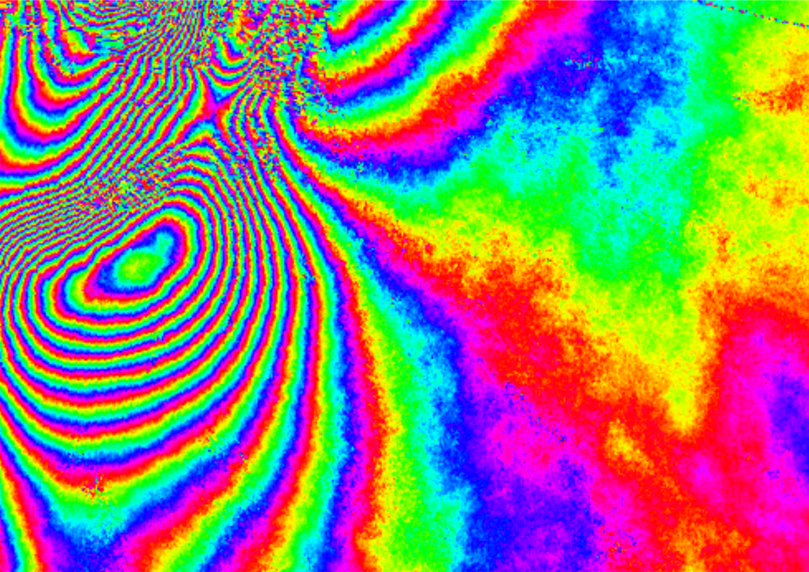
\includegraphics[width=.199\linewidth]{interferograma_LaCumbe}}
	\\
	%\subfloat[ \label{img_medianFilter}]{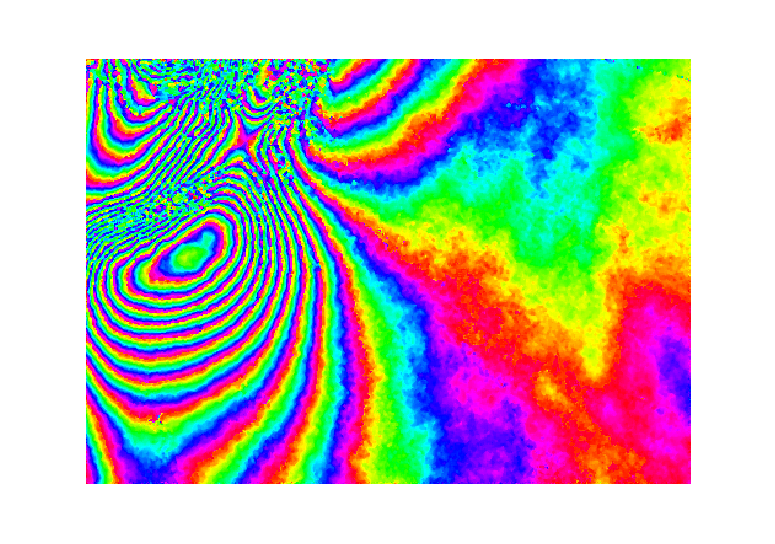
\includegraphics[width=.179\linewidth]{img_medianFilter}}
	\hspace{0.01cm}
	\subfloat[\centering\label{img_LeeRefined}]{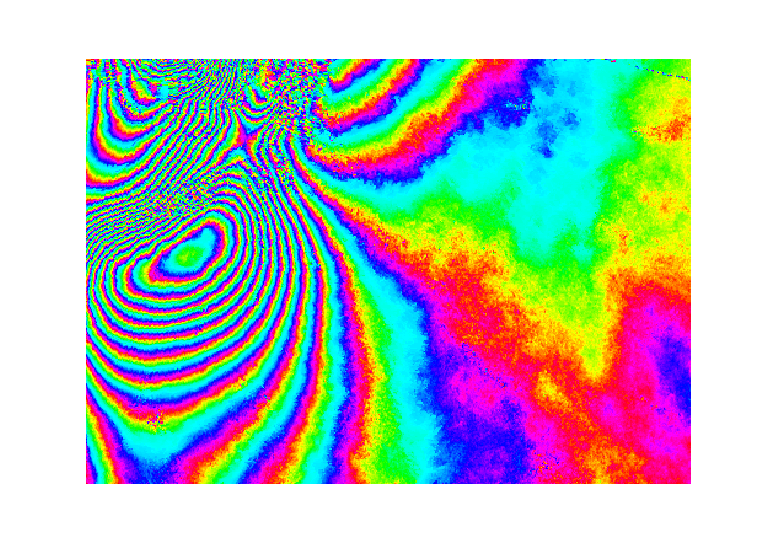
\includegraphics[width=.198\linewidth]{img_LeeRefined}}
	\hspace{0.01cm}
	\subfloat[\centering\label{img_LInSARRFE}]{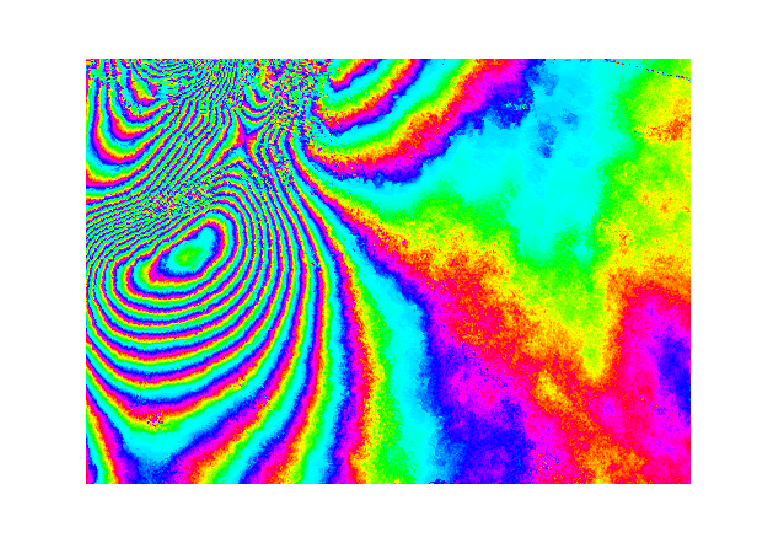
\includegraphics[width=.199\linewidth]{img_LInSARRFE}}
	\hspace{0.01cm}
	\subfloat[\centering\label{img_TcNfilter}]{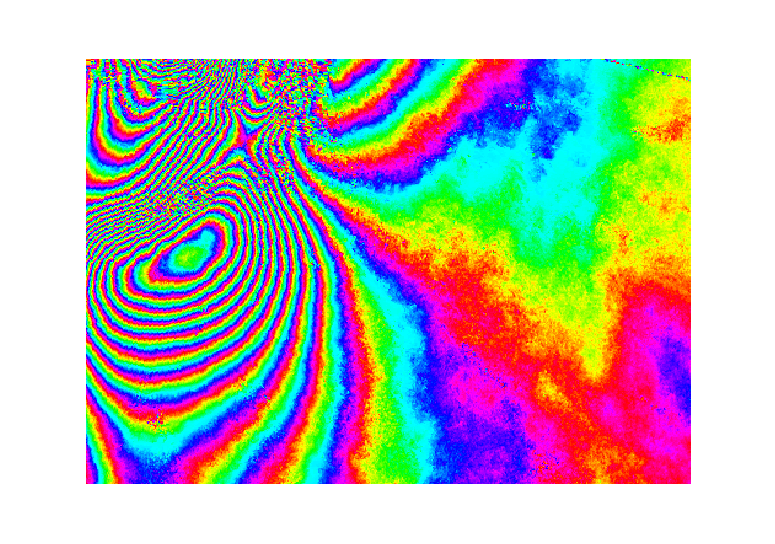
\includegraphics[width=.199\linewidth]{img_TcNfilter}}
	\hspace{0.01cm}
	\subfloat[\centering\label{img_TcCfilter}]{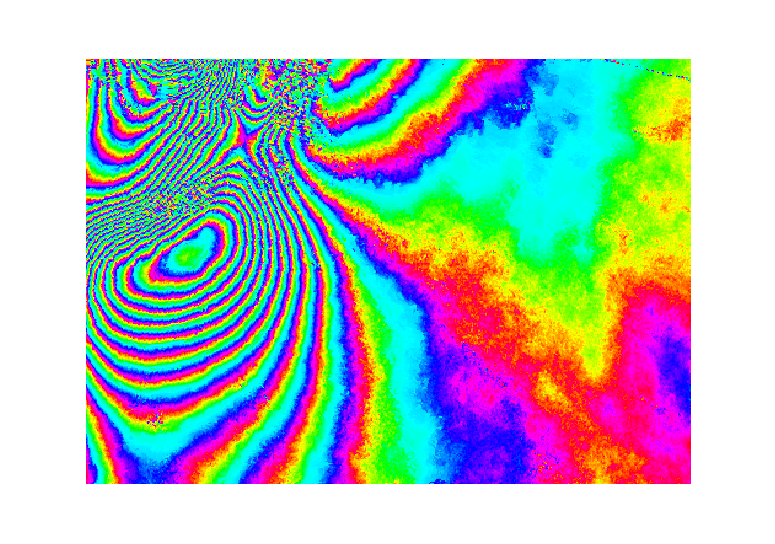
\includegraphics[width=.20\linewidth]{img_TcCfilter}}
	\\
	%\vspace{-0.3cm}
	{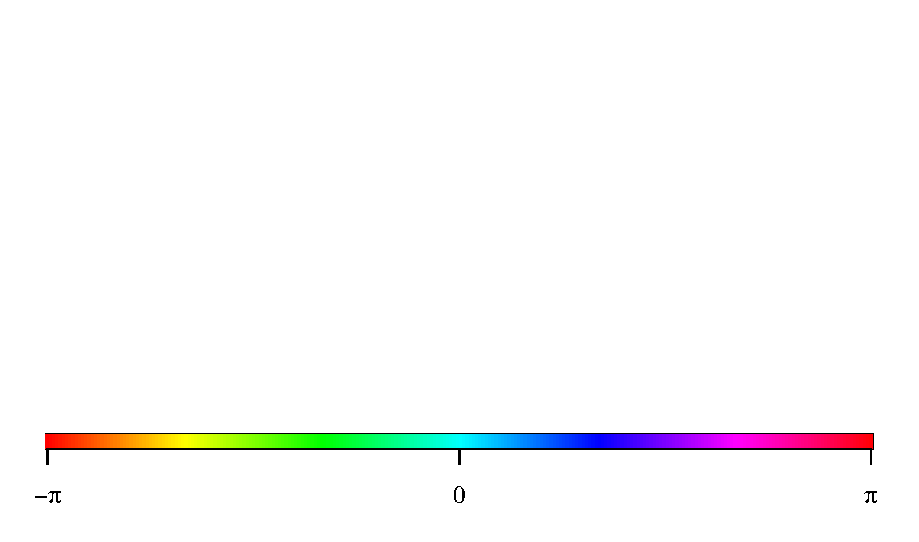
\includegraphics[width=.67\linewidth]{BarraCores}}
	\\	
	%\subfloat[ \label{unwrap_phase_median}]{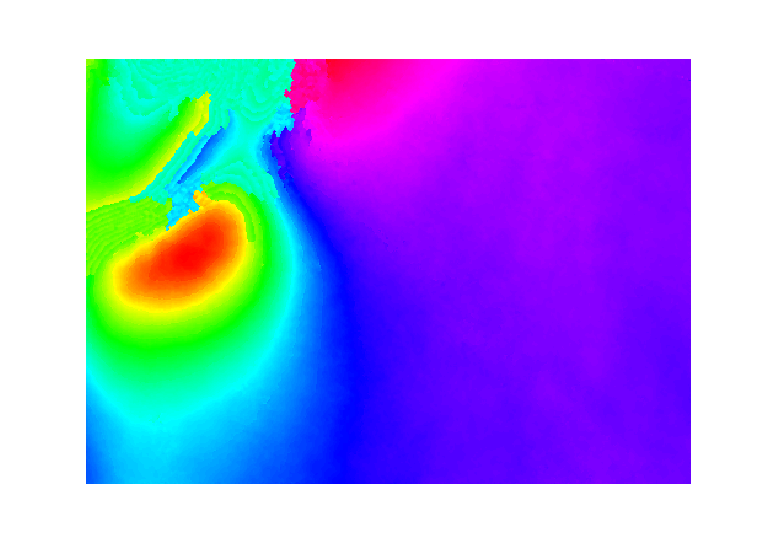
\includegraphics[width=.181\linewidth]{unwrap_medianFilter}}
	\hspace{0.01cm}
	\subfloat[\centering\label{unwrap_phase_LeeRefined}]{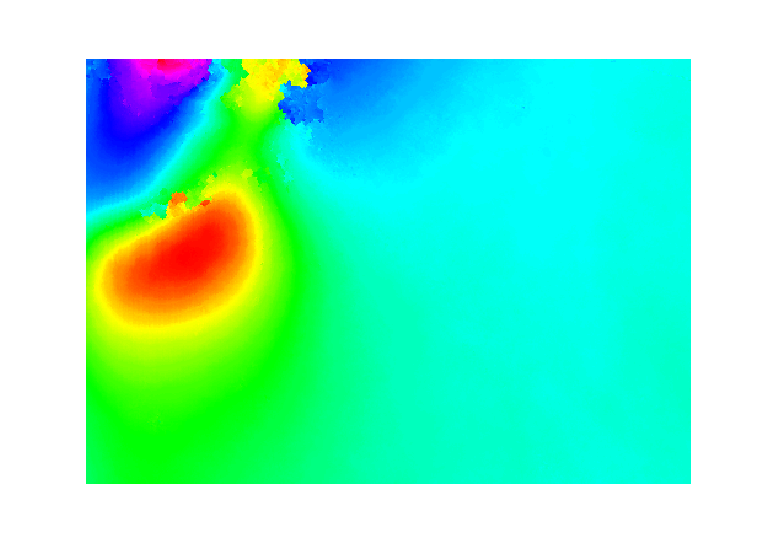
\includegraphics[width=.199\linewidth]{unwrap_LeeRefined_0705.2}}
	\hspace{0.01cm}
	\subfloat[\centering\label{unwrap_phase_LInSARRFE}]{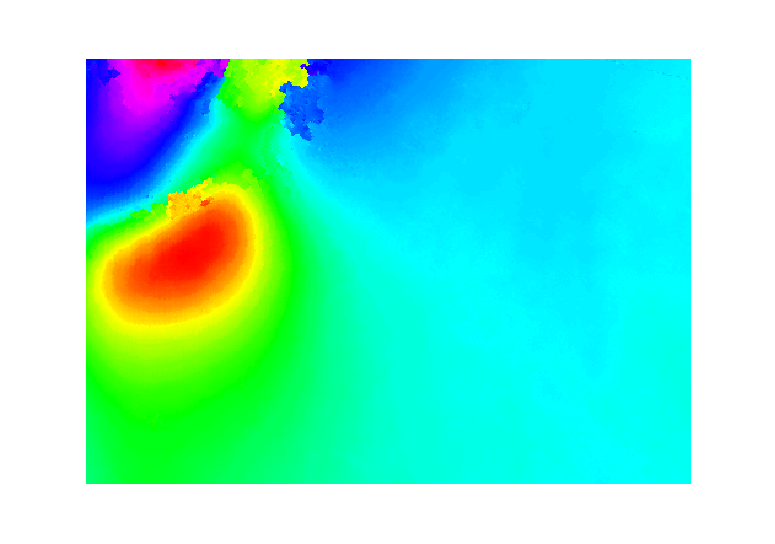
\includegraphics[width=.201\linewidth]{unwrap_LInSARRFE_0705}}
	\hspace{0.01cm}
	\subfloat[\centering\label{unwrap_phase_TcNfilter}]{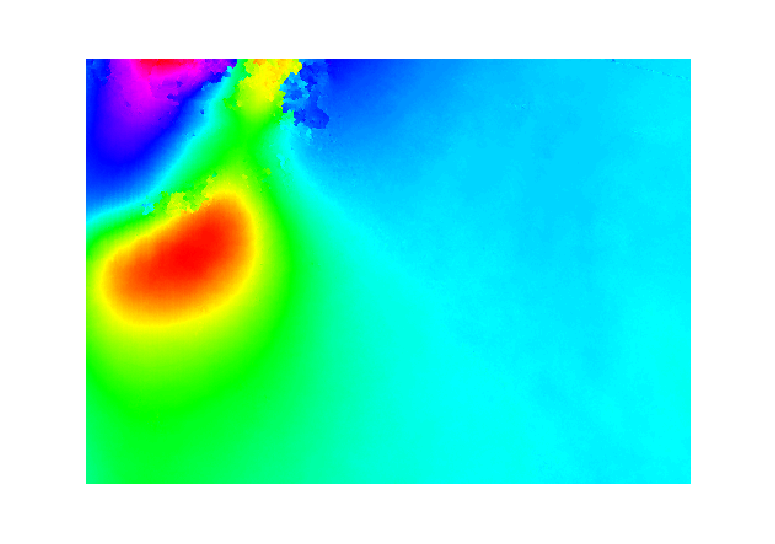
\includegraphics[width=.20\linewidth]{unwrap_TcNfilter-1_01}}
	\hspace{0.01cm} 
	\subfloat[\centering\label{unwrap_phase_TcCfilter}]{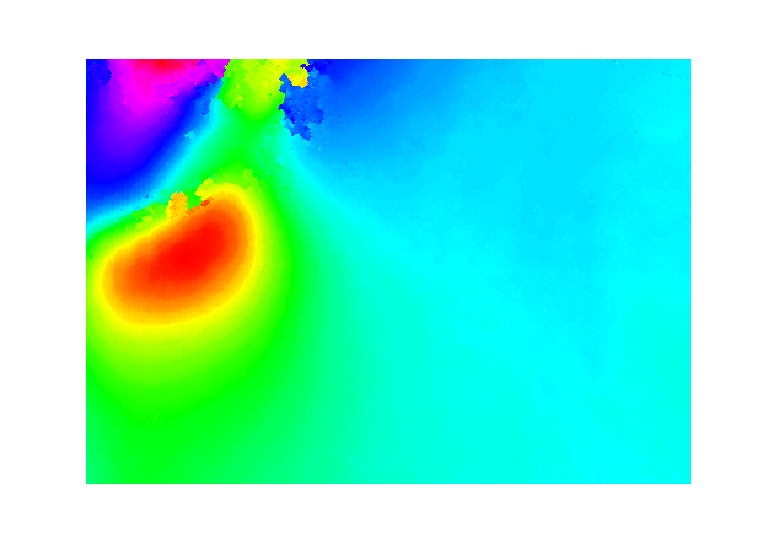
\includegraphics[width=.201\linewidth]{unwrap_TcCfilter-1-03}}
	\\
	\vspace{-0.3cm}
	\subfloat{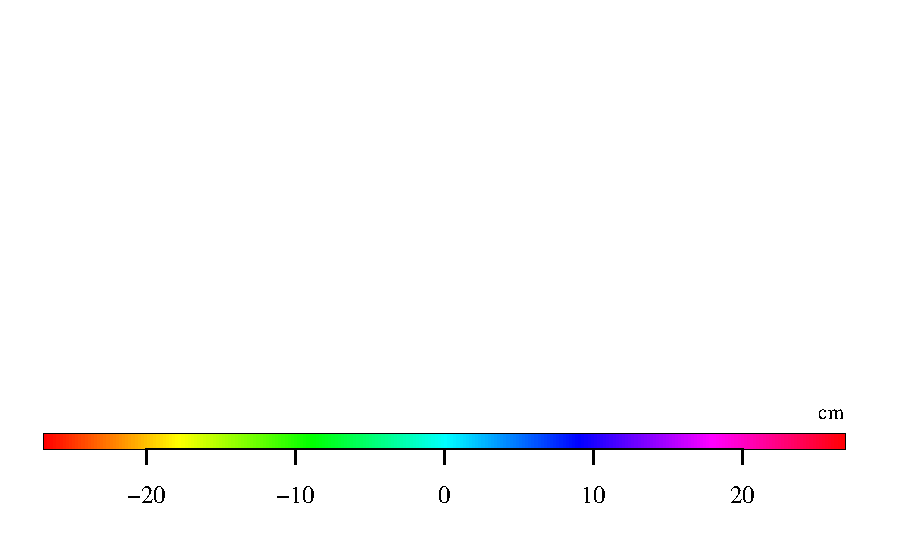
\includegraphics[width=.67\linewidth]{BarraCores_unwrap1}}
	%\end{adjustwidth}
	%\caption{\textmd{Interferograms filtered and before unwrapping the phase (top) and after unwrapping (bottom)}}
	\caption{La Cumbre image before and after filtering: (\textbf{a})~Unfiltered Phase, (\textbf{b})~Refined Lee, (\textbf{c})~LInSARRFE, (\textbf{d})~TcNfilter, (\textbf{e})~TcCfilter. Unwrapped phase after filter application: (\textbf{f})~Refined Lee, (\textbf{g})~LInSARRFE, (\textbf{h})~TcNfilter, (\textbf{i})~TcCfilter}
	\label{filters1_la_cumbre} % label da figura toda
\end{figure}

Based on the data presented in Table~\ref{TabSAREficiencia}, the Refined Lee filter significantly reduces the number of residues, achieving a reduction of 
\qty{79}{\percent}, 
which highlights its effective filtering capability. 
However, this filter has the longest runtime, potentially limiting its applicability in time-sensitive scenarios. 
In contrast, the LInSARRFE filter demonstrates the greatest reduction in residues among the evaluated filters, with an approximate reduction of 
\qty{82}{\percent}. 
Additionally, its runtime is significantly shorter than that of the Refined Lee filter, resulting in a 
\qty{79}{\percent} reduction in processing time.

The filters based on empirical models, TcNfilter and TcCfilter, yielded the same residual reduction ($\qty{79}{\percent}$), but they stand out for their computational efficiency. 
%Therefore, the filters have equivalent performance in reducing residues.
The TcNfilter is the fastest, with a $\qty{97}{\percent}$ reduction in runtime, while the TcCfilter also demonstrates excellent performance, achieving a $\qty{96}{\percent}$ reduction in runtime. 
These results indicate that the proposed filters offer an effective balance between filtering quality and computational efficiency, making them viable alternatives to the Refined Lee filter in scenarios that require both speed and accuracy. 

\begin{table}[hbt]
	\caption{Efficiency of filters for SAR data -- La Cumbre.\label{TabSAREficiencia}}
	\begin{tabularx}{\textwidth}{
			l % Filter name
			>{\centering\arraybackslash}X % Number of Residues
			>{\centering\arraybackslash}X % Reduction of residues (%)
			>{\centering\arraybackslash}X % RT (s)
			>{\centering\arraybackslash}X % Time Saved (%)
		}
		\toprule
		\textbf{Filter} & \textbf{\makecell{Number of\\ Residues}} & \textbf{\makecell{Reduction of \\ Residues (\%)}} & \textbf{RT (s)} & \textbf{\makecell{Time\\ Saved (\%)}} \\
		\midrule
		Unfiltered  & 11838     & --- & ---        & --- \\
		Refined Lee    & 2481      & 79.04 & 57851.37  & --- \\
		LInSARRFE   & \textbf{2145}  & \textbf{81.88} & 12069.78 & 79.02 \\
		TcNfilter   & 2432      & 79.45 & \textbf{2023.66} & 96.50 \\
		TcCfilter   & 2428      & 79.49 & 2436.25       & 95.78 \\
		\bottomrule
	\end{tabularx}
\end{table}
%
\subsection{Los Alamos Data}\label{Los_Alamos_data}
Table~\ref{TabSAR_Los_Alamos} shows the results of the filters. 
The second column shows the number of residues, and the third column shows the percentage reduction in residues compared to the unfiltered image. Likewise, the fourth column shows the runtime as a percentage of the refined Lee runtime.

\begin{table}[hbt]
	\caption{Efficiency of filters for SAR data -- Los Alamos.\label{TabSAR_Los_Alamos}}
	\begin{tabularx}{\textwidth}{
			l % Filter name
			>{\centering\arraybackslash}X % Number of Residues
			>{\centering\arraybackslash}X % Reduction of residues (%)
			>{\centering\arraybackslash}X % RT (s)
			>{\centering\arraybackslash}X % Time Saved (%)
		}
		\toprule
		\textbf{Filter} & \textbf{\makecell{Number of\\ Residues}} & \textbf{\makecell{Reduction of \\ Residues (\%)}} & \textbf{RT (s)} & \textbf{\makecell{Time\\ Saved (\%)}} \\
		\midrule
		Unfiltered  & 12687     & --- & ---        & --- \\
		Refined Lee    & 4581      & 63.09 & 6021.06  & --- \\
		LInSARRFE   & 4801  	& 62.15 & 1642.30 & 72.72 \\
		TcNfilter   & 4881      & 61.52 & \textbf{1369.55} & 77.25 \\
		TcCfilter   & \textbf{4424}     & \textbf{65.12} & 1408.87       & 76.60 \\
		\bottomrule
	\end{tabularx}
\end{table}

Figures~\ref{img_LeeRefined_alamos}, \ref{img_LInSARRFE_alamos}, \ref{img_TcNfilter_alamos}, and~\ref{img_TcCfilter_alamos} show the results after applying the Refined Lee InSAR, LInSARRFE, TcNfilter, and TcCfilter filters. Figures~\ref{unwrap_LeeRefined_alamos}, \ref{unwrap_LInSARRFE_alamos}, \ref{unwrap_TcNfilter_alamos}, and~\ref{unwrap_TcCfilter_alamos} show their unwrapped phases.
\begin{figure}[hbt]
	%\begin{adjustwidth}{-\extralength}{0cm}
	\centering
	\subfloat[\centering\label{InSAR_alamos}]{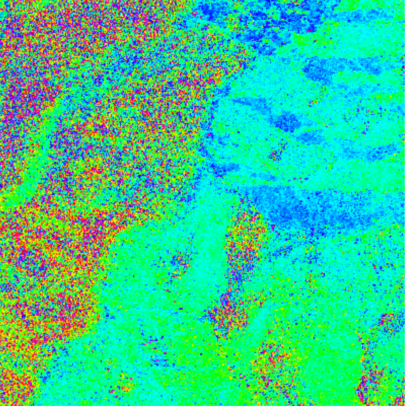
\includegraphics[width=.20\linewidth]{InSAR_alamos}}
	\\
	%\subfloat[ \label{img_medianFilter}]{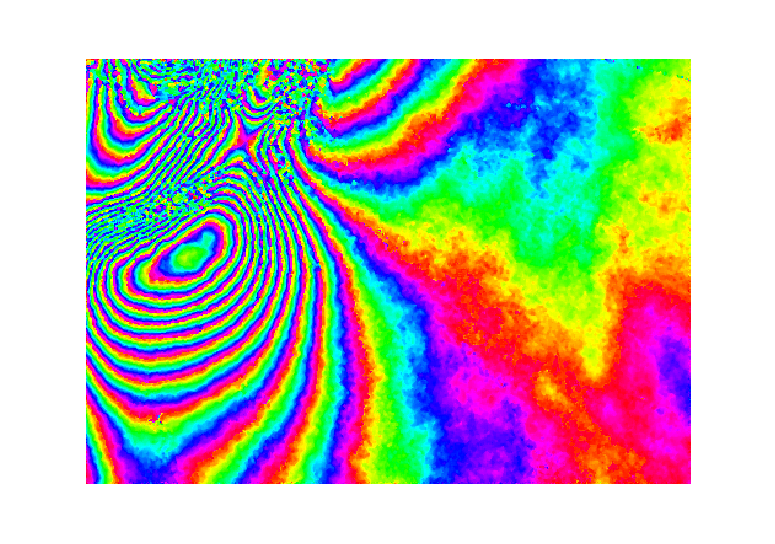
\includegraphics[width=.179\linewidth]{img_medianFilter}}
	\hspace{0.01cm}
	\subfloat[\centering\label{img_LeeRefined_alamos}]{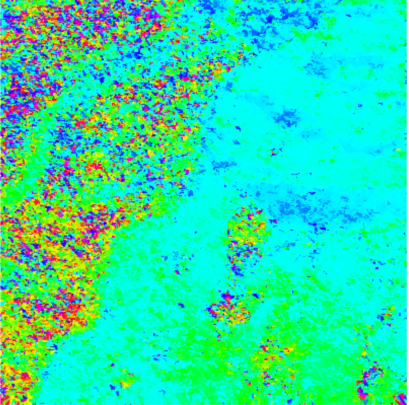
\includegraphics[width=.202\linewidth]{img_LeeRefined_alamos}}
	\hspace{0.01cm}
	\subfloat[\centering\label{img_LInSARRFE_alamos}]{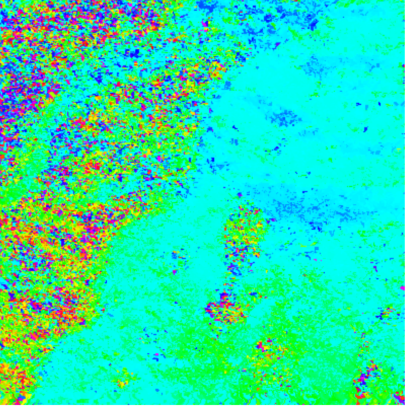
\includegraphics[width=.20\linewidth]{img_LInSARRFE_alamos}}
	\hspace{0.01cm}
	\subfloat[\centering\label{img_TcNfilter_alamos}]{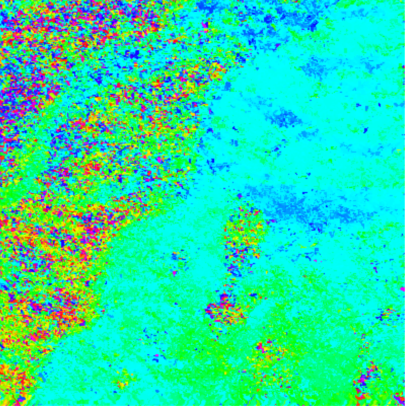
\includegraphics[width=.20\linewidth]{img_TcNfilter_alamos}}
	\hspace{0.01cm}
	\subfloat[\centering\label{img_TcCfilter_alamos}]{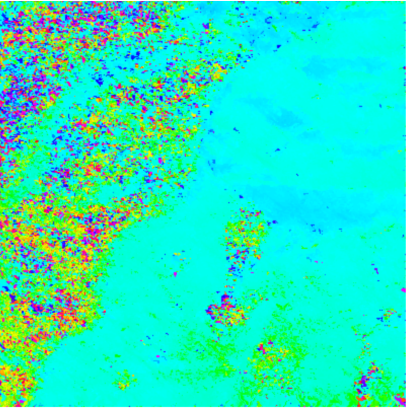
\includegraphics[width=.20\linewidth]{img_TcCfilter_alamos}}
	\\
	{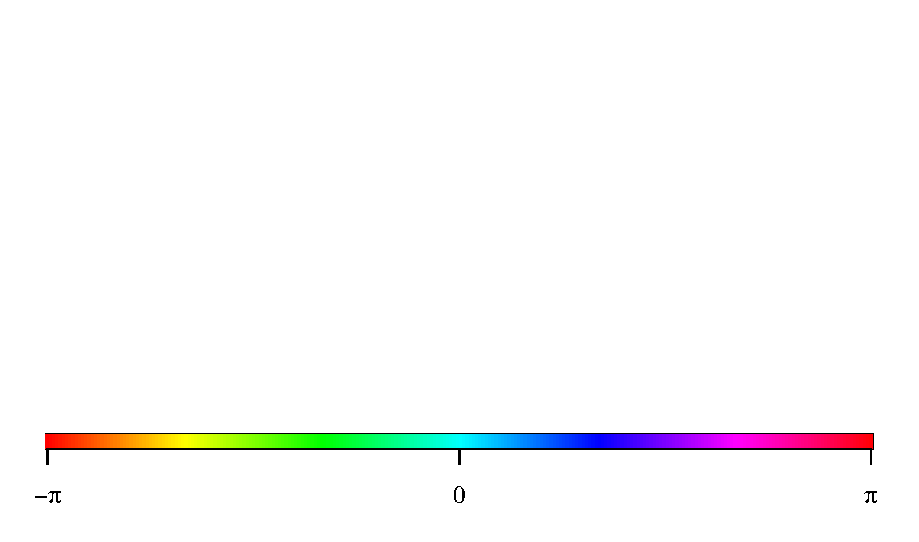
\includegraphics[width=.67\linewidth]{BarraCores}}
	\\	
	\hspace{0.01cm}
	\subfloat[\centering\label{unwrap_LeeRefined_alamos}]{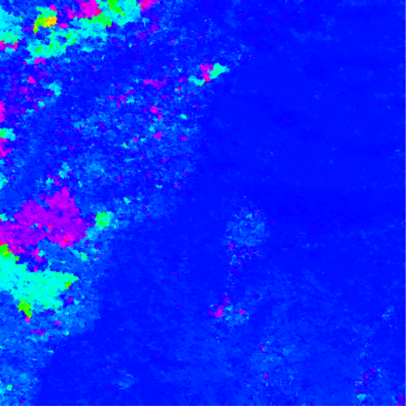
\includegraphics[width=.2\linewidth]{unwrap_LeeRefined_alamos}}
	\hspace{0.01cm}
	\subfloat[\centering\label{unwrap_LInSARRFE_alamos}]{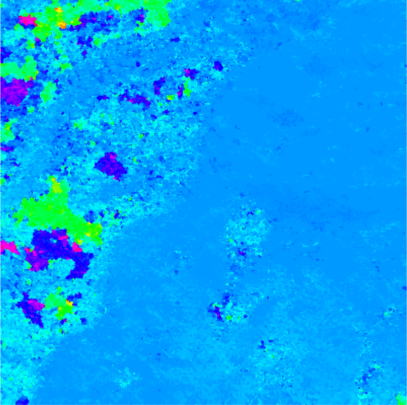
\includegraphics[width=.201\linewidth]{unwrap_LInSARRFE_alamos}}
	\hspace{0.01cm}
	\subfloat[\centering\label{unwrap_TcNfilter_alamos}]{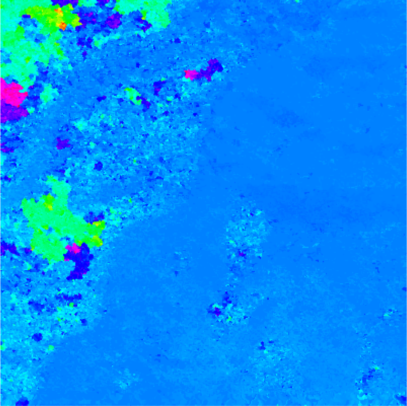
\includegraphics[width=.20\linewidth]{unwrap_TcNfilter_alamos}}
	\hspace{0.01cm} 
	\subfloat[\centering\label{unwrap_TcCfilter_alamos}]{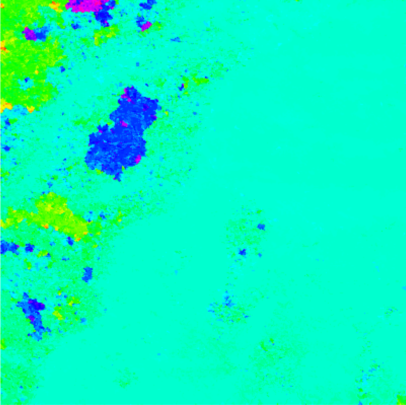
\includegraphics[width=.201\linewidth]{unwrap_TcCfilter_alamos}}
	\\
	\vspace{-0.3cm}
	\subfloat{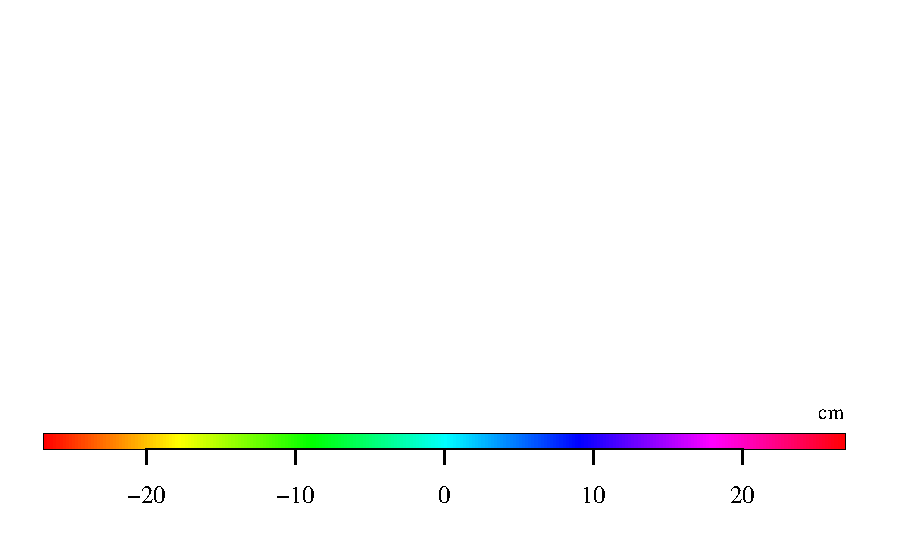
\includegraphics[width=.67\linewidth]{BarraCores_unwrap1}}
	%\end{adjustwidth}
	%\caption{\textmd{Interferograms filtered and before unwrapping the phase (top) and after unwrapping (bottom)}}
	\caption{Los Alamos image before and after filtering: (\textbf{a})~Unfiltered Phase, (\textbf{b})~Refined Lee, (\textbf{c})~LInSARRFE, (\textbf{d})~TcNfilter, (\textbf{e})~TcCfilter. Unwrapped phase after filter application: (\textbf{f})~Refined Lee, (\textbf{g})~LInSARRFE, (\textbf{h})~TcNfilter, (\textbf{i})~TcCfilter}
	\label{filters_los_alamos} % label da figura toda
\end{figure}
%
\subsection{Robledo Volcano Data}\label{Robledo_Volcano_data}
Table~\ref{TabSAR_Robledo} has the same data as the previous table for the Robledo volcano InSAR image.
\begin{table}[hbt]
	\caption{Efficiency of filters for SAR data -- Robledo.\label{TabSAR_Robledo}}
	\begin{tabularx}{\textwidth}{
			l % Filter name
			>{\centering\arraybackslash}X % Number of Residues
			>{\centering\arraybackslash}X % Reduction of residues (%)
			>{\centering\arraybackslash}X % RT (s)
			>{\centering\arraybackslash}X % Time Saved (%)
		}
		\toprule
		\textbf{Filter} & \textbf{\makecell{Number of\\ Residues}} & \textbf{\makecell{Reduction of \\ Residues (\%)}} & \textbf{RT (s)} & \textbf{\makecell{Time\\ Saved (\%)}} \\
		\midrule
		Unfiltered  & 25080     & --- & ---        & --- \\
		Refined Lee    & 8704      & 65.29 & 6540.03  & --- \\
		LInSARRFE   & 9205  	& 63.30 & 1601.69 & 75.51 \\
		TcNfilter   & 9339      & 62.76 & \textbf{1390.55} & 78.74 \\
		TcCfilter   & \textbf{8476}     & \textbf{66.20} & 1433.03       & 78.09 \\
		\bottomrule
	\end{tabularx}
\end{table}

Figures~\ref{img_LeeRefined_ArgVol}, \ref{img_LInSARRFE_ArgVol}, \ref{img_TcNfilter_ArgVol}, and~\ref{img_TcCfilter_ArgVol} show the results after applying the Refined Lee InSAR, LInSARRFE, TcNfilter, and TcCfilter filters. Figures~\ref{unwrap_LeeRefined_ArgVol}, \ref{unwrap_LInSARRFE_ArgVol}, \ref{unwrap_TcNfilter_ArgVol}, and~\ref{unwrap_TcCfilter_ArgVol} show their unwrapped phases.
\begin{figure}[hbt]
	%\begin{adjustwidth}{-\extralength}{0cm}
	\centering
	\subfloat[\centering\label{InSAR_ArgVol}]{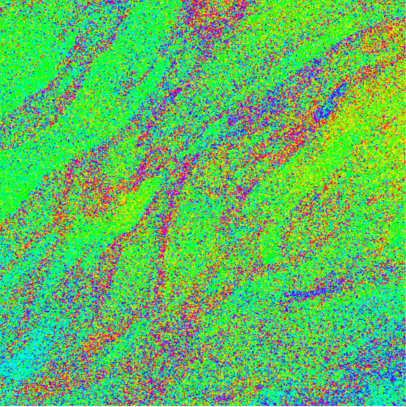
\includegraphics[width=.20\linewidth]{InSAR_ArgVol}}
	\\
	\hspace{0.01cm}
	\subfloat[\centering\label{img_LeeRefined_ArgVol}]{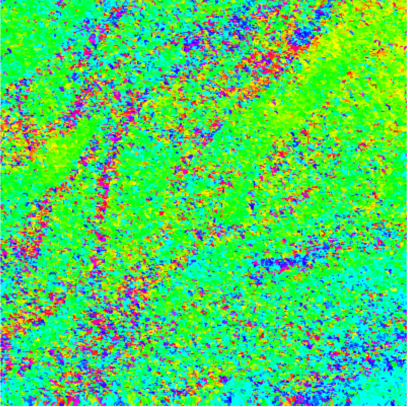
\includegraphics[width=.20\linewidth]{img_LeeRefined_ArgVol}}
	\hspace{0.01cm}
	\subfloat[\centering\label{img_LInSARRFE_ArgVol}]{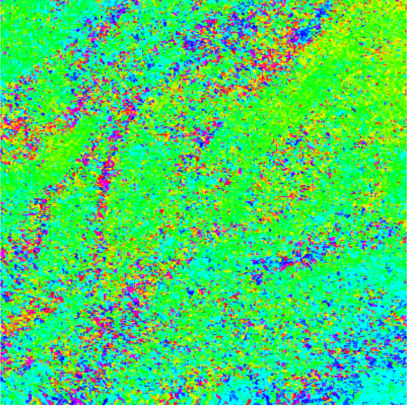
\includegraphics[width=.20\linewidth]{img_LInSARRFE_ArgVol}}
	\hspace{0.01cm}
	\subfloat[\centering\label{img_TcNfilter_ArgVol}]{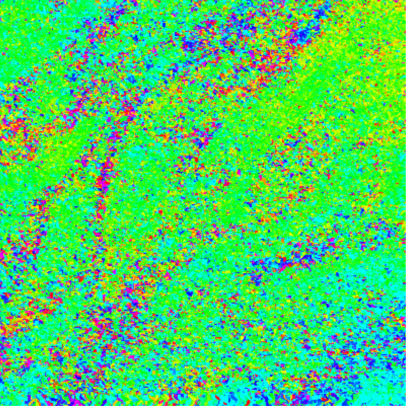
\includegraphics[width=.20\linewidth]{img_TcNfilter_ArgVol}}
	\hspace{0.01cm}
	\subfloat[\centering\label{img_TcCfilter_ArgVol}]{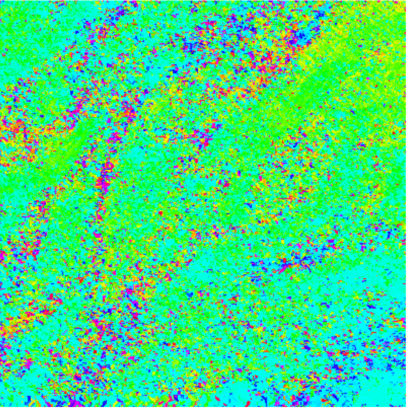
\includegraphics[width=.20\linewidth]{img_TcCfilter_ArgVol}}
	\\
	{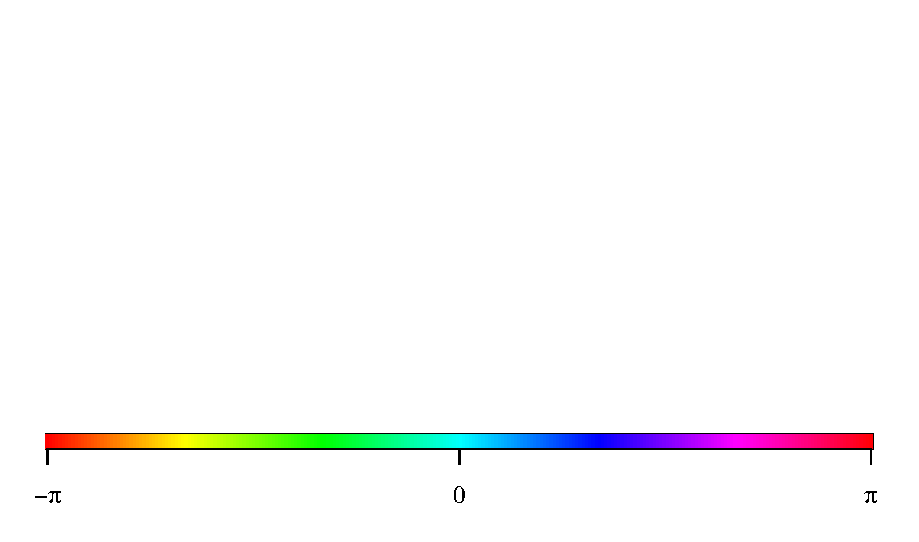
\includegraphics[width=.67\linewidth]{BarraCores}}
	\\	
	\hspace{0.01cm}
	\subfloat[\centering\label{unwrap_LeeRefined_ArgVol}]{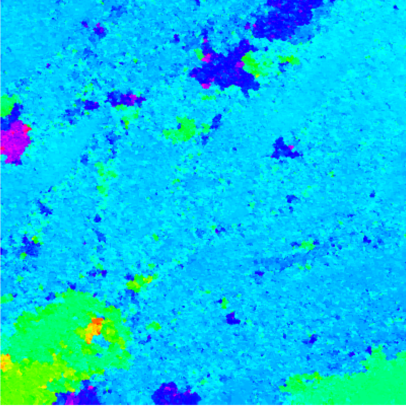
\includegraphics[width=.20\linewidth]{unwrap_LeeRefined_ArgVol}}
	\hspace{0.01cm}
	\subfloat[\centering\label{unwrap_LInSARRFE_ArgVol}]{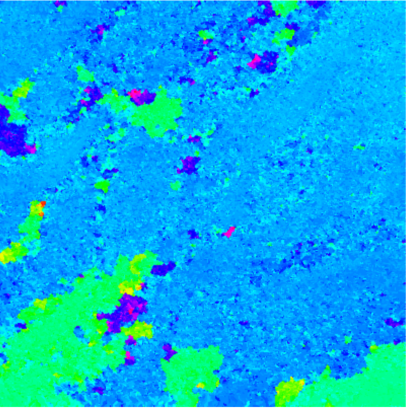
\includegraphics[width=.20\linewidth]{unwrap_LInSARRFE_ArgVol}}
	\hspace{0.01cm}
	\subfloat[\centering\label{unwrap_TcNfilter_ArgVol}]{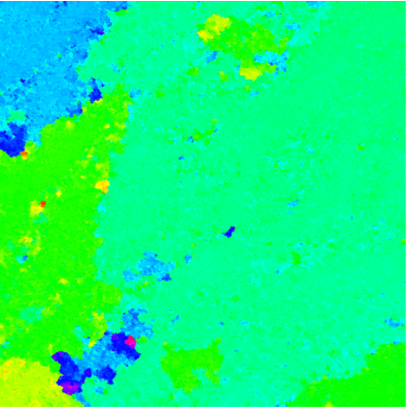
\includegraphics[width=.20\linewidth]{unwrap_TcNfilter_ArgVol}}
	\hspace{0.01cm} 
	\subfloat[\centering\label{unwrap_TcCfilter_ArgVol}]{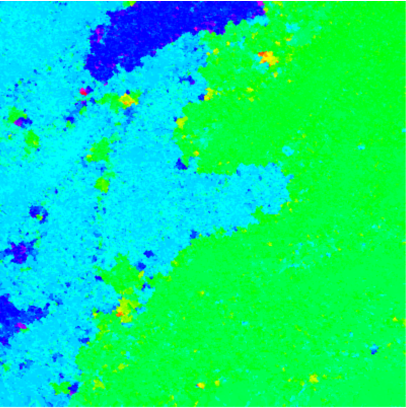
\includegraphics[width=.20\linewidth]{unwrap_TcCfilter_ArgVol}}
	\\
	\vspace{-0.3cm}
	\subfloat{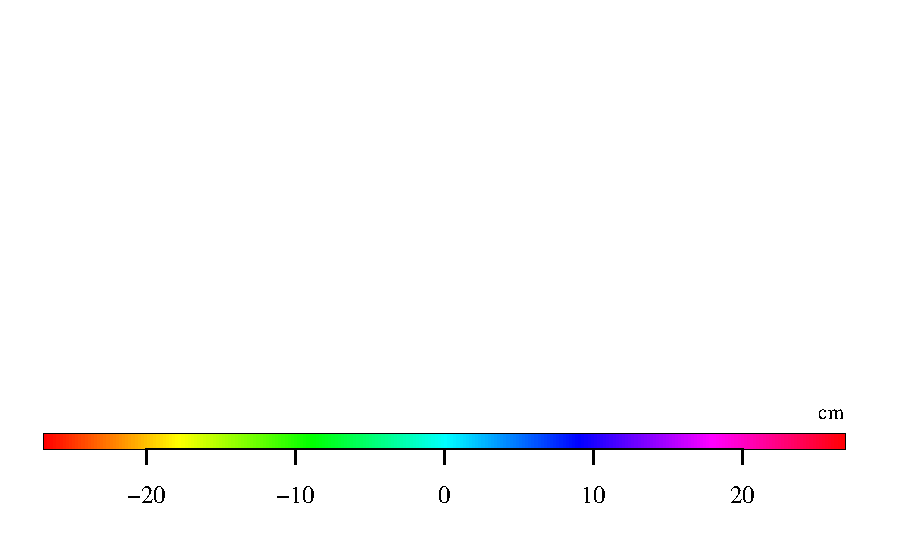
\includegraphics[width=.67\linewidth]{BarraCores_unwrap1}}
	%\end{adjustwidth}
	%\caption{\textmd{Interferograms filtered and before unwrapping the phase (top) and after unwrapping (bottom)}}
	\caption{Robledo Volcano image before and after filtering: (\textbf{a})~Unfiltered Phase, (\textbf{b})~Refined Lee, (\textbf{c})~LInSARRFE, (\textbf{d})~TcNfilter, (\textbf{e})~TcCfilter. Unwrapped phase after filter application: (\textbf{f})~Refined Lee, (\textbf{g})~LInSARRFE, (\textbf{h})~TcNfilter, (\textbf{i})~TcCfilter}
	\label{filters_ArgVol} % label da figura toda
\end{figure}

Tests conducted on images from Los Alamos and the Robledo Volcano revealed consistent behavior. 
Regarding noise reduction, the TcCfilter achieved the best performance, reducing residual noise by \qty{65}{\percent} for the Los Alamos image and \qty{66}{\percent} for the Robledo Volcano image. 
In terms of computational efficiency, the TcNfilter delivered the fastest runtime on the Los Alamos image, saving \qty{77}{\percent} of the time. 
In contrast, for the Robledo Volcano image, the TcNfilter provided the best runtime, saving \qty{79}{\percent} of the time. 

The results also indicate that noise reduction was more effective in images acquired with the Sentinel‑1 sensor than in those acquired with the UAVSAR sensor. 
A similar pattern was observed in computational efficiency, which was higher for the Sentinel‑1 image than for the UAVSAR images. 
Nevertheless, further studies are required to conclusively determine whether the filters applied to Sentinel‑1 imagery are indeed superior to those used with UAVSAR data.

\subsection{Computational performance of the proposed filters compared to the Refined Lee filter}\label{run_time}

Figure~\ref{tempo_otmizado} compares the computational efficiency of the proposed filters (LInSARRFE, TcNfilter, and TcCfilter) with the Refined Lee filter. 
The plot shows evaluations of the proposed filters on simulated and SAR data (La Cumbre Volcano, Los Alamos, Robledo Volcano).

\begin{figure}[hbt]
	{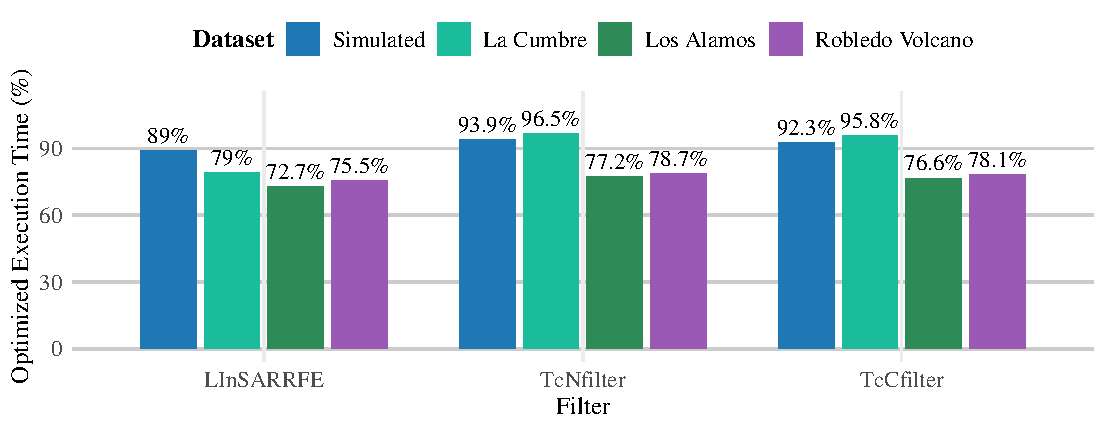
\includegraphics[width=0.9\textwidth]{runtime}}
	\caption{\textmd{Optimized Execution Time}}
	\label{tempo_otmizado}
\end{figure}

The impacts of the proposed filters are highly positive, demonstrating both effectiveness and efficiency in terms of processing time. 
The plot shows that the proposed filters significantly outperform the Refined Lee filter in terms of computational efficiency. 
These results indicate that LInSARRFE, TcNfilter, and TcCfilter are practical and robust options for noise reduction in InSAR data, particularly in scenarios where large datasets must be processed within time constraints.
%
%############################ Aqui
%
%%%%%%%%%%%%%%%%%%%%%%%%%%%%%%%%%%%%%%%%%%
\section{Discussion}\label{Discussion}

In this section, we present the main results of applying the proposed filters to simulated and SAR interferometric data. 
We interpret these results in the context of previous studies. 
We also explore the methodological contributions, limitations, and future research directions, considering the challenges of processing large volumes of interferometric data.

\subsection{Performance of the Proposed Filters}

The LInSARRFE, TcNfilter, and TcCfilter filters effectively reduce phase noise. 
TcNfilter achieved the bigest RT values in simulated data, indicating high save time in phase estimation, without compromising accuracy. 
The LInSARRFE and TcNfilter filters also preserved image structures, maintaining SSIM values similar to those of the Refined Lee filter. 
This balance between smoothing and detail preservation is crucial for preserving the information in interferograms.

\subsection{Methodological Contributions}

The proposed framework uses circular physical statistical models and truncated empirical distributions to adaptively select filtering windows that reflect local phase variability. Unlike traditional approaches that use fixed window sizes or intensity-based criteria, the proposed filters use a probabilistic formulation that improves robustness in heterogeneous interferometric regions.

The authors highlight that, in this work, we investigated the change from the Lee model to the Gierull physical model and to empirical models, a methodology that demonstrated improvements in computational efficiency.


The Refined Lee InSAR filter was chosen as the benchmark because it’s the widely employed spatial-domain statistical filtering method from which both the Enhanced Refined Lee variant and the methods in this work are derived. A broader comparison of all Lee filter variants is beyond the scope of this study and warrants future investigation.


Using Gierull's formulation for the phase distribution~\eqref{subsec:sec3.2.1_cap3Eq8} leads to a favorable tradeoff between residual suppression and computational efficiency. 
An additional advantage of this physically based formulation is its ability to extract coherence information directly from the noisy interferogram. 
%As illustrated in Fig.~\ref{fig:coherence_insar}, the coherence map obtained for the Los Alamos interferogram—shown on the right—demonstrates the potential of this approach for subsequent analysis in future applications.

\subsection{Computational Efficiency}
Computational efficiency was crucial in the evaluation of the proposed filters.
The TcNfilter and TcCfilter showed significantly shorter run times than the Refined Lee filter, proving that noise reduction can be achieved at lower computational cost. 
The LInSARRFE filter combined acceptable computational performance with high accuracy, making it a competitive alternative for processing large volumes of interferometric data. 
These characteristics are promising given the growing demand for efficient algorithms in missions such as NISAR, which generate massive amounts of interferometric data.

\subsection{Study limitations}

The evaluation of the filters was based on a limited number of scenarios, which may limit generalisation. 
Adjusting filtering parameters, especially the coherence map, is not yet automated, which may limit broader use. 
The methods assume local phase homogeneity, which may not hold in areas with strong decorrelation or complex topography. 
Another challenge is the numerical integration required during filtering, which affects performance. Further research is needed to improve integration techniques, including parallel computing.

\subsection{Perspectives for Future Work}

Considering the findings of this research, several perspectives for future investigations emerge. One suggested area of focus is the further analysis of the convergence of physical models for phase difference. For example, for non-integer real values of $L$, the model defined in~\eqref{subsec:sec3.2.1_cap3Eq7} works. 
On the other hand, the expression presented in~\eqref{subsec:sec3.2.1_cap3Eq8}, obviously, does not. 
However, a linear or quadratic interpolation of the phase values between two or more adjacent integer values may also work very well. 
This idea can improve numerical integration.

%Future studies should investigate the underlying reasons why the proposed methods exhibit superior performance in residual reduction when applied to Sentinel-1 InSAR imagery compared to UAVSAR data.

Exploring and developing new empirical models adaptable to different InSAR scenarios represents an interesting approach. 
The integration of machine learning techniques is a relevant direction, aiming to develop models that learn specific patterns in SAR images and automatically adjust filter parameters, thereby representing a significant advance in the effectiveness of these approaches.

\section{Conclusions}\label{sec:conclusions}

This study introduced and evaluated three filtering approaches, LInSARRFE, TcNfilter, and TcCfilter, to reduce phase noise in InSAR interferograms with low computational cost. 
Their performance was assessed using simulated and SAR interferometric images from the Sentinel-1 (C-band) and UAVSAR (L-band) sensors. 
We used as a baseline the Refined Lee InSAR filter, and assessed accuracy, structural preservation, and computational efficiency.

The simulated dataset, a noise-free reference, enabled quantitative evaluation using RMSE, SSIM, and runtime. 
TcCfilter showed the lowest RMSE, indicating superior accuracy. 
All proposed methods maintained SSIM values comparable to the Refined Lee filter, suppressing noise without compromising structural information. 
In terms of computational efficiency, the proposed filters were notably faster, with TcNfilter achieving a nearly \qty{92}{\percent} reduction in runtime compared to the Refined Lee filter, making it suitable for large-scale InSAR applications.

In the real SAR datasets (La Cumbre, Los Alamos, and Robledo Volcano), filter quality was assessed using phase residuals and runtime. 
All proposed methods reduced residuals as much as or more than the Refined Lee filter. 
The TcCfilter had the best noise reduction, while the TcNfilter had the fastest processing times, reducing over \qty{96}{\percent} in some cases. 
These results show that the proposed filters balance smoothing and detail preservation, which is crucial for reliable phase unwrapping.

Testing with Sentinel-1 data showed greater reductions in phase residuals and better computational performance than UAVSAR data when processed with the proposed methods. The above suggests that the characteristics of Sentinel-1 data better align with the assumptions of the proposed physics-statistical and empirical models. However, further investigation is needed.
%Sentinel-1 data showed systematically greater reductions in phase residuals and better computational performance than UAVSAR data when processed with the proposed methods. 
%This suggests that the characteristics of Sentinel-1 data better match the assumptions of the proposed statistical and empirical models. 
However, further investigation is needed.

Methodologically, this research contributes by integrating circular physical models and truncated empirical models, allowing for adaptive window selection based on local phase variability. 
%The use of the Gierull distribution proved advantageous, offering a favorable balance between filtering performance and computation time, and it allowed the extraction of coherence maps for subsequent analyses. 
These advances present promising directions for improving the processing of future large-scale InSAR missions, such as NISAR, which will generate massive volumes of interferometric data.

%Nevertheless, we highlight some limitations of the methodology. 
%The evaluation covered a limited number of scenarios, and parameter estimation, especially coherence, remains non-automated, which may restrict wider operational applicability. 
%The numerical integration required by filters based on physical principles continues to present significant computational challenges, indicating the need for optimized solvers or parallel processing strategies. 
%Furthermore, the methods assume local phase homogeneity, which may not hold in areas with strong decorrelation or complex topography.

%Future work should investigate:
%\begin{itemize}
%\item Why the proposed filters perform better on Sentinel-1 than on UAVSAR, exploring sensor characteristics, noise models, resolution differences, and coherence distributions.
%
%\item Improved numerical integration methods, including parallelization and interpolation strategies among multilook values.
%
%\item The creation of new empirical models adaptable to diverse interferometric contexts.
%
%\item The integration of machine learning to automate parameter estimation and adapt the filtering process to local image properties.
%\end{itemize}

Overall, the study shows that LInSARRFE, TcNfilter, and TcCfilter are robust, computationally efficient, and high-performance alternatives to traditional InSAR filters. 
Their ability to reduce noise while preserving structural information, combined with significantly reduced computational cost, makes them promising tools for large-scale interferometric applications, both current and emerging.

%%%%%%%%%%%%%%%%%%%%%%%%%%%%%%%%%%%%%%%%%%
\vspace{6pt} 

%%%%%%%%%%%%%%%%%%%%%%%%%%%%%%%%%%%%%%%%%%
%% optional
%\supplementary{The following supporting information can be downloaded at:  \linksupplementary{s1}, Figure S1: title; Table S1: title; Video S1: title.}

% Only for journal Methods and Protocols:
% If you wish to submit a video article, please do so with any other supplementary material.
% \supplementary{The following supporting information can be downloaded at: \linksupplementary{s1}, Figure S1: title; Table S1: title; Video S1: title. A supporting video article is available at doi: link.}

% Only used for preprtints:
% \supplementary{The following supporting information can be downloaded at the website of this paper posted on \href{https://www.preprints.org/}{Preprints.org}.}

% Only for journal Hardware:
% If you wish to submit a video article, please do so with any other supplementary material.
% \supplementary{The following supporting information can be downloaded at: \linksupplementary{s1}, Figure S1: title; Table S1: title; Video S1: title.\vspace{6pt}\\
%\begin{tabularx}{\textwidth}{lll}
%\toprule
%\textbf{Name} & \textbf{Type} & \textbf{Description} \\
%\midrule
%S1 & Python script (.py) & Script of python source code used in XX \\
%S2 & Text (.txt) & Script of modelling code used to make Figure X \\
%S3 & Text (.txt) & Raw data from experiment X \\
%S4 & Video (.mp4) & Video demonstrating the hardware in use \\
%... & ... & ... \\
%\bottomrule
%\end{tabularx}
%}

%%%%%%%%%%%%%%%%%%%%%%%%%%%%%%%%%%%%%%%%%%
\authorcontributions{The authors attest to having contributed equally to this research. All phases of the work, ranging from the development of the methodology to the preparation and revision of the manuscript, were conducted collaboratively.}


\funding{
Professor Anderson Adaime de Borba declares that this work was partly funded by the Mackenzie Research and Innovation Fund  ``Mackpesquisa,'' under grant project nº~261029 MACK - 0018156.}

%\institutionalreview{In this section, you should add the Institutional Review Board Statement and approval number, if relevant to your study. You might choose to exclude this statement if the study did not require ethical approval. Please note that the Editorial Office might ask you for further information. Please add “The study was conducted in accordance with the Declaration of Helsinki, and approved by the Institutional Review Board (or Ethics Committee) of NAME OF INSTITUTE (protocol code XXX and date of approval).” for studies involving humans. OR “The animal study protocol was approved by the Institutional Review Board (or Ethics Committee) of NAME OF INSTITUTE (protocol code XXX and date of approval).” for studies involving animals. OR “Ethical review and approval were waived for this study due to REASON (please provide a detailed justification).” OR “Not applicable” for studies not involving humans or animals.}

%\informedconsent{Any research article describing a study involving humans should contain this statement. Please add ``Informed consent was obtained from all subjects involved in the study.'' OR ``Patient consent was waived due to REASON (please provide a detailed justification).'' OR ``Not applicable'' for studies not involving humans. You might also choose to exclude this statement if the study did not involve humans.

%Written informed consent for publication must be obtained from participating patients who can be identified (including by the patients themselves). Please state ``Written informed consent has been obtained from the patient(s) to publish this paper'' if applicable.}

\dataavailability{The code and data supporting this study are publicly available at~\url{https://github.com/araujoUFPE}. And, the UAVSAR data was obtained from~\url{http://uavsar.jpl.nasa.gov/}
} 

% Only for journal Drones
%\durcstatement{Current research is limited to the [please insert a specific academic field, e.g., XXX], which is beneficial [share benefits and/or primary use] and does not pose a threat to public health or national security. Authors acknowledge the dual-use potential of the research involving xxx and confirm that all necessary precautions have been taken to prevent potential misuse. As an ethical responsibility, authors strictly adhere to relevant national and international laws about DURC. Authors advocate for responsible deployment, ethical considerations, regulatory compliance, and transparent reporting to mitigate misuse risks and foster beneficial outcomes.}

% Only for journal Nursing Reports
%\publicinvolvement{Please describe how the public (patients, consumers, carers) were involved in the research. Consider reporting against the GRIPP2 (Guidance for Reporting Involvement of Patients and the Public) checklist. If the public were not involved in any aspect of the research add: ``No public involvement in any aspect of this research''.}
%
%% Only for journal Nursing Reports
%\guidelinesstandards{Please add a statement indicating which reporting guideline was used when drafting the report. For example, ``This manuscript was drafted against the XXX (the full name of reporting guidelines and citation) for XXX (type of research) research''. A complete list of reporting guidelines can be accessed via the equator network: \url{https://www.equator-network.org/}.}
%
%% Only for journal Nursing Reports
%\useofartificialintelligence{Please describe in detail any and all uses of artificial intelligence (AI) or AI-assisted tools used in the preparation of the manuscript. This may include, but is not limited to, language translation, language editing and grammar, or generating text. Alternatively, please state that “AI or AI-assisted tools were not used in drafting any aspect of this manuscript”.}

%\acknowledgments{In this section you can acknowledge any support given which is not covered by the author contribution or funding sections. This may include administrative and technical support, or donations in kind (e.g., materials used for experiments). Where GenAI has been used for purposes such as generating text, data, or graphics, or for study design, data collection, analysis, or interpretation of data, please add “During the preparation of this manuscript/study, the author(s) used [tool name, version information] for the purposes of [description of use]. The authors have reviewed and edited the output and take full responsibility for the content of this publication.”}

\conflictsofinterest{The authors declare no conflicts of interest.} 

%%%%%%%%%%%%%%%%%%%%%%%%%%%%%%%%%%%%%%%%%%
%% Optional

%% Only for journal Encyclopedia
%\entrylink{The Link to this entry published on the encyclopedia platform.}

%\abbreviations{Abbreviations}{
%The following abbreviations are used in this manuscript:
%\\

%\noindent 
%\begin{tabular}{@{}ll}
%MDPI & Multidisciplinary Digital Publishing Institute\\
%DOAJ & Directory of open access journals\\
%TLA & Three letter acronym\\
%LD & Linear dichroism
%\end{tabular}
%}

%%%%%%%%%%%%%%%%%%%%%%%%%%%%%%%%%%%%%%%%%%
%% Optional
%\appendixtitles{no} % Leave argument "no" if all appendix headings stay EMPTY (then no dot is printed after "Appendix A"). If the appendix sections contain a heading then change the argument to "yes".
%\appendixstart
%\appendix
%\section[\appendixname~\thesection]{}
%\subsection[\appendixname~\thesubsection]{}
%The appendix is an optional section that can contain details and data supplemental to the main text---for example, explanations of experimental details that would disrupt the flow of the main text but nonetheless remain crucial to understanding and reproducing the research shown; figures of replicates for experiments of which representative data are shown in the main text can be added here if brief, or as Supplementary Data. Mathematical proofs of results not central to the paper can be added as an appendix.

%\begin{table}[hbt] 
%\caption{This is a table caption.\label{tab5}}
%\newcolumntype{C}{>{\centering\arraybackslash}X}
%\begin{tabularx}{\textwidth}{CCC}
%\toprule
%\textbf{Title 1}	& \textbf{Title 2}	& \textbf{Title 3}\\
%\midrule
%Entry 1		& Data			& Data\\
%Entry 2		& Data			& Data\\
%\bottomrule
%\end{tabularx}
%\end{table}

%\section[\appendixname~\thesection]{}
%All appendix sections must be cited in the main text. In the appendices, Figures, Tables, etc. should be labeled, starting with ``A''---e.g., Figure A1, Figure A2, etc.

%%%%%%%%%%%%%%%%%%%%%%%%%%%%%%%%%%%%%%%%%%
\isPreprints{}{% This command is only used for ``preprints''.
\begin{adjustwidth}{-\extralength}{0cm}
} % If the paper is ``preprints'', please uncomment this parenthesis.
\printendnotes[custom] % Un-comment to print a list of endnotes

\reftitle{References}

\bibliography{bibliografia1}
\PublishersNote{}
%\isPreprints{}{% This command is only used for ``preprints''.
\end{adjustwidth}
%} % If the paper is ``preprints'', please uncomment this parenthesis.
\end{document}

